% Options for packages loaded elsewhere
\PassOptionsToPackage{unicode}{hyperref}
\PassOptionsToPackage{hyphens}{url}
\PassOptionsToPackage{dvipsnames,svgnames,x11names}{xcolor}
%
\documentclass[
  12pt,
]{krantz}
\usepackage{amsmath,amssymb}
\usepackage{iftex}
\ifPDFTeX
  \usepackage[T1]{fontenc}
  \usepackage[utf8]{inputenc}
  \usepackage{textcomp} % provide euro and other symbols
\else % if luatex or xetex
  \usepackage{unicode-math} % this also loads fontspec
  \defaultfontfeatures{Scale=MatchLowercase}
  \defaultfontfeatures[\rmfamily]{Ligatures=TeX,Scale=1}
\fi
\usepackage{lmodern}
\ifPDFTeX\else
  % xetex/luatex font selection
\fi
% Use upquote if available, for straight quotes in verbatim environments
\IfFileExists{upquote.sty}{\usepackage{upquote}}{}
\IfFileExists{microtype.sty}{% use microtype if available
  \usepackage[]{microtype}
  \UseMicrotypeSet[protrusion]{basicmath} % disable protrusion for tt fonts
}{}
\usepackage{xcolor}
\usepackage{color}
\usepackage{fancyvrb}
\newcommand{\VerbBar}{|}
\newcommand{\VERB}{\Verb[commandchars=\\\{\}]}
\DefineVerbatimEnvironment{Highlighting}{Verbatim}{commandchars=\\\{\}}
% Add ',fontsize=\small' for more characters per line
\usepackage{framed}
\definecolor{shadecolor}{RGB}{248,248,248}
\newenvironment{Shaded}{\begin{snugshade}}{\end{snugshade}}
\newcommand{\AlertTok}[1]{\textcolor[rgb]{0.94,0.16,0.16}{#1}}
\newcommand{\AnnotationTok}[1]{\textcolor[rgb]{0.56,0.35,0.01}{\textbf{\textit{#1}}}}
\newcommand{\AttributeTok}[1]{\textcolor[rgb]{0.13,0.29,0.53}{#1}}
\newcommand{\BaseNTok}[1]{\textcolor[rgb]{0.00,0.00,0.81}{#1}}
\newcommand{\BuiltInTok}[1]{#1}
\newcommand{\CharTok}[1]{\textcolor[rgb]{0.31,0.60,0.02}{#1}}
\newcommand{\CommentTok}[1]{\textcolor[rgb]{0.56,0.35,0.01}{\textit{#1}}}
\newcommand{\CommentVarTok}[1]{\textcolor[rgb]{0.56,0.35,0.01}{\textbf{\textit{#1}}}}
\newcommand{\ConstantTok}[1]{\textcolor[rgb]{0.56,0.35,0.01}{#1}}
\newcommand{\ControlFlowTok}[1]{\textcolor[rgb]{0.13,0.29,0.53}{\textbf{#1}}}
\newcommand{\DataTypeTok}[1]{\textcolor[rgb]{0.13,0.29,0.53}{#1}}
\newcommand{\DecValTok}[1]{\textcolor[rgb]{0.00,0.00,0.81}{#1}}
\newcommand{\DocumentationTok}[1]{\textcolor[rgb]{0.56,0.35,0.01}{\textbf{\textit{#1}}}}
\newcommand{\ErrorTok}[1]{\textcolor[rgb]{0.64,0.00,0.00}{\textbf{#1}}}
\newcommand{\ExtensionTok}[1]{#1}
\newcommand{\FloatTok}[1]{\textcolor[rgb]{0.00,0.00,0.81}{#1}}
\newcommand{\FunctionTok}[1]{\textcolor[rgb]{0.13,0.29,0.53}{\textbf{#1}}}
\newcommand{\ImportTok}[1]{#1}
\newcommand{\InformationTok}[1]{\textcolor[rgb]{0.56,0.35,0.01}{\textbf{\textit{#1}}}}
\newcommand{\KeywordTok}[1]{\textcolor[rgb]{0.13,0.29,0.53}{\textbf{#1}}}
\newcommand{\NormalTok}[1]{#1}
\newcommand{\OperatorTok}[1]{\textcolor[rgb]{0.81,0.36,0.00}{\textbf{#1}}}
\newcommand{\OtherTok}[1]{\textcolor[rgb]{0.56,0.35,0.01}{#1}}
\newcommand{\PreprocessorTok}[1]{\textcolor[rgb]{0.56,0.35,0.01}{\textit{#1}}}
\newcommand{\RegionMarkerTok}[1]{#1}
\newcommand{\SpecialCharTok}[1]{\textcolor[rgb]{0.81,0.36,0.00}{\textbf{#1}}}
\newcommand{\SpecialStringTok}[1]{\textcolor[rgb]{0.31,0.60,0.02}{#1}}
\newcommand{\StringTok}[1]{\textcolor[rgb]{0.31,0.60,0.02}{#1}}
\newcommand{\VariableTok}[1]{\textcolor[rgb]{0.00,0.00,0.00}{#1}}
\newcommand{\VerbatimStringTok}[1]{\textcolor[rgb]{0.31,0.60,0.02}{#1}}
\newcommand{\WarningTok}[1]{\textcolor[rgb]{0.56,0.35,0.01}{\textbf{\textit{#1}}}}
\usepackage{longtable,booktabs,array}
\usepackage{calc} % for calculating minipage widths
% Correct order of tables after \paragraph or \subparagraph
\usepackage{etoolbox}
\makeatletter
\patchcmd\longtable{\par}{\if@noskipsec\mbox{}\fi\par}{}{}
\makeatother
% Allow footnotes in longtable head/foot
\IfFileExists{footnotehyper.sty}{\usepackage{footnotehyper}}{\usepackage{footnote}}
\makesavenoteenv{longtable}
\usepackage{graphicx}
\makeatletter
\def\maxwidth{\ifdim\Gin@nat@width>\linewidth\linewidth\else\Gin@nat@width\fi}
\def\maxheight{\ifdim\Gin@nat@height>\textheight\textheight\else\Gin@nat@height\fi}
\makeatother
% Scale images if necessary, so that they will not overflow the page
% margins by default, and it is still possible to overwrite the defaults
% using explicit options in \includegraphics[width, height, ...]{}
\setkeys{Gin}{width=\maxwidth,height=\maxheight,keepaspectratio}
% Set default figure placement to htbp
\makeatletter
\def\fps@figure{htbp}
\makeatother
\setlength{\emergencystretch}{3em} % prevent overfull lines
\providecommand{\tightlist}{%
  \setlength{\itemsep}{0pt}\setlength{\parskip}{0pt}}
\setcounter{secnumdepth}{5}
\usepackage{ctex} % used to render chinese in pdf
\setCJKmainfont{KaiTi}
\usepackage{indentfirst} % used to add indent to first block of each section
\usepackage{booktabs}
\usepackage{longtable}
\usepackage[bf,singlelinecheck=off]{caption}

\usepackage{Alegreya}
\usepackage[scale=.7]{sourcecodepro}

\usepackage{framed,color}
\definecolor{shadecolor}{RGB}{248,248,248}

\renewcommand{\textfraction}{0.05}
\renewcommand{\topfraction}{0.8}
\renewcommand{\bottomfraction}{0.8}
\renewcommand{\floatpagefraction}{0.75}

\renewenvironment{quote}{\begin{VF}}{\end{VF}}
\usepackage{hyperref}
\let\oldhref\href
\renewcommand{\href}[2]{#2\footnote{\url{#1}}}

\ifxetex
  \usepackage{letltxmacro}
  \setlength{\XeTeXLinkMargin}{1pt}
  \LetLtxMacro\SavedIncludeGraphics\includegraphics
  \def\includegraphics#1#{% #1 catches optional stuff (star/opt. arg.)
    \IncludeGraphicsAux{#1}%
  }%
  \newcommand*{\IncludeGraphicsAux}[2]{%
    \XeTeXLinkBox{%
      \SavedIncludeGraphics#1{#2}%
    }%
  }%
\fi

\makeatletter
\newenvironment{kframe}{%
\medskip{}
\setlength{\fboxsep}{.8em}
 \def\at@end@of@kframe{}%
 \ifinner\ifhmode%
  \def\at@end@of@kframe{\end{minipage}}%
  \begin{minipage}{\columnwidth}%
 \fi\fi%
 \def\FrameCommand##1{\hskip\@totalleftmargin \hskip-\fboxsep
 \colorbox{shadecolor}{##1}\hskip-\fboxsep
     % There is no \\@totalrightmargin, so:
     \hskip-\linewidth \hskip-\@totalleftmargin \hskip\columnwidth}%
 \MakeFramed {\advance\hsize-\width
   \@totalleftmargin\z@ \linewidth\hsize
   \@setminipage}}%
 {\par\unskip\endMakeFramed%
 \at@end@of@kframe}
\makeatother

\makeatletter
\@ifundefined{Shaded}{
}{\renewenvironment{Shaded}{\begin{kframe}}{\end{kframe}}}
\makeatother

\newenvironment{rmdblock}[1]
  {
  \begin{itemize}
  \renewcommand{\labelitemi}{
    \raisebox{-.7\height}[0pt][0pt]{
      {\setkeys{Gin}{width=3em,keepaspectratio}\includegraphics{images/#1}}
    }
  }
  \setlength{\fboxsep}{1em}
  \begin{kframe}
  \item
  }
  {
  \end{kframe}
  \end{itemize}
  }
\newenvironment{rmdnote}
  {\begin{rmdblock}{note}}
  {\end{rmdblock}}
\newenvironment{rmdcaution}
  {\begin{rmdblock}{caution}}
  {\end{rmdblock}}
\newenvironment{rmdimportant}
  {\begin{rmdblock}{important}}
  {\end{rmdblock}}
\newenvironment{rmdtip}
  {\begin{rmdblock}{tip}}
  {\end{rmdblock}}
\newenvironment{rmdwarning}
  {\begin{rmdblock}{warning}}
  {\end{rmdblock}}

\usepackage{makeidx}
\makeindex

\urlstyle{tt}

\usepackage{amsthm}
\makeatletter
\def\thm@space@setup{%
  \thm@preskip=8pt plus 2pt minus 4pt
  \thm@postskip=\thm@preskip
}
\makeatother

\frontmatter
\ifLuaTeX
  \usepackage{selnolig}  % disable illegal ligatures
\fi
\usepackage[]{natbib}
\bibliographystyle{apalike}
\usepackage{bookmark}
\IfFileExists{xurl.sty}{\usepackage{xurl}}{} % add URL line breaks if available
\urlstyle{same}
\hypersetup{
  pdftitle={Bookdown: 使用 R Markdown 创作书籍和技术文档},
  pdfauthor={Yihui Xie},
  colorlinks=true,
  linkcolor={Maroon},
  filecolor={Maroon},
  citecolor={Blue},
  urlcolor={Blue},
  pdfcreator={LaTeX via pandoc}}

\title{Bookdown: 使用 R Markdown 创作书籍和技术文档}
\author{Yihui Xie}
\date{2024-11-04}

\usepackage{amsthm}
\newtheorem{theorem}{定理}[chapter]
\newtheorem{lemma}{引理}[chapter]
\newtheorem{corollary}{推论}[chapter]
\newtheorem{proposition}{命题}[chapter]
\newtheorem{conjecture}{猜想}[chapter]
\theoremstyle{definition}
\newtheorem{definition}{定义}[chapter]
\theoremstyle{definition}
\newtheorem{example}{例}[chapter]
\theoremstyle{definition}
\newtheorem{exercise}{练习}[chapter]
\theoremstyle{definition}
\newtheorem{hypothesis}{假设}[chapter]
\theoremstyle{remark}
\newtheorem*{remark}{Remark}
\newtheorem*{solution}{解}
\begin{document}
\maketitle

%\cleardoublepage\newpage\thispagestyle{empty}\null
%\cleardoublepage\newpage\thispagestyle{empty}\null
%\cleardoublepage\newpage
\thispagestyle{empty}
\begin{center}
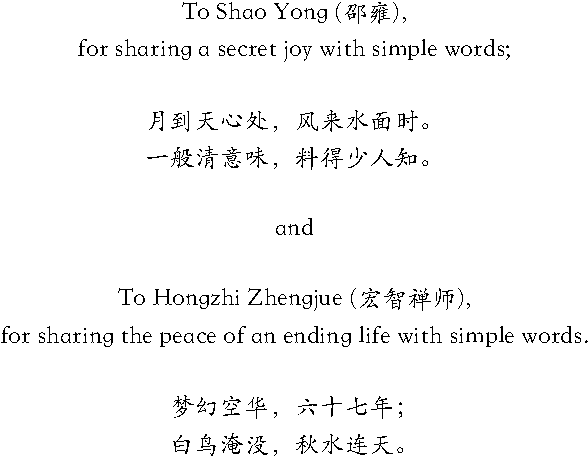
\includegraphics{images/dedication.pdf}
\end{center}

\setlength{\abovedisplayskip}{-5pt}
\setlength{\abovedisplayshortskip}{-5pt}

{
\hypersetup{linkcolor=}
\setcounter{tocdepth}{2}
\tableofcontents
}
\listoffigures
\listoftables
\chapter*{翻译与排版说明}\label{ux7ffbux8bd1ux4e0eux6392ux7248ux8bf4ux660e}


原书为 \href{https://bookdown.org/yihui/bookdown/}{\emph{bookdown: Authoring Books and Technical Documents with R Markdown}}。

原书简体中文版还没有影子,所以笔者先用自己早就遗忘的文学素养进行翻译,使用与原书相同的技术栈生成简体中文版的书籍。

\section*{翻译说明}\label{ux7ffbux8bd1ux8bf4ux660e}


将英文技术书籍翻译为中文是个痛苦的过程,难以避免地会遇到一些没有公认翻译方式的英文词汇,或者是有公认的中文翻译词汇,但该词过于口语化,或者不能很好地反映英文词汇的意思。这些英文词汇以及它们在书中的对应中文词汇将在下方列出,欢迎大家批评。

\begin{longtable}[]{@{}
  >{\raggedright\arraybackslash}p{(\columnwidth - 4\tabcolsep) * \real{0.2000}}
  >{\raggedright\arraybackslash}p{(\columnwidth - 4\tabcolsep) * \real{0.4000}}
  >{\raggedright\arraybackslash}p{(\columnwidth - 4\tabcolsep) * \real{0.4000}}@{}}
\toprule\noalign{}
\begin{minipage}[b]{\linewidth}\raggedright
英文词汇
\end{minipage} & \begin{minipage}[b]{\linewidth}\raggedright
中文翻译
\end{minipage} & \begin{minipage}[b]{\linewidth}\raggedright
原因
\end{minipage} \\
\midrule\noalign{}
\endhead
\bottomrule\noalign{}
\endlastfoot
package & 软件包,程序包 & r pkgs 是一组用来完成特定任务的程序,作为 R 的补充,符合 Software Package 的定义。 \\
hardcopy & 实体书,书的实体版本 & 原意为``硬拷贝'',指信息被储存并显示在物体实体上,这里采用符合常用语境的翻译。 \\
page margin & 页边空白 & 直译为页面外边距(区域),是页面各边边线离矩形文字区域的垂直距离,四边共同组成了边框形状的区域,通常为空白部分。 \\
typewriter font & 老式打字机字体 & 直译为``打字机字体'',也就是类似于二十世纪七八十年代的铅字打字机的字体,为突出其独特性而强调了``老式'' \\
R plots & (R 语言输出的图片) & (暂无) \\
personal access token & 个人访问令牌 & 参照国内计网教科书对于 token 的翻译进行的直译。 \\
command-line & 命令行(hang,第二声)、命令提示符 & 笔者对于``line''所指的概念不明确,因此参照国内流行的翻译,称为``命令行''。 \\
key & 字段、配置项 & 指的是 YAML 文件中的配置项,位于冒号 \texttt{:} 左侧。由于是``键值对''的形式,因此用了 key 一词,但依照语境翻译为``字段''或是``配置项''。 \\
LaTeX preamble & LaTeX preamble、LaTeX 导言 & 在 \texttt{\textbackslash{}begin\{document\}} 之前的命令称为 ``preamble''(导言),preamble 中通常定义文档的格式、语言等。 \\
Small Capitals & 小型大写字母 & 西文字体设计中的一种字符形式,其大写字母的字高一般与 `x' 等高,并在笔画上做一定的修正,保持更宽的纵横比以保证可读性。 \\
dedication page & 献词页 & 在一些书中,作者想要把这本书献给某人,献词通常写在前几页。 \\
quote & 引用环境(文段) & LaTeX 中的 Quote 环境,放置引用于其他文献中的文段。 \\
copyeditor & 定稿编辑 & 文稿最后付印时按照印刷出版要求进行排版、校正文字和格式错误的编辑。 \\
typeface & 字型 & typeface 与 font 有着微妙的区别,本书中将前者翻译为``字型'',后者翻译为``字体''。且前者多指代印刷用字体。 \\
help desk & 帮助中心 & 直译为``帮助台'',是用来解决用户的 IT 服务问题,降低处置时间的一个服务。 \\
demo & 样例 & 为与 example 区分,demo 翻译为样例,example 翻译为示例。 \\
final words & 结语 & 翻译为中文书籍中常见的``结语''。 \\
index & 主页 & 当描述对象为网页时,翻译为``主页'',指网站的入口点。 \\
in this case & 使用这种方法时 & 将原意``在这种情况下''翻译得更加具体一些。 \\
render & 编译、呈现为、转化为 & 在图形学中一直被翻译为``渲染'',但用在本书中并不合适。考虑到本书中书籍是由源文档\textbf{转化为}多种格式的书籍,其过程涉及源文档的转译(Markdown to LaTeX)与编码,因此翻译为``编译''。另外,它也有``呈现''的意思,在本书中的一些语境下适用。 \\
knit & 生成、``编织'' & 这个词是对于将代码和文字交织在一起的文学编程的形象描述,笔者暂且找不到一个好的词来准确描述该过程,因此使用``生成''或加了双引号的``编织''一词来翻译。 \\
isolate & 剔除 & 作``分离''、``剔除''解释。 \\
side-effects & 副作用 & 这里指程序设计中的``副作用''。如果一个函数修改了自己范围之外的资源,例如读取文件、调用其它有副作用的函数,则该函数称作是有副作用的。 \\
upgrade/update & 升级/更新 & \\
serve (v.) & 通过 HTTP 服务 & 直译并不贴切,因此用其行为和原理来解释这个词。 \\
daemonized server & 守护进程(?) & 中文互联网上少见``守护服务器''这一词汇,因此将``server''作``服务程序''解,翻译为``守护进程'',日后再行修订。 \\
caret & 脱字符、补注符 & 也就是 \texttt{\^{}},以往文章中漏了字就使用该符号标注插入的字。 \\
blockquote & 块引用 & 拆分为 block 和 quote 两部分翻译,意思为作为块级元素的引用文段。 \\
fenced \texttt{div} syntax & \texttt{div} 围栏语法 & 来源于 Pandoc 的 \texttt{fenced\ div\ block},可以使用至少三个连续的 \texttt{:} 和属性构造原生的 \texttt{Div} 块,由于类似于围栏,因此翻译为``围栏语法''。 \\
token & 令牌、标志 & 当语境中没有``通行证''等类似含义时,使用``标志''翻译。 \\
part title & 各部份的标题? & 意思为将书籍中的部分章节组成一个部分,例如第 1、2、3 章组成第一部分,为这一部分的标题。 \\
aspect ratio & 纵横比 & 专业词汇 \\
logo & 徽标 & 相比于``标志''和``标识''这两种具有广泛含义的词汇,``徽标''这个翻译简洁且准确。 \\
chunk & 区块、代码块 & 泛用含义为``区块'',多用于标识 R 代码。 \\
section ID & 章节标识符 & 为准确表达其实质含义,这里 ID 翻译为``标识符'',意为能够标识一个章节的\textbf{符号}。 \\
item & 项目、文档项目 & 在本文部分语境下,item 指文档中如章节标题、文本、引用等项目。(日后润色) \\
manual & 使用指南 & 翻译时突出``指南''这一功能性的特点,弱化``手册''这一形式上的特点。 \\
citation key & 引文关键词 & CS 中 key 一般直接翻译为``键'',指的是``键-值''类型的数据结构,拥有一一对应的关系,由于本书目标读者并不是 CS 专业人群,因此以更加通俗的``关键词''来体现``索引''的关系。 \\
braces & 圆括号 & 一般被译为``大括号'',此处强调其形状,翻译为``圆括号'',因为通常所说的大括号一般指的是\texttt{\{\}},即花括号。 \\
vignette & 说明短文 & (说明事物特点的)短文,有一种翻译为``小品文'',但实际上 R 的软件包的 vignette 都是说明性质的,很少带有抒情和叙述文段,且并不是散文文体,因此``小品文''的翻译并不准确。 \\
pipeline sequence & 工作流水线 & 较为贴切的直译为``流水线序列'',但在本文中多反映完成任务所需的多个工作组成的序列,且``流水线''本身隐含有``序列''的意义,因此翻译为``工作流水线''。 \\
reproducible & 可重复的 & 这里特指计算结果能够在他人的平台上以相同的条件重复出来,其对立面是(研究)造假。 \\
tooltip & 提示条 & 指鼠标悬停在部分页面元素上时显示的带有文字的提示框。 \\
toolbar & 工具栏 & \\
sidebar & 侧边栏 & \\
main column & 主栏 & 指网页中用于放置主体内容的列空间。 \\
margin column & 侧栏 & 指网页中用于放置导航、注释等内容的列空间,通常较窄。 \\
full-width figures & 全宽图片(暂) & ``full-width'' 含义未明,可以是整个页面的宽度,也有种解释是页面中文字部分的宽度。 \\
sticky header & 悬浮标题、粘性标题 & 指无论如何滚动网页,页面上总是有一个固定的组件,就像粘在页面上。通常可以是导航栏、网页页头等,能够方便导航。 \\
Project Wizard & 项目向导 & 项目引导程序。 \\
Chapter; Section; Subsection & 章;节;小节 & \\
rant & 吐槽 & 直译为咆哮、叫嚷、夸夸其谈,考虑到宾语为 Twitter,这里翻译为贴近口语的``吐槽''。 \\
Literate Programming & 文学化编程 & 指的是一种将程序代码和文本交织在一起进行说明报告的文档风格。 \\
\end{longtable}

\section*{排版说明}\label{ux6392ux7248ux8bf4ux660e}


由于书中不可避免地会同时出现中文和英文,因此原书的排版并不完全适用于中文翻译版。为了在尊重原书的基础上使页面变得美观,约定如下排版要求:

\begin{enumerate}
\def\labelenumi{\arabic{enumi}.}
\tightlist
\item
  英文单词、标点符号和数字各具有 1 个前导空格和 1 个后导空格。例如:``软件包的名称是 bookdown 吗。''。

  \begin{itemize}
  \tightlist
  \item
    英文单词、标点和数字的一侧为标点符号时,该侧无空格。例如:``使用 Leading and Trailing Spaces。''。
  \end{itemize}
\item
  需要展示并链接 URL 时,将其放入尖括号内 \texttt{\textless{}\textgreater{}}。
\item
  小括号内的文本包含中文时,使用中文小括号 \texttt{()};如果全是英文文本,则使用英文小括号 \texttt{()},并各具有 1 个前导和后导空格。
\item
  书中某些操作中带有选项、菜单等名称,在实际操作时不具有中文翻译,此时列出该单词的中文翻译,后跟括号,括号内展示原英文单词。中文翻译便于读者查询相关资料,原英文单词便于按图索骥地进行操作。
\end{enumerate}

\section*{翻译进度}\label{ux7ffbux8bd1ux8fdbux5ea6}


常言道,人生未填之坑十之八九。笔者学业繁忙,只能利用空闲时间翻译本书。因此在这里记录一下翻译进度,欢迎加入本项目提交 Pull Request。

\begin{longtable}[]{@{}ccc@{}}
\toprule\noalign{}
章节 & 是否翻译 & 是否润色 \\
\midrule\noalign{}
\endhead
\bottomrule\noalign{}
\endlastfoot
preface & √ & × \\
Author & √ & √ \\
Introduction & √ & × \\
Components & √ & × \\
Output Formats & √ & × \\
Customization & √ & × \\
Editing & √ & × \\
Publishing & √ & × \\
Appendix & √ & √ \\
References & √ & √ \\
\end{longtable}

\chapter*{前言}\label{ux524dux8a00}


这本短小精悍的书籍介绍了一个 R 软件包 \textbf{bookdown},它能够改变你创作书籍的流程。写一本书在技术上要容易,看书时在视觉上要舒适愉悦,与书互动时要有趣,总览全书要方便,读者能够直截了当地为书籍内容做出贡献,或是给作者留下反馈。最重要的是,作者不应该总是被排版细节分散注意力。

\textbf{Bookdown} 是构建在 R Markdown (\url{http://rmarkdown.rstudio.com}) 之上的一个拓展包,它继承了 Markdown 语法的简单性(你能够在5分钟内学会基础内容;请看第 \ref{markdown-syntax} 节),同时也继承了以多种格式 (PDF/HTML/Word/\ldots) 进行输出的可能性。同时,它添加了多页HTML输出、图/表/节/方程的编号与交叉引用、插入多章组成的部分/附录等功能,并导入了 GitBook\index{GitBook} 样式 (\url{https://www.gitbook.com}) 以创建优雅迷人的HTML书页。这本书本身就是一个教你如何从一系列 R Markdown 文档中生成一本书籍的例子,并且其印刷版与在线版都能够有专业的观感。你能够在 \url{https://bookdown.org} 上找到更多的例子。

尽管名称中包含了``Book''一词,但 \textbf{Bookdown} 软件包并不仅仅适用于写书。``书''可以是任何能够按照线性顺序阅读的一系列 R Markdown 文档,例如课程讲义、学习笔记、软件使用手册、论文,甚至可以是日记。事实上,许多 \textbf{bookdown} 特性也适用于单个 R Markdown 文档(请见第 \ref{a-single-document} 节)。


\includegraphics{images/by-nc-sa.png}\\
本书的在线版本依据 \href{http://creativecommons.org/licenses/by-nc-sa/4.0/}{Creative Commons Attribution-NonCommercial-ShareAlike 4.0 International License} 许可证进行授权。另外,你能够在 \href{https://www.crcpress.com/product/isbn/9781138700109}{Chapman \& Hall} 或者亚马逊上购买本书的实体版本。

\section*{为什么要阅读这本书}\label{ux4e3aux4ec0ux4e48ux8981ux9605ux8bfbux8fd9ux672cux4e66}


我们能够只使用一种源文档格式编写书籍,但能生成多种格式的输出文档吗?书籍传统上通常是使用 LaTeX 或者 Microsoft Word 进行编写的。但不论是哪种工具都会使得写书变成一趟单程旅行,你无法回头:如果选择 LaTeX,你通常只会得到一个 PDF 文档;如果使用 Word,你可能不得不永远挣扎在 Word 的泥潭中,而且可能会错过许多有用的特性以及来自 LaTeX 的漂亮的 PDF 输出。

我们能够专注于书写内容而不用太担心排版吗?内容和外观之间似乎有着天然的矛盾,我们总是要平衡花费在这两方面上的时间。鱼和熊掌不可兼得,但这并不意味着我们不能吃到半条鱼和半块熊掌。我们希望我们的书看起来美观,我们也希望把注意力集中在内容上。一种选择是暂时放弃 PDF 输出,作为回报,你可能会得到一个相当不错的HTML网页\index{HTML}预览版。LaTeX\index{LaTeX} 是一个非常好的排版工具,但是在编写书籍的过程中,你很容易沉浸于大量的 LaTeX 命令和排版细节。我们很难避免通过 PDF 预览正在编写的书籍,然而不幸的是,我们经常会发现某些单词超出了页边空白,某些图片浮动到随机的页面上,一章末尾的五到六个零星的单词骄傲地占据了一个全新的页面\ldots\ldots 如果书籍要印刷,我们最终将不得不处理这些问题,但当你在创作书的内容时,不值得一次又一次为此分心。事实上,Markdown 语法比 LaTeX 更加简单,功能更少,这有助于你专注于书的内容。真的有必要自己定义一个像 \texttt{\textbackslash{}myprecious\{\}} 一样的新命令来将 \texttt{\textbackslash{}textbf\{\textbackslash{}textit\{\textbackslash{}textsf\{\}\}\}} 应用到文本上吗?当读者能够轻易地理解字母``R''代表 R 语言时,字母``R''是否有必要包括在 \texttt{\textbackslash{}proglang\{\}} 中?如果读者需要关注书籍的每一处细节,那这和读者什么都不关注有什么区别呢?因此好的书籍创作技术应该帮助作者自动解决对于内容不重要的细节,让作者关注重点内容。

读者能和我们的书籍中的例子进行互动吗?如果书籍是打印在纸上的,答案当然是不能。但如果你的书籍有 HTML 版本,并包含了在线示例,例如 Shiny 应用 (\url{https://shiny.rstudio.com}) 或 HTML 组件 (\url{https://htmlwidgets.org}),那么读者阅读时就可能能够与书进行互动。例如,读者能够立刻知道如果他们改变了统计模型的某些参数后会发生什么。

我们能够在创作书籍时得到来自读者的反馈,甚至是内容贡献吗?传统上,编辑会找一小部分匿名评审员来审查你的书。评审员往往很有帮助,但你仍然可能错过来自更有代表性的读者的智慧。如果读者只有等到第一版印刷发布之后才能够看到你的书,那可能已经太迟了,他们可能需要等待好几年才能看到增订修改后的第二版。有一些网络平台,人们可以轻松地利用它们提供反馈并为你的项目做出贡献。GitHub (\url{https://github.com}) 就是一个突出的例子。如果有人在你的书里发现一个拼写错误,他/她能够简单地进行在线更正,并将更改提交给你供你审阅批准。你只需要点击一个按钮来合并更改,无需询问任何问题或来回发送邮件。为了能够使用这些平台,你需要学习 GIT 等版本控制系统,并且你的书籍源文件应该是纯文本。

R (\url{https://www.r-project.org})、Markdown 和 Pandoc (\url{http://pandoc.org}) 的组合使得将文档从一种简单的源格式 (R Markdown) 转换为多种格式(PDF、HTML、EPUB 和 Word\ldots\ldots)成为可能。\textbf{bookdown} 软件包的功能基于 R Markdown 实现,并为书籍和长篇文章提供输出格式,其中包括 GitBook 格式,它是一种多页面 HTML 输出格式,有着实用且美观的用户界面。用 HTML 进行排版比用 LaTeX 轻松得多,因此你能够经常使用 HTML 预览你的书籍,并且在内容基本完成后再转为 PDF 进行调整。可运行示例很容易就能够插入 HTML 中,它可以使得书籍更具有吸引力和实用性。R Markdown 是一种纯文本格式,因此你也能享受版本控制的优势,例如在 GitHub 上协作创作。我们还努力将一些重要特性从 LaTeX 移植到 HTML 和其它输出格式上,例如图/表编号和交叉引用。

简单来说,你只需要准备一些 R Markdown 格式的书籍章节文档,然后 \textbf{bookdown} 就能帮助你将它们转变成一本漂亮的书。

\section*{本书的结构}\label{ux672cux4e66ux7684ux7ed3ux6784}


第 \ref{introduction} 和 \ref{components} 章介绍了基础用法和语法,对大多数读者来说应该足够让他们开始创作书籍。第 \ref{output-formats} 和 \ref{customization} 章是为了那些想要微调书籍外观的读者准备的。如果你不熟悉 HTML/CSS 和 LaTeX,这部分内容可能看起来很技术化。当你第一次阅读本书时,不必非常仔细地阅读这两章。你可以先学习书籍外观的哪些部分可以被改变,之后再回来了解它们是如何被改变的。对于第 \ref{editing} 章,里面的技术细节并不重要,除非你不使用 RStudio IDE(第 \ref{rstudio-ide} 节)。同样地,你可能会对第 \ref{publishing} 章中用于发布书籍的命令感到不知所措,但我们仍然可以通过 RStudio IDE 简化你在线发布书籍的流程。自定义命令和函数仅适用于那些选择不使用 RStudio 的服务或想要明白技术细节的读者。

综上所述,本书是对 \textbf{bookdown} 程序包的综合参考书。你在阅读时可以遵循 \href{https://en.wikipedia.org/wiki/Pareto_principle}{80/20 法则}。有些章节的存在是为了内容的完整性,并不是所有章节都对你想写的书同样有用。

\section*{软件信息与一些约定}\label{ux8f6fux4ef6ux4fe1ux606fux4e0eux4e00ux4e9bux7ea6ux5b9a}


本书内容主要关于 R 的软件包 \textbf{bookdown},因此你至少需要安装 R 和 \textbf{bookdown} 软件包。不过,你的书籍根本不必与 R 语言相关。你可以使用其它计算语言(C++、SQL、Python 等;详情请见附录 \ref{software-usage}),甚至可以与计算完全无关(例如,你可以创作小说或者是诗集)。附录 \ref{software-tools} 介绍了创作并构建一本书籍所需的软件工具。

编译本书时的 R Session 信息如下所示:

\begin{Shaded}
\begin{Highlighting}[]
\FunctionTok{sessionInfo}\NormalTok{()}
\end{Highlighting}
\end{Shaded}

\begin{verbatim}
## R version 4.3.2 (2023-10-31 ucrt)
## Platform: x86_64-w64-mingw32/x64 (64-bit)
## Running under: Windows 11 x64 (build 22631)
## 
## Matrix products: default
## 
## 
## locale:
## [1] LC_COLLATE=Chinese (Simplified)_China.utf8 
## [2] LC_CTYPE=Chinese (Simplified)_China.utf8   
## [3] LC_MONETARY=Chinese (Simplified)_China.utf8
## [4] LC_NUMERIC=C                               
## [5] LC_TIME=Chinese (Simplified)_China.utf8    
## 
## time zone: Asia/Shanghai
## tzcode source: internal
## 
## attached base packages:
## [1] stats     graphics  grDevices utils     datasets 
## [6] methods   base     
## 
## loaded via a namespace (and not attached):
## [1] bookdown_0.37   shiny_1.8.0     miniUI_0.1.1.1 
## [4] knitr_1.45      htmltools_0.5.7 rmarkdown_2.25 
## [7] tools_4.3.2
\end{verbatim}

我们在本书的源代码中没有添加提示符(\texttt{\textgreater{}} 和 \texttt{+}),默认情况下我们使用两个 \texttt{\#\#} 标签注释掉文本输出,就像你在上面的 R Session 信息中看到的那样。这样做是为了让你能够方便地复制和运行代码(由于文本输出被注释掉了,因此执行代码时会被忽略)。程序包名称以粗体显示(例如,\textbf{rmarkdown}),行内代码和文件名用老式打字机字体进行格式化(例如,\texttt{knitr::knit(\textquotesingle{}foo.Rmd\textquotesingle{})})。函数名称后跟括号(例如,\texttt{bookdown::render\_book()})。双冒号操作符 \texttt{::} 表示从软件包的命名空间对其中的对象进行访问。

\section*{致谢}\label{ux81f4ux8c22}


First I'd like to thank my employer, RStudio, for providing me the opportunity to work on this exciting project. I was hoping to work on it when I first saw the GitBook project in 2013, because I immediately realized it was a beautiful book style and there was a lot more power we could add to it, judging from my experience of writing the \textbf{knitr} book \citep{xie2015} and reading other books. R Markdown became mature after two years, and luckily, \textbf{bookdown} became my official job in late 2015. There are not many things in the world better than the fact that your job happens to be your hobby (or vice versa). I totally enjoyed messing around with JavaScript libraries, LaTeX packages, and endless regular expressions in R. Honestly I should also thank Stack Overflow (\url{https://stackoverflow.com}), and I believe you all know \href{http://bit.ly/2cWbiAp}{what I mean,} if you have ever written any program code.

This project is certainly not a single person's effort. Several colleagues at RStudio have helped me along the way. Hadley Wickham provided a huge amount of feedback during the development of \textbf{bookdown}, as he was working on his book \emph{R for Data Science} with Garrett Grolemund. JJ Allaire and Jonathan McPherson provided a lot of technical help directly to this package as well as support in the RStudio IDE. Jeff Allen, Chaita Chaudhari, and the RStudio Connect team have been maintaining the \url{https://bookdown.org} website. Robby Shaver designed a nice cover image for this book. Both Hadley Wickham and Mine Cetinkaya-Rundel reviewed the manuscript and gave me a lot of helpful comments. Tareef Kawaf tried his best to help me become a professional software engineer. It is such a blessing to work in this company with enthusiastic and smart people. I remember once I told Jonathan, ``hey I found a problem in caching HTML widgets dependencies and finally figured out a possible solution''. Jonathan grabbed his beer and said, ``I already solved it.'' ``Oh, nice, nice.''

I also received a lot of feedback from book authors outside RStudio, including Jan de Leeuw, Jenny Bryan, Dean Attali, Rafael Irizarry, Michael Love, Roger Peng, Andrew Clark, and so on. Some users also contributed code to the project and helped revise the book. Here is a list of all contributors: \url{https://github.com/rstudio/bookdown/graphs/contributors}. It feels good when you invent a tool and realize you are also the beneficiary of your own tool. As someone who loves the GitHub pull request model, I wished readers did not have to email me there was a typo or obvious mistake in my book, but could just fix it via a pull request. This was made possible in \textbf{bookdown}. You can see how many pull requests on typos I have merged: \url{https://github.com/rstudio/bookdown/pulls}. It is nice to have so many outsourced careful human spell checkers. It is not that I do not know how to use a real spell checker, but I do not want to do this before the book is finished, and the evil Yihui also wants to leave a few simple tasks to the readers to engage them in improving the book.

Callum Webb kindly designed a nice hexbin sticker for \textbf{bookdown}.

The \textbf{bookdown} package is not possible without a few open-source software packages. In particular, Pandoc, GitBook, jQuery, and the dependent R packages, not to mention R itself. I thank the developers of these packages.

I moved to Omaha, Nebraska, in 2015, and enjoyed one year at Steeplechase Apartments, where I lived comfortably while developing the \textbf{bookdown} package, thanks to the extremely friendly and helpful staff. Then I met a professional and smart realtor, Kevin Schaben, who found a fabulous home for us in an amazingly short period of time, and I finished this book in our new home.

John Kimmel, the editor from Chapman \& Hall/CRC, helped me publish my first book. It is my pleasure to work with him again. He generously agreed to let me keep the online version of this book for free, so I can continue to update it after it is printed and published (i.e., you do not have to wait for years for the second edition to correct mistakes and introduce new features). I wish I could be as open-minded as he is when I'm his age. Rebecca Condit and Suzanne Lassandro proofread the manuscript, and their suggestions were professional and helpful. Shashi Kumar solved some of my technical issues with the publisher's LaTeX class (\texttt{krantz.cls}) when I was trying to integrate it with \textbf{bookdown}. I also appreciate the very helpful comments from the reviewers Jan de Leeuw, Karl Broman, Brooke Anderson, Michael Grayling, Daniel Kaplan, and Max Kuhn.

Lastly I want to thank my family, in particular, my wife and son, for their support. The one-year-old has discovered that my monitor will light up when he touches my keyboard, so occasionally he just creeps into my office and presses randomly on the keyboard when I'm away. I'm not sure if this counts as his contribution to the book\ldots{} @)!\%)\&@*

\begin{flushright}
Yihui Xie\\
Elkhorn, Nebraska
\end{flushright}

\chapter*{关于作者}\label{ux5173ux4e8eux4f5cux8005}


谢益辉 (Yihui Xie) (\url{http://yihui.org}) 是 Posit Software, PBC (\url{https://posit.co}) 的软件工程师。 他在爱荷华州立大学统计系 (Department of Statistics, Iowa State University) 获得了博士学位。他对交互式统计图形和统计计算感兴趣。作为一个活跃的 R 语言用户,他开发了多个 R 包,如 \textbf{knitr}、\textbf{bookdown}、\textbf{blogdown}、\textbf{animation}、\textbf{DT}、\textbf{tinytex}、\textbf{tufte}、\textbf{formatR}、\textbf{fun}、\textbf{mime}、\textbf{highr}、\textbf{servr} 和 \textbf{Rd2roxygen} 等,其中 \textbf{animation} 包获得了 2009 年的 John M. Chambers Statistical Software Award (ASA)。此外,他还与人合作开发了其他一些 R 软件包,包括 \textbf{shiny}、\textbf{rmarkdown} 和 \textbf{leaflet}。

2006 年,他创立了统计之都 (\url{https://cosx.org}),该网站已经发展成为中国的一个大型统计学在线社区。他于 2008 年发起了中国 R 语言会议,此后一直参与组织中国 R 语言会议。在爱荷华州立大学攻读博士学位期间,他获得了统计系的 Vince Sposito Statistical Computing Award (2011) 和 Snedecor Award (2012)。

他偶尔在推特上吐槽 (\url{https://twitter.com/xieyihui}),大多数时候你都可以在 GitHub 上找到他 (\url{https://github.com/yihui}).

他喜欢吃辣的食物,也热爱中国古典文学。

\mainmatter

\chapter{简介}\label{introduction}

这本书是使用 R Markdown \citep{R-rmarkdown} 和 R 软件包 \textbf{bookdown} \citep{R-bookdown} 创作书籍和技术文档的指南。它侧重于创作书籍、长篇文章或报告所需要使用的功能,例如:

\begin{itemize}
\tightlist
\item
  公式、定理、图表的排版和交叉引用;
\item
  如何为一本书生成多种输出格式,例如 HTML、PDF 和电子书;
\item
  怎样自定义书本模板并为书中不同元素设置样式;
\item
  编辑器支持(尤其是 RStudio IDE);
\item
  怎样发布书籍;
\end{itemize}

这不是对 R Markdown 或 \textbf{knitr} 软件包\citep{R-knitr}的全面介绍,尽管 \textbf{bookdown} 就是在这个软件包的基础上构建的。要了解有关 R Markdown 的更多信息,请查看联机文档 \url{http://rmarkdown.rstudio.com}。关于 \textbf{knitr},请参阅 \citet{xie2015}。你不必是 R 语言\citep{R-base}的专家就可以阅读这本书,但是你应该对 R Markdown 和 \textbf{knitr} 有一些基本的了解。对于初学者,你可以从 \url{https://www.rstudio.com/resources/cheatsheets/} 上的备忘单开始学习。本书的附录包含对这些软件包的简要介绍。为了能够自定义书籍模板和主题,你应该熟悉 LaTeX、HTML 和 CSS。

\section{开发动机}\label{ux5f00ux53d1ux52a8ux673a}

Markdown 是一种很好的语言,可以编写相对简单的文档,其中包含诸如节、段落、列表、链接和图像等元素。Pandoc (\url{http://pandoc.org}) 极大地扩展了\href{http://daringfireball.net/projects/markdown/}{原始 Markdown 语法},并增加了不少有用的新功能,如脚注、引文和表格。更重要的是,Pandoc 可以从 Markdown 生成多种格式的输出文档,包括 HTML、LaTeX/PDF、Word 和幻灯片。

目前 Pandoc 的 Markdown 还缺少一些有用的功能,这些功能对于编写一个相对复杂的文档(比如一本书)是必要的,比如 HTML 输出中的图表自动编号、图表的交叉引用以及对图表外观的精细控制(例如,目前无法使用 Markdown 语法指定图像的对齐方式。这些是我们在 \textbf{bookdown} 软件包中解决的一些问题。

在我们想要以多种输出格式构建书籍的限制下,几乎不可能涵盖这些不同输出格式的所有可能的特性。例如,使用 (R) Markdown 语法在 HTML 输出中重新创建某个复杂的 LaTeX 环境可能很困难。我们的主要目标不是用 Markdown 来代替\emph{一切},而是涵盖编写一个相对复杂的文档所需的\emph{大多数}常见功能,并使这些功能的语法在所有输出格式下保持一致。这样你只需要学习一种技术,它就可以用于所有输出格式。\index{Markdown}\index{LaTeX}

这个项目的另一个目标是使得构建令人赏心悦目的书籍变得更加容易。一些不错的现有例子包括 GitBook (\url{https://www.gitbook.com})、tufte CSS (\url{http://edwardtufte.github.io/tufte-css/}) 和 Tufte-LaTeX (\url{https://tufte-latex.github.io/tufte-latex/})。我们希望将这些主题和样式集成到 \textbf{bookdown} 中,这样作者就不必深入研究如何使用某个 LaTeX 类或如何为 HTML 输出配置 CSS 等细节。

\section{开始}\label{ux5f00ux59cb}

对于初学者来说,使用 R Markdown 和 \textbf{bookdown} 开始创作书籍的最简单的方法是 GitHub 上的示例 \texttt{bookdown-demo}:

\begin{enumerate}
\def\labelenumi{\arabic{enumi}.}
\item
  下载 GitHub 存储库 \url{https://github.com/rstudio/bookdown-demo} 作为 \href{https://github.com/rstudio/bookdown-demo/archive/main.zip}{Zip文件},然后在本地解压该文件。
\item
  安装 RStudio IDE。注意,你需要版本号高于 1.0.0 的 RStudio。如果你的 RStudio 版本低于 1.0.0,请\href{https://posit.co/download/rstudio-desktop/}{下载最新版本}。
\item
  安装 R 软件包 \textbf{bookdown}:

\begin{Shaded}
\begin{Highlighting}[]
\CommentTok{\# 安装 CRAN 上的稳定版本}
\FunctionTok{install.packages}\NormalTok{(}\StringTok{\textquotesingle{}bookdown\textquotesingle{}}\NormalTok{)}
\CommentTok{\# 或者安装 GitHub 上的开发版本}
\CommentTok{\# remotes::install\_github(\textquotesingle{}rstudio/bookdown\textquotesingle{})}
\end{Highlighting}
\end{Shaded}
\item
  在 RStudio 中点击 \texttt{bookdown-demo.Rproj} 打开你下载的 \texttt{bookdown-demo} 储存库。
\item
  打开 R Markdown 文件 \texttt{index.Rmd},然后点击 RStudio 里位于 \texttt{Biold} 选项卡中的按钮 \texttt{Build\ Book}。
\end{enumerate}

\begin{rmdnote}
如果你打算把你的书打印成 PDF 格式,你将需要一个 LaTeX 发行版。我们建议你安装 TinyTeX(包含 Xeletex):\url{https://yihui.org/tinytex/}。
\end{rmdnote}

现在你应该可以在 RStudio viewer 中看到本书样例的索引页。你可以添加或更改 R Markdown 文件,然后再次点击 \texttt{Knit} 按钮预览书籍。如果你不想使用 RStudio,也可以通过命令行编译书籍。详见下一节。

尽管你在 \texttt{bookdown-demo} 示例中看到了不少文件,但大多数文件对于一本书来说并不是必需的。如果你对巨大的文件数量感到不知所措,可以使用这个最小的示例,它实际上是一个文件 \texttt{index.Rmd}:\url{https://github.com/yihui/bookdown-minimal}。\texttt{bookdown-demo}示例包含一些你之后可能需要学习的高级设置,例如如何自定义 LaTeX 序言 (preamble)、调整 CSS 以及在 GitHub 上构建图书等。

\section{使用方法}\label{usage}

有典型的 \textbf{bookdown} 书籍包括多个章节,并且每一章放在一个 R Markdown 文件中,文件的拓展名为 \texttt{.Rmd}。每一个 R Markdown 文件必须直接以本章标题作为开头,并使用一级标题,例如 \texttt{\#\ Chapter\ Title}。全部 R Markdown 文件必须使用 UTF-8 编码,特别是当他们包含某些多字节字符时,例如中文、日文和韩文。以下是一个例子(the bullets are the filenames, followed by the file content):

\begin{itemize}
\item
  index.Rmd

\begin{Shaded}
\begin{Highlighting}[]
\FunctionTok{\# 前言 \{{-}\}}

\NormalTok{在本书中,我们将会介绍一种有趣的方法。}
\end{Highlighting}
\end{Shaded}
\item
  01-intro.Rmd

\begin{Shaded}
\begin{Highlighting}[]
\FunctionTok{\# 简介}

\NormalTok{本章是我们提出的用来解决一个 **重要问题** 的方法的概述。}
\end{Highlighting}
\end{Shaded}
\item
  02-literature.Rmd

\begin{Shaded}
\begin{Highlighting}[]
\FunctionTok{\# 文献}

\NormalTok{下面是对现有方法的回顾。}
\end{Highlighting}
\end{Shaded}
\item
  03-method.Rmd

\begin{Shaded}
\begin{Highlighting}[]
\FunctionTok{\# 方法}

\NormalTok{我们在本章介绍了我们提出的方法。}
\end{Highlighting}
\end{Shaded}
\item
  04-application.Rmd

\begin{Shaded}
\begin{Highlighting}[]
\FunctionTok{\# 应用}

\NormalTok{本章中展示了一些\_重要的\_应用。}

\FunctionTok{\#\# 示例 1}

\FunctionTok{\#\# 示例 2}
\end{Highlighting}
\end{Shaded}
\item
  05-summary.Rmd

\begin{Shaded}
\begin{Highlighting}[]
\FunctionTok{\# 结语}

\NormalTok{我们完成了一本好书。}
\end{Highlighting}
\end{Shaded}
\end{itemize}

默认情况下,\textbf{bookdown} 按文件名的顺序合并所有 Rmd 文件,例如,\texttt{01-intro.Rmd} 将出现在 \texttt{02-literature.Rmd} 之前。以下划线 \texttt{\_} 开头的文件名将被跳过。如果存在名为 \texttt{index.Rmd} 的 Rmd 文件,则在合并所有 Rmd 文件时,它将始终被视为首个文件。使用这种特殊处理的原因是,从 \texttt{index.Rmd} 生成的 HTML 文件 \texttt{index.HTML} 通常是你查看网站时的默认主页,例如,当你打开 \url{http://yihui.org/} 时,你实际上正在浏览 \url{http://yihui.org/index.html}。

你能够通过在书籍目录中包含一个名为 \texttt{\_bookdown.yml}\index{\_bookdown.yml} 的配置文件来覆盖程序的上述行为。它是一个 YAML\index{YAML} 文件 (\url{https://en.wikipedia.org/wiki/YAML}),R Markdown 用户应该对这种格式很熟悉,因为它也被用来在 R Markdown 文档开头编写元数据(你能够在第 \ref{r-markdown} 节了解有关 YAML 的更多信息)。你可以使用一个名为 \texttt{rmd\_files} 的字段来定义你自己的书籍文件列表与 Rmd 文件顺序。例如:

\begin{Shaded}
\begin{Highlighting}[]
\FunctionTok{rmd\_files}\KeywordTok{:}\AttributeTok{ }\KeywordTok{[}\StringTok{"index.Rmd"}\KeywordTok{,}\AttributeTok{ }\StringTok{"abstract.Rmd"}\KeywordTok{,}\AttributeTok{ }\StringTok{"intro.Rmd"}\KeywordTok{]}
\end{Highlighting}
\end{Shaded}

使用上述方法时,\textbf{bookdown} 将会使用你在这个 YAML 字段(如果文件 \texttt{index.Rmd} 存在,它将会被添加进文件列表,并且以下划线命名的文件名将会被忽略)中定义的文件列表。如果你希望同时输出 HTML 和 LaTeX/PDF 文档,并且对于 HTML 和 LaTeX 输出使用不同的 Rmd 文件,你可以分别为这两种输出格式指定不同的文件列表,例如,

\begin{Shaded}
\begin{Highlighting}[]
\FunctionTok{rmd\_files}\KeywordTok{:}
\AttributeTok{  }\FunctionTok{html}\KeywordTok{:}\AttributeTok{ }\KeywordTok{[}\StringTok{"index.Rmd"}\KeywordTok{,}\AttributeTok{ }\StringTok{"abstract.Rmd"}\KeywordTok{,}\AttributeTok{ }\StringTok{"intro.Rmd"}\KeywordTok{]}
\AttributeTok{  }\FunctionTok{latex}\KeywordTok{:}\AttributeTok{ }\KeywordTok{[}\StringTok{"abstract.Rmd"}\KeywordTok{,}\AttributeTok{ }\StringTok{"intro.Rmd"}\KeywordTok{]}
\end{Highlighting}
\end{Shaded}

尽管我们一直在谈论 R Markdown 文件,但章节文件实际上不必是 R Markdown 文件。它们可以是普通的 Markdown 文件 (\texttt{.md}),并且完全不需要包含 R 代码块。你当然可以使用 \textbf{bookdown} 来创作小说和诗歌。

目前,你可能会使用的主要的输出格式包括 \texttt{bookdown::pdf\_book}、\texttt{bookdown::gitbook}、\texttt{bookdown::html\_book} 和 \texttt{bookdown::epub\_book}。软件包中有一个类似于 \texttt{rmarkdown::render()} 的函数 \texttt{bookdown::render\_book()}\index{bookdown::render\_book()},但它是为了使用输出格式函数将\emph{多个} Rmd 文档呈现在一本书中。你可以直接从命令行调用这个函数,或者点击 RStudio IDE 中的相关按钮。下面是一些命令行示例:

\begin{Shaded}
\begin{Highlighting}[]
\NormalTok{bookdown}\SpecialCharTok{::}\FunctionTok{render\_book}\NormalTok{(}\StringTok{\textquotesingle{}foo.Rmd\textquotesingle{}}\NormalTok{, }\StringTok{\textquotesingle{}bookdown::gitbook\textquotesingle{}}\NormalTok{)}
\NormalTok{bookdown}\SpecialCharTok{::}\FunctionTok{render\_book}\NormalTok{(}\StringTok{\textquotesingle{}foo.Rmd\textquotesingle{}}\NormalTok{, }\StringTok{\textquotesingle{}bookdown::pdf\_book\textquotesingle{}}\NormalTok{)}
\NormalTok{bookdown}\SpecialCharTok{::}\FunctionTok{render\_book}\NormalTok{(}\StringTok{\textquotesingle{}foo.Rmd\textquotesingle{}}\NormalTok{, bookdown}\SpecialCharTok{::}\FunctionTok{gitbook}\NormalTok{(}\AttributeTok{lib\_dir =} \StringTok{\textquotesingle{}libs\textquotesingle{}}\NormalTok{))}
\NormalTok{bookdown}\SpecialCharTok{::}\FunctionTok{render\_book}\NormalTok{(}\StringTok{\textquotesingle{}foo.Rmd\textquotesingle{}}\NormalTok{, bookdown}\SpecialCharTok{::}\FunctionTok{pdf\_book}\NormalTok{(}\AttributeTok{keep\_tex =} \ConstantTok{TRUE}\NormalTok{))}
\end{Highlighting}
\end{Shaded}

为了在 RStudio IDE 中使用 \texttt{render\_book} 和输出格式函数,可以定义一个名为 \texttt{site} 的 YAML 字段,其值为 \texttt{bookdown::bookdown\_site},\footnote{这个函数会调用 \texttt{bookdown::render\_book()}。}并且输出格式函数可以在 \texttt{output} 字段中使用,例如:

\begin{Shaded}
\begin{Highlighting}[]
\PreprocessorTok{{-}{-}{-}}
\FunctionTok{site}\KeywordTok{:}\AttributeTok{ }\StringTok{"bookdown::bookdown\_site"}
\FunctionTok{output}\KeywordTok{:}
\AttributeTok{  bookdown:}\FunctionTok{:gitbook}\KeywordTok{:}
\AttributeTok{    }\FunctionTok{lib\_dir}\KeywordTok{:}\AttributeTok{ }\StringTok{"book\_assets"}
\AttributeTok{  bookdown:}\FunctionTok{:pdf\_book}\KeywordTok{:}
\AttributeTok{    }\FunctionTok{keep\_tex}\KeywordTok{:}\AttributeTok{ }\CharTok{yes}
\PreprocessorTok{{-}{-}{-}}
\end{Highlighting}
\end{Shaded}

然后你可以点击 RStudio 中 \texttt{Build} 选项卡下的 \texttt{Build\ Book} 按钮来将 Rmd 文件编译为一本书,或者点击工具栏中的 \texttt{Knit} 按钮来预览当前章节。

更多在 \texttt{\_bookdown.yml} 中的 \textbf{bookdown} 设置将会在第 \ref{configuration} 节中介绍。除了这些配置,你还能够在书籍的\emph{第一个} Rmd 文件中的 YAML 元数据里指定一些 Pandoc 相关的配置,例如标题、作者以及书籍付梓日期等。例如:

\begin{Shaded}
\begin{Highlighting}[]
\PreprocessorTok{{-}{-}{-} }
\FunctionTok{title}\KeywordTok{:}\AttributeTok{ }\StringTok{"Authoring A Book with R Markdown"}
\FunctionTok{author}\KeywordTok{:}\AttributeTok{ }\StringTok{"Yihui Xie"}
\FunctionTok{date}\KeywordTok{:}\AttributeTok{ }\StringTok{"\textasciigrave{}r Sys.Date()\textasciigrave{}"}
\FunctionTok{site}\KeywordTok{:}\AttributeTok{ }\StringTok{"bookdown::bookdown\_site"}
\FunctionTok{output}\KeywordTok{:}
\AttributeTok{  bookdown:}\FunctionTok{:gitbook}\KeywordTok{:}\AttributeTok{ default}
\FunctionTok{documentclass}\KeywordTok{:}\AttributeTok{ book}
\FunctionTok{bibliography}\KeywordTok{:}\AttributeTok{ }\KeywordTok{[}\StringTok{"book.bib"}\KeywordTok{,}\AttributeTok{ }\StringTok{"packages.bib"}\KeywordTok{]}
\FunctionTok{biblio{-}style}\KeywordTok{:}\AttributeTok{ apalike}
\FunctionTok{link{-}citations}\KeywordTok{:}\AttributeTok{ }\CharTok{yes}
\PreprocessorTok{{-}{-}{-}}
\end{Highlighting}
\end{Shaded}

\section{两种呈现方法}\label{new-session}

将所有章节合并到一个 Rmd 文件中,这是在 \textbf{bookdown} 中呈现书籍的一种方法。实际上还有另一种方法:你可以在一个\emph{单独的}会话中生成每一章,\textbf{bookdown} 将合并所有章节的 Markdown 输出文档来呈现书籍。我们将这两种方法分别称为``合并与生成'' (M-K) 以及``生成与合并'' (K-M)。它们之间的差异可能看起来很微妙,但根据你的用例不同可能会变得相当重要。

\begin{itemize}
\tightlist
\item
  二者最显著的差异是:M-K 在相同的 R session 中运行\emph{所有}代码块,而 K-M 对于每一个独立的章节都会使用单独的 R session。对于 M-K 来说,来自前几章的 R session 状态将会转移到之后的章节(例如,前几章中创建的对象可用于后几章,除非你故意删除了它们);对于 K-M 来说,所有的章节都是相互隔离的。\footnote{当然,没有人能阻止你在一个章节中写出一些文件,然后在另一个章节中呈现它们。剔除这些副作用是很困难的。}如果你希望每一章都在一个干净的状态下进行编译,那么就使用 K-M 方法。如果你使用 M-K 方法,那么将一个正在运行中的 R session 恢复到完全干净的状态是非常棘手和困难的。例如,即便你 detach/unload 上一章中加载的软件包,R 也不会清除由这些软件包注册的 S3 方法。
\item
  因为 \textbf{knitr} 不允许在一个源文档中出现重复的代码块标签,因此当你使用 M-K 方法时,需要确保在书籍各章节中没有重复的标签,否则 \textbf{knitr} 在生成合并后的 Rmd 文件时会发出错误信号。而 K-M 方法只需要在任何单个 Rmd 文件中没有重复的标签。
\item
  K-M 方法不允许 Rmd 文件位于子目录中,而 M-K 方法允许。
\end{itemize}

\textbf{bookdown} 中的默认方法时 M-K。如果想要转为 K-M 方法,可以在调用 \texttt{render\_book()} 时使用参数 \texttt{new\_session\ =\ TRUE},或者在配置文件 \texttt{\_bookdown.yml} 中设置 \texttt{new\_session:\ yes}。

对于 K-M 方法,你可以在 \texttt{\_bookdown.yml} 中配置 \texttt{book\_filename} 选项,但是它应该是一个 Markdown 文件的名称,例如 \texttt{\_main.md}。不过文件扩展名并不重要,你甚至可以省略扩展名,例如,只需设置为 \texttt{book\_filename:\ \_main} 即可。其它配置都适用于 M-K 和 K-M。

\section{一些提示}\label{ux4e00ux4e9bux63d0ux793a}

分页限制下的排版(例如对于 LaTeX/PDF 输出)可能是一项非常繁琐和耗时的工作。我建议你不要经常查看 PDF 输出,因为大多数情况下你不太可能满意:文本可能超出页边空白,图片可能浮动得太远等等。不要试图\emph{立即}使事情看起来很好,因为当你不断修改书籍时,你可能会一次又一次地失望。即使你只是做了一些小的改动,事情也可能会再次变得一团糟(参见 \url{http://bit.ly/tbrLtx},这是一个很好的例子)。

如果想要预览书籍,请预览 HTML 输出。在完成了书籍的内容,并且非常确定不需要进行重大修订后再使用 PDF 版本。

如果 R Markdown 文档中的某些代码块运行起来很费时,你可以通过在块头部添加块选项 \texttt{cache=TRUE} 来缓存这一个代码块的输出,并且也建议你标记这些代码块,例如:

\begin{Shaded}
\begin{Highlighting}[]
\InformationTok{\textasciigrave{}\textasciigrave{}\textasciigrave{}\{r important{-}computing, cache=TRUE\}}
\end{Highlighting}
\end{Shaded}

在第 \ref{editing} 章,我们将会讨论如何在你编辑时快速地预览书籍。简单来说,你可以使用 \texttt{preview\_chapter()} 函数来编译单个章节,而不是编译整本书。函数 \texttt{serve\_book()} 能够让你轻松实现实时预览 HTML 书页:每当你修改 Rmd 文件时,书籍都可以重新编译,浏览器也能相应地自动刷新。

\chapter{组成部分}\label{components}

本章演示了用 \textbf{bookdown} 编写的书籍中常见组件的语法,包括代码块、数字、表格、引文、数学定理和公式。该方法基于 Pandoc,因此我们从 Pandoc\index{Pandoc} 风格的 Markdown 语法开始讲起。

\section{Markdown 语法}\label{markdown-syntax}

在本节中,我们将非常简要地介绍 Pandoc 风格的 Markdown\index{Markdown}。熟悉 Markdown 的读者可以跳过这一节。Pandoc 风格的 Markdown 的全部语法可以在 Pandoc 网站 \url{http://pandoc.org} 上找到。

\subsection{内联格式}\label{ux5185ux8054ux683cux5f0f}

要将文本变为 \emph{斜体} (\emph{italic}),可以用下划线或星号将它围起来,例如 \texttt{\_text\_} 或 \texttt{*text*}。对于 \textbf{粗体} (\textbf{bold}) 文本,可以使用双下划线 (\texttt{\_\_text\_\_}) 或双星号 (\texttt{**text**})。被 \texttt{\textasciitilde{}} 围住的文本将会被转换为下标(例如 \texttt{H\textasciitilde{}2\textasciitilde{}SO\textasciitilde{}4\textasciitilde{}} 呈现为 H\textsubscript{2}SO\textsubscript{4})。类似地,两个脱字符 (\texttt{\^{}}) 能够产生上标(例如 \texttt{Fe\^{}2+\^{}} 渲染为 Fe\textsuperscript{2+})。为了把文本标注为 \texttt{内联代码} (\texttt{inline\ code}),使用一堆反引号,例如 \texttt{\textasciigrave{}code\textasciigrave{}}。\footnote{为了呈现文本性的反引号,需要在外部使用更多的反引号,例如你可以使用两个反引号使内部的一个反引号能够呈现出来:\texttt{\textasciigrave{}\textasciigrave{}\ \textasciigrave{}code\textasciigrave{}\ \textasciigrave{}\textasciigrave{}}。}小型大写字母 (Small caps) 能够通过 HTML 标签 \texttt{span} 呈现出来,例如 \texttt{\textless{}span\ style="font-variant:small-caps;"\textgreater{}Small\ Caps\textless{}/span\textgreater{}} 呈现为 \textsc{Small Caps}。链接是使用 \texttt{{[}text{]}(link)} 呈现的,例如 \texttt{{[}RStudio{]}(https://www.rstudio.com)},图片的语法也类似:在前面加一个感叹号即可,例如 \texttt{!{[}alt\ text\ or\ image\ title{]}(path/to/image)}。脚注放进脱字符 (\texttt{\^{}}) 后面的方括号内 \texttt{\^{}{[}{]}},例如 \texttt{\^{}{[}This\ is\ a\ footnote.{]}}。我们将在第 \ref{citations} 节内讨论引文 (citations)。

\subsection{块级元素}\label{ux5757ux7ea7ux5143ux7d20}

小节标题可以在若干 \texttt{\#} 号之后写入,例如:

\begin{Shaded}
\begin{Highlighting}[]
\FunctionTok{\# First{-}level header}

\FunctionTok{\#\# Second{-}level header}

\FunctionTok{\#\#\# Third{-}level header}
\end{Highlighting}
\end{Shaded}

如果你不想对某个标题进行编号,可以在标题后面添加 \texttt{\{-\}},例如:

\begin{Shaded}
\begin{Highlighting}[]
\FunctionTok{\# Preface \{{-}\}}
\end{Highlighting}
\end{Shaded}

无序列表以 \texttt{*}、\texttt{-} 或 \texttt{+} 开头,并且你可以通过缩进四个空格将另一个列表嵌套进一个列表中,例如

\begin{Shaded}
\begin{Highlighting}[]
\SpecialStringTok{{-} }\NormalTok{one item}
\SpecialStringTok{{-} }\NormalTok{one item}
\SpecialStringTok{{-} }\NormalTok{one item}
\SpecialStringTok{    {-} }\NormalTok{one item}
\SpecialStringTok{    {-} }\NormalTok{one item}
\end{Highlighting}
\end{Shaded}

输出为:

\begin{itemize}
\tightlist
\item
  one item
\item
  one item
\item
  one item

  \begin{itemize}
  \tightlist
  \item
    one item
  \item
    one item
  \end{itemize}
\end{itemize}

嵌套列表以数字开头(嵌套列表的书写规则同上),例如:

\begin{Shaded}
\begin{Highlighting}[]
\SpecialStringTok{1. }\NormalTok{the first item}
\SpecialStringTok{2. }\NormalTok{the second item}
\SpecialStringTok{3. }\NormalTok{the third item}
\end{Highlighting}
\end{Shaded}

输出结果与 Markdown 源代码并没有太多不同:

\begin{enumerate}
\def\labelenumi{\arabic{enumi}.}
\tightlist
\item
  the first item
\item
  the second item
\item
  the third item
\end{enumerate}

块引用 (blockquotes) 写在 \texttt{\textgreater{}} 之后,例如:

\begin{Shaded}
\begin{Highlighting}[]
\AttributeTok{\textgreater{} "I thoroughly disapprove of duels. If a man should challenge me,}
\AttributeTok{  I would take him kindly and forgivingly by the hand and lead him}
\AttributeTok{  to a quiet place and kill him."}
\AttributeTok{\textgreater{}}
\AttributeTok{\textgreater{} {-}{-}{-} Mark Twain}
\end{Highlighting}
\end{Shaded}

实际输出为(我们在本书中为块引用定制了样式):

\begin{quote}
``I thoroughly disapprove of duels. If a man should challenge me,
I would take him kindly and forgivingly by the hand and lead him
to a quiet place and kill him.''

\VA{--- Mark Twain}{}
\end{quote}

纯文本代码块可以在三个或更多的反引号后写入,也可以将块缩进四个空格,例如:

\begin{Shaded}
\begin{Highlighting}[]
\InformationTok{\textasciigrave{}\textasciigrave{}\textasciigrave{}}
\InformationTok{This text is displayed verbatim / preformatted}
\InformationTok{\textasciigrave{}\textasciigrave{}\textasciigrave{}}

\NormalTok{Or indent by four spaces:}

\InformationTok{    This text is displayed verbatim / preformatted}
\end{Highlighting}
\end{Shaded}

\subsection{数学表达式}\label{ux6570ux5b66ux8868ux8fbeux5f0f}

内联 LaTeX 方程\index{LaTeX math expression} 可以使用 LaTeX 语法写在一对美元符号 (\texttt{\$}) 内,例如:\texttt{\$f(k)\ =\ \{n\ \textbackslash{}choose\ k\}\ p\^{}\{k\}\ (1-p)\^{}\{n-k\}\$}(实际输出为:\(f(k)=\binom{n}{k}p^{k}(1-p)^{n-k}\));展示样式的数学表达式可以用一对双美元符号表示,例如: \texttt{\$\$f(k)\ =\ \textbackslash{}binom\{n\}\{k\}\ p\^{}\{k\}\ (1-p)\^{}\{n-k\}\$\$},其输出看起来像这样:

\[f\left(k\right)=\binom{n}{k}p^k\left(1-p\right)^{n-k}\]

你也能够在 \texttt{\$\ \$} 或 \texttt{\$\$\ \$\$} 中使用数学环境,例如:

\begin{Shaded}
\begin{Highlighting}[]
\SpecialStringTok{$$}\KeywordTok{\textbackslash{}begin}\NormalTok{\{}\ExtensionTok{array}\NormalTok{\}}\SpecialStringTok{\{ccc\}}
\SpecialStringTok{x\_\{11\} \& x\_\{12\} \& x\_\{13\}}\SpecialCharTok{\textbackslash{}\textbackslash{}}
\SpecialStringTok{x\_\{21\} \& x\_\{22\} \& x\_\{23\}}
\KeywordTok{\textbackslash{}end}\NormalTok{\{}\ExtensionTok{array}\NormalTok{\}}\SpecialStringTok{$$}
\end{Highlighting}
\end{Shaded}

\[\begin{array}{ccc}
x_{11} & x_{12} & x_{13}\\
x_{21} & x_{22} & x_{23}
\end{array}\]

\begin{Shaded}
\begin{Highlighting}[]
\SpecialStringTok{$$X = }\KeywordTok{\textbackslash{}begin}\NormalTok{\{}\ExtensionTok{bmatrix}\NormalTok{\}}\SpecialStringTok{1 \& x\_\{1\}}\SpecialCharTok{\textbackslash{}\textbackslash{}}
\SpecialStringTok{1 \& x\_\{2\}}\SpecialCharTok{\textbackslash{}\textbackslash{}}
\SpecialStringTok{1 \& x\_\{3\}}
\KeywordTok{\textbackslash{}end}\NormalTok{\{}\ExtensionTok{bmatrix}\NormalTok{\}}\SpecialStringTok{$$}
\end{Highlighting}
\end{Shaded}

\[X = \begin{bmatrix}1 & x_{1}\\
1 & x_{2}\\
1 & x_{3}
\end{bmatrix}\]

\begin{Shaded}
\begin{Highlighting}[]
\SpecialStringTok{$$}\SpecialCharTok{\textbackslash{}Theta}\SpecialStringTok{ = }\KeywordTok{\textbackslash{}begin}\NormalTok{\{}\ExtensionTok{pmatrix}\NormalTok{\}}\SpecialCharTok{\textbackslash{}alpha}\SpecialStringTok{ \& }\SpecialCharTok{\textbackslash{}beta\textbackslash{}\textbackslash{}}
\SpecialCharTok{\textbackslash{}gamma}\SpecialStringTok{ \& }\SpecialCharTok{\textbackslash{}delta}
\KeywordTok{\textbackslash{}end}\NormalTok{\{}\ExtensionTok{pmatrix}\NormalTok{\}}\SpecialStringTok{$$}
\end{Highlighting}
\end{Shaded}

\[\Theta = \begin{pmatrix}\alpha & \beta\\
\gamma & \delta
\end{pmatrix}\]

\begin{Shaded}
\begin{Highlighting}[]
\SpecialStringTok{$$}\KeywordTok{\textbackslash{}begin}\NormalTok{\{}\ExtensionTok{vmatrix}\NormalTok{\}}\SpecialStringTok{a \& b}\SpecialCharTok{\textbackslash{}\textbackslash{}}
\SpecialStringTok{c \& d}
\KeywordTok{\textbackslash{}end}\NormalTok{\{}\ExtensionTok{vmatrix}\NormalTok{\}}\SpecialStringTok{=ad{-}bc$$}
\end{Highlighting}
\end{Shaded}

\[\begin{vmatrix}a & b\\
c & d
\end{vmatrix}=ad-bc\]

\section{Bookdown 中的 Markdown 功能拓展}\label{bookdown-ux4e2dux7684-markdown-ux529fux80fdux62d3ux5c55}

尽管 Pandoc 风格的 Markdown 比原来的 Markdown 语法要丰富得多,但它仍然缺少我们在学术写作中可能需要的一些东西。例如,它支持数学公式,但不能在多页 HTML 或 EPUB 输出中对公式进行编号和引用。我们在 \textbf{bookdown} 中提供了一些 Markdown 扩展来填补这些空白。

\subsection{方程编号与引用}\label{equations}

To number and refer to equations\index{equation}\index{cross-reference}, put them in the equation environments and assign labels to them using the syntax \texttt{(\textbackslash{}\#eq:label)}, e.g.,

要对方程\index{equation}进行编号和引用\index{cross-reference},请将它们放在方程环境中,并使用语法 \texttt{(\textbackslash{}\#eq:label)} 为它们指定标签,例如:

\begin{Shaded}
\begin{Highlighting}[]
\KeywordTok{\textbackslash{}begin}\NormalTok{\{}\ExtensionTok{equation}\NormalTok{\}}\SpecialStringTok{ }
\SpecialStringTok{  f}\SpecialCharTok{\textbackslash{}left}\SpecialStringTok{(k}\SpecialCharTok{\textbackslash{}right}\SpecialStringTok{) = }\SpecialCharTok{\textbackslash{}binom}\SpecialStringTok{\{n\}\{k\} p\^{}k}\SpecialCharTok{\textbackslash{}left}\SpecialStringTok{(1{-}p}\SpecialCharTok{\textbackslash{}right}\SpecialStringTok{)\^{}\{n{-}k\}}
\SpecialStringTok{  (}\SpecialCharTok{\textbackslash{}\#}\SpecialStringTok{eq:binom)}
\KeywordTok{\textbackslash{}end}\NormalTok{\{}\ExtensionTok{equation}\NormalTok{\} }
\end{Highlighting}
\end{Shaded}

方程将展示如下:

\begin{equation}
f\left(k\right)=\binom{n}{k}p^k\left(1-p\right)^{n-k} \label{eq:binom}
\end{equation}

你可以使用 \texttt{\textbackslash{}@ref(eq:binom)} 来引用它,例如:请看方程 \eqref{eq:binom}。

\begin{rmdcaution}
方程标签在 \textbf{bookdown} 中必须以前缀 \texttt{eq:} 开头。\textbf{bookdown} 中的所有标签只能包含字母数字字符、\texttt{:}、\texttt{-} 和/或 \texttt{/}。方程引用最适合 LaTeX/PDF 输出格式,它们在 Word 或电子书中没有收到很好的支持。对于 HTML 输出,\textbf{bookdown} 只能对带有标签的方程进行编号。请确保没有标签的方程没有使用 \texttt{equation*} 环境或在方程中添加 \texttt{\textbackslash{}nonumber} 或 \texttt{\textbackslash{}notag} 进行编号。同样的规则也适用于其他数学环境,如 \texttt{eqnarray}、\texttt{gather}、\texttt{align} 等(例如可以使用 \texttt{align*} 环境)。
\end{rmdcaution}

我们将在下面演示更多的数学方程环境。下面是一个使用 \texttt{equation*} 环境的未编号方程:

\begin{Shaded}
\begin{Highlighting}[]
\KeywordTok{\textbackslash{}begin}\NormalTok{\{}\ExtensionTok{equation*}\NormalTok{\}}\SpecialStringTok{ }
\SpecialCharTok{\textbackslash{}frac}\SpecialStringTok{\{d\}\{dx\}}\SpecialCharTok{\textbackslash{}left}\SpecialStringTok{( }\SpecialCharTok{\textbackslash{}int}\SpecialStringTok{\_\{a\}\^{}\{x\} f(u)}\SpecialCharTok{\textbackslash{},}\SpecialStringTok{du}\SpecialCharTok{\textbackslash{}right}\SpecialStringTok{)=f(x)}
\KeywordTok{\textbackslash{}end}\NormalTok{\{}\ExtensionTok{equation*}\NormalTok{\} }
\end{Highlighting}
\end{Shaded}

\begin{equation*}
\frac{d}{dx}\left( \int_{a}^{x} f(u)\,du\right)=f(x)
\end{equation*}

下面展示了一个 \texttt{align} 环境 \eqref{eq:align}:

\begin{Shaded}
\begin{Highlighting}[]
\KeywordTok{\textbackslash{}begin}\NormalTok{\{}\ExtensionTok{align}\NormalTok{\}}\SpecialStringTok{ }
\SpecialStringTok{g(X\_\{n\}) \&= g(}\SpecialCharTok{\textbackslash{}theta}\SpecialStringTok{)+g\textquotesingle{}(\{}\SpecialCharTok{\textbackslash{}tilde}\SpecialStringTok{\{}\SpecialCharTok{\textbackslash{}theta}\SpecialStringTok{\}\})(X\_\{n\}{-}}\SpecialCharTok{\textbackslash{}theta}\SpecialStringTok{) }\SpecialCharTok{\textbackslash{}notag}\SpecialStringTok{ }\SpecialCharTok{\textbackslash{}\textbackslash{}}
\SpecialCharTok{\textbackslash{}sqrt}\SpecialStringTok{\{n\}[g(X\_\{n\}){-}g(}\SpecialCharTok{\textbackslash{}theta}\SpecialStringTok{)] \&= g\textquotesingle{}}\SpecialCharTok{\textbackslash{}left}\SpecialStringTok{(\{}\SpecialCharTok{\textbackslash{}tilde}\SpecialStringTok{\{}\SpecialCharTok{\textbackslash{}theta}\SpecialStringTok{\}\}}\SpecialCharTok{\textbackslash{}right}\SpecialStringTok{)}
\SpecialStringTok{  }\SpecialCharTok{\textbackslash{}sqrt}\SpecialStringTok{\{n\}[X\_\{n\}{-}}\SpecialCharTok{\textbackslash{}theta}\SpecialStringTok{ ] (}\SpecialCharTok{\textbackslash{}\#}\SpecialStringTok{eq:align)}
\KeywordTok{\textbackslash{}end}\NormalTok{\{}\ExtensionTok{align}\NormalTok{\} }
\end{Highlighting}
\end{Shaded}

\begin{align}
g(X_{n}) &= g(\theta)+g'({\tilde{\theta}})(X_{n}-\theta) \notag \\
\sqrt{n}[g(X_{n})-g(\theta)] &= g'\left({\tilde{\theta}}\right)
  \sqrt{n}[X_{n}-\theta ] \label{eq:align}
\end{align}

你可以在 \texttt{equation} 中使用 \texttt{split} 环境,以便所有行共享相同的编号 \eqref{eq:var-beta}。默认情况下,\texttt{align} 环境中的每一行都将被分配一个方程编号。在前面的示例中,我们使用 \texttt{\textbackslash{}notag} 取消了第一行的编号。在本例中,整个 \texttt{split} 环境被分配了一个编号。

\begin{Shaded}
\begin{Highlighting}[]
\KeywordTok{\textbackslash{}begin}\NormalTok{\{}\ExtensionTok{equation}\NormalTok{\}}\SpecialStringTok{ }
\KeywordTok{\textbackslash{}begin}\NormalTok{\{}\ExtensionTok{split}\NormalTok{\}}
\SpecialCharTok{\textbackslash{}mathrm}\SpecialStringTok{\{Var\}(}\SpecialCharTok{\textbackslash{}hat}\SpecialStringTok{\{}\SpecialCharTok{\textbackslash{}beta}\SpecialStringTok{\}) \& =}\SpecialCharTok{\textbackslash{}mathrm}\SpecialStringTok{\{Var\}((X\textquotesingle{}X)\^{}\{{-}1\}X\textquotesingle{}y)}\SpecialCharTok{\textbackslash{}\textbackslash{}}
\SpecialStringTok{ \& =(X\textquotesingle{}X)\^{}\{{-}1\}X\textquotesingle{}}\SpecialCharTok{\textbackslash{}mathrm}\SpecialStringTok{\{Var\}(y)((X\textquotesingle{}X)\^{}\{{-}1\}X\textquotesingle{})\textquotesingle{}}\SpecialCharTok{\textbackslash{}\textbackslash{}}
\SpecialStringTok{ \& =(X\textquotesingle{}X)\^{}\{{-}1\}X\textquotesingle{}}\SpecialCharTok{\textbackslash{}mathrm}\SpecialStringTok{\{Var\}(y)X(X\textquotesingle{}X)\^{}\{{-}1\}}\SpecialCharTok{\textbackslash{}\textbackslash{}}
\SpecialStringTok{ \& =(X\textquotesingle{}X)\^{}\{{-}1\}X\textquotesingle{}}\SpecialCharTok{\textbackslash{}sigma}\SpecialStringTok{\^{}\{2\}IX(X\textquotesingle{}X)\^{}\{{-}1\}}\SpecialCharTok{\textbackslash{}\textbackslash{}}
\SpecialStringTok{ \& =(X\textquotesingle{}X)\^{}\{{-}1\}}\SpecialCharTok{\textbackslash{}sigma}\SpecialStringTok{\^{}\{2\}}
\KeywordTok{\textbackslash{}end}\NormalTok{\{}\ExtensionTok{split}\NormalTok{\}}
\SpecialStringTok{(}\SpecialCharTok{\textbackslash{}\#}\SpecialStringTok{eq:var{-}beta)}
\KeywordTok{\textbackslash{}end}\NormalTok{\{}\ExtensionTok{equation}\NormalTok{\} }
\end{Highlighting}
\end{Shaded}

\begin{equation}
\begin{split}
\mathrm{Var}(\hat{\beta}) & =\mathrm{Var}((X'X)^{-1}X'y)\\
 & =(X'X)^{-1}X'\mathrm{Var}(y)((X'X)^{-1}X')'\\
 & =(X'X)^{-1}X'\mathrm{Var}(y)X(X'X)^{-1}\\
 & =(X'X)^{-1}X'\sigma^{2}IX(X'X)^{-1}\\
 & =(X'X)^{-1}\sigma^{2}
\end{split}
\label{eq:var-beta}
\end{equation}

\subsection{定理与证明}\label{theorems}

定理\index{theorem}和证明常用于数学文章和书籍中。但是请不要被名称误导:``定理''只是一个编号或标记的环境,它不一定是一个数学定理(例如,它可以是一个与数学无关的例子)。类似地,``证明''是一个没有编号的环境。在这一节中,除非明确说明,否则我们总是使用``定理''和``证明''的\emph{一般}含义。

在 \textbf{bookdown} 中,支持的定理环境类型在表 \ref{tab:theorem-envs}。要写出一个定理,可以使用以下语法:

\begin{Shaded}
\begin{Highlighting}[]
\NormalTok{::: \{.theorem\}}
\NormalTok{This is a }\InformationTok{\textasciigrave{}theorem\textasciigrave{}}\NormalTok{ environment that can contain **any**}
\NormalTok{\_Markdown\_ syntax.}
\NormalTok{:::}
\end{Highlighting}
\end{Shaded}

这个语法基于 Pandoc 的 \href{https://pandoc.org/MANUAL.html\#divs-and-spans}{fenced \texttt{Div} blocks},并且已经可以在任何 R Markdown 文档中用于编写\href{https://bookdown.org/yihui/rmarkdown-cookbook/custom-blocks.html}{自定义块}。\textbf{Bookdown} 只提供定理和证明环境的特殊处理。因为这使用了 Pandoc 风格的 Markdown 语法,所以可以在块内编写任何有效的 Markdown 文本。



\begin{table}

\caption{\label{tab:theorem-envs}\textbf{Bookdown} 中的定理环境。}
\centering
\begin{tabular}[t]{lll}
\toprule
Environment & Printed Name & Label Prefix\\
\midrule
theorem & Theorem & thm\\
lemma & Lemma & lem\\
corollary & Corollary & cor\\
proposition & Proposition & prp\\
conjecture & Conjecture & cnj\\
\addlinespace
definition & Definition & def\\
example & Example & exm\\
exercise & Exercise & exr\\
hypothesis & Hypothesis & hyp\\
\bottomrule
\end{tabular}
\end{table}

要编写其他定理环境,请用表 \ref{tab:theorem-envs} 中的其他环境名称替换 \texttt{:::\ \{.theorem\}},例如 \texttt{:::\ \{.lemma\}}。

一个定理可以有一个 \texttt{name} 属性,这样它的名字就会被打印出来。例如:

\begin{Shaded}
\begin{Highlighting}[]
\NormalTok{::: \{.theorem name="Pythagorean theorem"\}}
\NormalTok{For a right triangle, if $c$ denotes the length of the hypotenuse}
\NormalTok{and $a$ and $b$ denote the lengths of the other two sides, we have}
\NormalTok{$$a\^{}2 + b\^{}2 = c\^{}2$$}
\NormalTok{:::}
\end{Highlighting}
\end{Shaded}

如果你想引用一个定理,应该给它贴上标签。标签可以以 \texttt{\#label} 的形式作为一个 ID 提供给块。例如:

\begin{Shaded}
\begin{Highlighting}[]
\NormalTok{::: \{.theorem \#foo\}}
\NormalTok{A labeled theorem here.}
\NormalTok{:::}
\end{Highlighting}
\end{Shaded}

当你为一个定理贴上标签后,你可以使用语法 \texttt{\textbackslash{}@ref(prefix:label)}\index{cross-reference}来引用它。对于每个环境中的 \texttt{prefix} 值,请看表 \ref{tab:theorem-envs} 中的 \texttt{Label\ Prefix} 列。例如,我们在下面有一个标记和命名了的定理,\texttt{\textbackslash{}@ref(thm:pyth)} 给出了它的定理编号 \ref{thm:pyth}:

\begin{Shaded}
\begin{Highlighting}[]
\NormalTok{::: \{.theorem \#pyth name="Pythagorean theorem"\}}
\NormalTok{For a right triangle, if $c$ denotes the length of the hypotenuse}
\NormalTok{and $a$ and $b$ denote the lengths of the other two sides, we have}

\NormalTok{$$a\^{}2 + b\^{}2 = c\^{}2$$}
\NormalTok{:::}
\end{Highlighting}
\end{Shaded}

\begin{theorem}[Pythagorean theorem]
\protect\hypertarget{thm:pyth}{}\label{thm:pyth}对于直角三角形,如果 \(c\) 表示斜边的长度,\(a\) 和 \(b\) 表示另外两边的长度,我们有

\[a^2 + b^2 = c^2\]
\end{theorem}

目前支持的证明环境有 \texttt{proof}、\texttt{remark} 和 \texttt{solution}。它的语法类似于定理环境,并且证明环境也能够使用 \texttt{name} 属性命名。唯一的区别是你不能引用它们,即便你为证明环境提供了 ID,因为它们无法进行编号。

无论你选择的输出是 PDF 还是 HTML,我们都已经尝试使所有这些定理和证明环境开箱即用。如果你是 LaTeX 或 HTML 专家,你可能希望自定义这些环境的样式(请参阅第 \ref{customization} 章)。使用 CSS 可以很容易在 HTML 中自定义样式,每个环境都包含在 \texttt{\textless{}div\textgreater{}\textless{}/div\textgreater{}} 中,CSS class 属性为环境名称,例如 \texttt{\textless{}div\ class=“lemma”\textgreater{}\textless{}/div\textgreater{}}。对于 LaTeX 输出,我们为环境 \texttt{definition}、\texttt{example}、\texttt{exercise} 和 \texttt{hypothesis} 预定义了样式 \texttt{definition},为环境 \texttt{proof} 和 \texttt{remark} 预定义了样式 \texttt{remark}。所有其他环境都使用 \texttt{plain} 样式。样式定义是通过 \textbf{amsthm} 包的 \texttt{\textbackslash{}theoremstyle\{\}} 命令完成的。如果你不希望 \textbf{bookdown} 自动添加默认的定理定义,可以设置 \texttt{options(bookdown.thermo.preamble\ =\ FALSE)}。例如,使用输出格式 \texttt{bookdown::pdf\_book} 和已经包含 \textbf{amsmath} 定义的 \texttt{base\_format} 来避免单个文档(第 \ref{a-single-document} 节)中的冲突非常有用。

默认情况下,定理按篇章编号。如果文档中没有篇章,则按小节编号。如果整篇文档没有编号(输出格式选项为 \texttt{number\_sections\ =\ FALSE}),则所有定理都从 1、2、\ldots、N 开始依次编号。LaTeX 支持依次对一个又一个定理环境进行编号,例如,让定理和引理共享同一个计数器。\textbf{bookdown} 中的 HTML/EPUB 输出不支持此操作。你可以通过定义自己的定理环境来更改 LaTeX 导言 (preamble) 中的编号方案,例如:

\begin{Shaded}
\begin{Highlighting}[]
\FunctionTok{\textbackslash{}newtheorem}\NormalTok{\{theorem\}\{Theorem\}}
\FunctionTok{\textbackslash{}newtheorem}\NormalTok{\{lemma\}[theorem]\{Lemma\}}
\end{Highlighting}
\end{Shaded}

当 \textbf{bookdown} 在 LaTeX 导言 (preamble) 中检测到 \texttt{\textbackslash{}newtheorem\{themore\}} 时,它不会输出其默认的定理定义,这意味着你必须自己定义所有定理环境。为了简单和一致性,我们不建议你这样做。当 PDF 中的定理 18 变成 HTML 中的定理 2.4 时可能会令人十分困惑。

下面我们展示了定理和证明环境的更多的例子\footnote{一些例子改编自维基百科页面 \url{https://en.wikipedia.org/wiki/Characteristic_function_(probability_theory)}},所以你可以在 \textbf{bookdown} 中看到默认样式。

\begin{definition}
随机变量 \(x\) 的特征函数定义如下:

\[\varphi _{X}(t)=\operatorname {E} \left[e^{itX}\right], \; t\in\mathcal{R}\]
\end{definition}

\begin{example}
我们用概率密度函数 \(f(x)=\mathbf{1}_{x \in [0,1]}\) 导出了特征函数 \(X\sim U(0,1)\)。

\begin{equation*}
\begin{split}
\varphi _{X}(t) &= \operatorname {E} \left[e^{itX}\right]\\
 & =\int e^{itx}f(x)dx\\
 & =\int_{0}^{1}e^{itx}dx\\
 & =\int_{0}^{1}\left(\cos(tx)+i\sin(tx)\right)dx\\
 & =\left.\left(\frac{\sin(tx)}{t}-i\frac{\cos(tx)}{t}\right)\right|_{0}^{1}\\
 & =\frac{\sin(t)}{t}-i\left(\frac{\cos(t)-1}{t}\right)\\
 & =\frac{i\sin(t)}{it}+\frac{\cos(t)-1}{it}\\
 & =\frac{e^{it}-1}{it}
\end{split}
\end{equation*}

注意,我们使用了两次 \(e^{ix}=\cos(x)+i\sin(x)\)。
\end{example}

\begin{lemma}
\protect\hypertarget{lem:chf-pdf}{}\label{lem:chf-pdf}对任意两个随机变量 \(X_1\), \(X_2\),它们都具有相同的概率分布当且仅当

\[\varphi _{X_1}(t)=\varphi _{X_2}(t)\]
\end{lemma}

\begin{theorem}
\protect\hypertarget{thm:chf-sum}{}\label{thm:chf-sum}如果 \(X_1\), \ldots, \(X_n\) 是相互独立的随机变量。并且 \(a_1\), \ldots, \(a_n\) 是一些常数,那么线性组合 \(S_n=\sum_{i=1}^na_iX_i\) 的特征函数是

\[\varphi _{S_{n}}(t)=\prod_{i=1}^n\varphi _{X_i}(a_{i}t)=\varphi _{X_{1}}(a_{1}t)\cdots \varphi _{X_{n}}(a_{n}t)\]
\end{theorem}

\begin{proposition}
独立且服从泊松分布的随机变量 \(X_i \sim \mathrm{Pois}(\lambda_i),\: i=1,2,\cdots,n\) 之和的分布是 \(\mathrm{Pois}(\sum_{i=1}^n\lambda_i)\).
\end{proposition}

\begin{proof}
\(X\sim\mathrm{Pois}(\lambda)\) 的特征函数是 \(\varphi _{X}(t)=e^{\lambda (e^{it}-1)}\)。令 \(P_n=\sum_{i=1}^nX_i\)。我们从定理 \ref{thm:chf-sum} 可以知道

\begin{equation*}
\begin{split}
\varphi _{P_{n}}(t) & =\prod_{i=1}^n\varphi _{X_i}(t) \\
& =\prod_{i=1}^n e^{\lambda_i (e^{it}-1)} \\
& = e^{\sum_{i=1}^n \lambda_i (e^{it}-1)}
\end{split}
\end{equation*}

这是具有参数 \(\lambda=\sum_{i=1}^n \lambda_i\) 的服从泊松分布的随机变量的特征函数。从引理 \ref{lem:chf-pdf} 可以知道 \(P_n\) 的分布是 \(\mathrm{Pois}(\sum_{i=1}^n\lambda_i)\)。
\end{proof}

\begin{remark}
在以些情况下,使用特征函数计算独立随机变量之和的分布是非常方便和容易的。
\end{remark}

\begin{corollary}
两个独立随机变量 \(X_1\) 和 \(X_2\) 之和的特征函数是 \(X_1\) 和 \(X_2\) 特征函数的乘积,即

\[\varphi _{X_1+X_2}(t)=\varphi _{X_1}(t) \varphi _{X_2}(t)\]
\end{corollary}

\begin{exercise}[样本均值的特征函数]
令 \(\bar{X}=\sum_{i=1}^n \frac{1}{n} X_i\) 是 \(n\) 个独立同分布的随机变量的均值,每个变量具有特征函数 \(\varphi _{X}\)。计算 \(\bar{X}\) 的特征函数。
\end{exercise}

\begin{solution}
应用定理 \ref{thm:chf-sum},我们得到

\[\varphi _{\bar{X}}(t)=\prod_{i=1}^n \varphi _{X_i}\left(\frac{t}{n}\right)=\left[\varphi _{X}\left(\frac{t}{n}\right)\right]^n.\]
\end{solution}

\begin{hypothesis}[黎曼猜想]
黎曼 Zeta 函数被定义为
\[\zeta(s) = \sum_{n=1}^{\infty} \frac{1}{n^s}\]
对于复数值 \(s\),当 \(s\) 的实部大于 1 时收敛。黎曼猜想是黎曼 zeta 函数只在负偶数和实部为 \(1/2\) 的复数处有零点。
\end{hypothesis}

\subsubsection{关于旧语法的注记}\label{theorem-engine}

对于较早版本的 \textbf{bookdown}(v0.21 之前),可以这样编写 \texttt{theorem} 环境:

\begin{Shaded}
\begin{Highlighting}[]
\InformationTok{\textasciigrave{}\textasciigrave{}\textasciigrave{}\{theorem pyth, name="Pythagorean theorem"\}}
\InformationTok{对于直角三角形,如果 $c$ 表示斜边的长度,$a$ 和 $b$ 表示另外两边的长度,我们有}

\InformationTok{$$a\^{}2 + b\^{}2 = c\^{}2$$}
\InformationTok{\textasciigrave{}\textasciigrave{}\textasciigrave{}}
\end{Highlighting}
\end{Shaded}

这种语法仍然有效,但我们不建议使用这种语法,因为新语法允许编写更丰富的内容,并且具有更清晰的实现。

这两种语法之间的转换非常简单。上述定理可以这样改写:

\begin{Shaded}
\begin{Highlighting}[]
\NormalTok{::: \{.theorem \#pyth name="Pythagorean theorem"\}}
\NormalTok{For a right triangle, if $c$ denotes the length of the hypotenuse}
\NormalTok{and $a$ and $b$ denote the lengths of the other two sides, we have}

\NormalTok{$$a\^{}2 + b\^{}2 = c\^{}2$$}
\NormalTok{:::}
\end{Highlighting}
\end{Shaded}

\&emso; 你可以使用帮助函数 \texttt{bookdown::fence\_theorems()} 来转换整个文件或一段文本。这是一次性的操作。我们已经尝试过安全地从旧语法转换到新语法,但是可能错过了一些边缘情况。为确保不会意外覆盖 \texttt{input} 文件,可以将转换后的源代码写入新文件,例如:

\begin{Shaded}
\begin{Highlighting}[]
\NormalTok{bookdown}\SpecialCharTok{::}\FunctionTok{fence\_theorems}\NormalTok{(}\StringTok{"01{-}intro.Rmd"}\NormalTok{, }\AttributeTok{output =} \StringTok{"01{-}intro{-}new.Rmd"}\NormalTok{)}
\end{Highlighting}
\end{Shaded}

然后仔细检查 \texttt{01-intro-new.Rmd} 的内容。使用 \texttt{output\ =\ NULL} 将在 R 控制台中打印转换结果,这是检查转换的另一种方法。如果你使用的是版本控制工具,则可以将 \texttt{output} 设置为与 \texttt{input} 相同,因为如果出现任何问题,你应该可以安全且轻松地还原更改。

\subsection{特殊的标题}\label{ux7279ux6b8aux7684ux6807ux9898}

有几种特殊类型的一级标题在 \textbf{bookdown} 会以不同方式处理。第一种类型是没有编号的标题,以标志 \texttt{(PART)} 开头。这种类型的标题将会翻译为书籍各部份的标题\index{part}。如果你熟悉 LaTeX 就应该知道它基本上等同于 \texttt{\textbackslash{}part\{\}}。当你的书籍有大量章节时,你可能希望将它们组织成部分,例如:

\begin{verbatim}
# (PART) 第一部分 {-} 

# 第一章

# 第二章

# (PART) 第二部分 {-} 

# 第三章
\end{verbatim}

各部分的标题应写在本部分第一章标题之前,两个标题应在同一文件中。如果各部分标题不应该参与自动编号,则可以使用 \texttt{(PART\textbackslash{}*)}(\texttt{*} 前的反斜杠是必须的)而不是 \texttt{(PART)}。

第二种类型是以 \texttt{(APPENDIX)} 开头的无编号标题,表示此标题后面的所有章节都是附录\index{appendix},例如:

\begin{verbatim}
# 第一章

# 第二章

# (APPENDIX) 附录 {-} 

# 附录 A

# 附录 B
\end{verbatim}

附录的编号样式将在 LaTeX/PDF 和 HTML 输出中自动更改(通常采用 A、A.1、A.2、B、B.1 等格式)。此功能不适用于电子书或 Word 输出。

\subsection{文本引用}\label{text-references}

你可以将一些文本指定给标签,并使用文档中其他位置的标签来引用这些文本。这对于长图形/表格的标题(第 \ref{figures} 节和第 \ref{tables} 节)特别有用,在这种情况下,你通常需要将整个字符串写入区块标题(例如 \texttt{fig.cap\ =\ "一张长图片的标题”)或\ R\ 代码(例如}kable(caption = ``一个很长很长的表格的标题''))。当这些标题包含特殊的 HTML 或 LaTeX 字符时,它也很有用。例如,如果图片标题包含下划线,则它在 HTML 输出中正常工作,但在 LaTeX 输出中可能不起作用,因为下划线必须在 LaTeX 中进行转义。

文本引用的语法是 \texttt{(ref:label)\ text}。其中 \texttt{text} 的标签 \texttt{label} 是在整个文档中唯一的标签\footnote{你可以考使用代码块标签}。文本引用必须放在一个单独的段落中,上面和下面都有空行。段落不能有多行,也不能以空格结尾。例如,

\begin{Shaded}
\begin{Highlighting}[]
\NormalTok{(ref:foo) **在这里**定义一个文本引用。}
\end{Highlighting}
\end{Shaded}

然后你可以在图形/表格标题中使用 \texttt{(ref:foo)}。只要是一个段落,文本可以包含 Markdown 支持的任何内容。下面是一个完整的示例:

\begin{Shaded}
\begin{Highlighting}[]
\NormalTok{A normal paragraph.}

\NormalTok{(ref:foo) 使用 **base** R 图形系统绘制的数据集 }\InformationTok{\textasciigrave{}cars\textasciigrave{}}\NormalTok{ 的散点图。}

\InformationTok{\textasciigrave{}\textasciigrave{}\textasciigrave{}\{r foo, fig.cap=\textquotesingle{}(ref:foo)\textquotesingle{}\}}
\InformationTok{plot(cars)  \# 绘制散点图}
\InformationTok{\textasciigrave{}\textasciigrave{}\textasciigrave{}}
\end{Highlighting}
\end{Shaded}

文本引用可以在文档中的任何位置使用(不仅限于图片标题)。如果你想在多个位置重用文本片段,它也很有用。

\section{R 代码}\label{r-code}

R Markdown/knitr 文档中有两种类型的 R 代码:R 代码块和内联 R 代码。后者的语法是 \texttt{\textasciigrave{}r\ R\_CODE\textasciigrave{}},它可以嵌入到其他文档元素中。R 代码块看起来像普通代码块,但是在三个反记号后面有 \texttt{\{r\}},在 \texttt{\{\}} 内有(可选的)区块选项,例如:

\begin{Shaded}
\begin{Highlighting}[]
\InformationTok{\textasciigrave{}\textasciigrave{}\textasciigrave{}\{r chunk{-}label, echo = FALSE, fig.cap = \textquotesingle{}A figure caption.\textquotesingle{}\}}
\InformationTok{1 + 1}
\InformationTok{rnorm(10)  \# 10 个随机数}
\InformationTok{plot(dist \textasciitilde{} speed, cars)  \# 绘制散点图}
\InformationTok{\textasciigrave{}\textasciigrave{}\textasciigrave{}}
\end{Highlighting}
\end{Shaded}

有关 \textbf{knitr} 区块选项的详细信息,请参阅 \citet{xie2015} 或网页 \url{http://yihui.org/knitr/options}。对于书籍可以在每章之前/之后执行额外的 R 代码;请参见第 \ref{configuration} 节中的 \texttt{before\_chapter\_script} 和 \texttt{after\_chapter\_script}。

\section{图片}\label{figures}

默认情况下,图片\index{figure}在 \textbf{knitr} 生成的输出文档中没有标题,这意味着它们将放在生成它们的 R 代码处。下面就是这样一个例子。

\begin{Shaded}
\begin{Highlighting}[]
\FunctionTok{par}\NormalTok{(}\AttributeTok{mar =} \FunctionTok{c}\NormalTok{(}\DecValTok{4}\NormalTok{, }\DecValTok{4}\NormalTok{, .}\DecValTok{1}\NormalTok{, .}\DecValTok{1}\NormalTok{))}
\FunctionTok{plot}\NormalTok{(pressure, }\AttributeTok{pch =} \DecValTok{19}\NormalTok{, }\AttributeTok{type =} \StringTok{\textquotesingle{}b\textquotesingle{}}\NormalTok{)}
\end{Highlighting}
\end{Shaded}

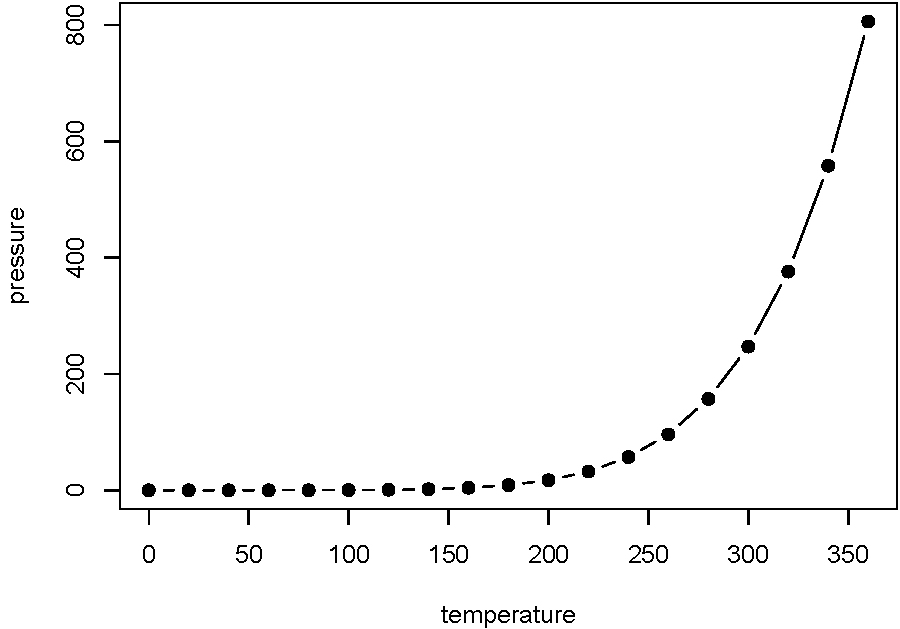
\includegraphics[width=0.7\linewidth]{bookdown-book-zhCN_files/figure-latex/no-caption-1}

这样排版图片的缺点是,如果当前页面没有足够的空间放置图片,图片可能会被放在页面的底部(因此会超出页边空白),或者被推到下一页,在当前页面底部留下一大块空白。这基本上就是 LaTeX 中存在着``浮动环境 (floating environments)''\index{floating environment} 的原因:不能再多个页面上进行拆分(如图片)的元素会被放在浮动环境中,因此它们可以浮动到一个有足够空间容纳它们的页面。但是,向前或向后的浮动也存在着缺点:读者可能需要跳转到另一个页面才能找到当前页面上提到的图片。这只是不得不在多个页面上以固定大小进行排版的一个自然的结果。不过 HTML 中不存在这个问题,因为所有内容都可以被连续地放置在一个页面上(大概有着无限的高度),并且不需要在有着相同页面大小的多个页面上分割任何内容。

如果我们通过区块选项 \texttt{fig.cap} 为代码块分配一个图片标题,那么 R 图形将被放入图形 (figure) 环境中,它将被自动标记和编号,还可以进行交叉引用。图形环境的标签是从代码块的标签生成的。例如,如果块标签是 \texttt{foo},则图片标签将是 \texttt{fig:foo}(前缀 \texttt{fig:} 在 \texttt{foo} 之前添加)。如果要引用一张图片\index{cross-reference},请使用语法 \texttt{\textbackslash{}@ref(label)},\footnote{不要忘记前导的反斜杠!注意 \texttt{ref} 后面的括号 \texttt{()};它们不是大括号 \texttt{\{\}}。},其中 \texttt{label} 是图片标签,例如 \texttt{fig:foo}。

如果要\emph{在图片标题中}利用 Markdown 格式化的优势,需要使用文本引用(请参阅第 \ref{text-references} 节)。例如,当输出格式为 LaTeX/PDF 时,包含 \texttt{\_斜体文本\_} 的图片标题将不起作用,因为下划线是 LaTeX 中的特殊字符。但如果使用文本引用,则当输出为 LaTeX 时,\texttt{\_斜体文本\_} 将被转换为 LaTeX 代码。

\begin{rmdimportant}
如果要交叉引用从代码块生成的图片或表格,请确保块标签仅包含\emph{字母与数字字符 (alphanumber)} (a-z、a-z、0-9)、斜杠 (/) 或破折号 (-)。
\end{rmdimportant}

区块选项 \texttt{fig.asp} 能够被用来设置图片的纵横比。例如图片的高宽比。如果图片的宽度是 6 英寸 (\texttt{fig.width\ =\ 6}) 并且 \texttt{fig.asp\ =\ 0.7},则图片的高度将会自动使用 \texttt{fig.width\ *\ fig.asp\ =\ 6\ *\ 0.7\ =\ 4.2} 计算得出。图 \ref{fig:pressure-plot} 是使用区块选项 \texttt{fig.asp\ =\ 0.7}、\texttt{fig.width\ =\ 6} 和 \texttt{fig.align\ =\ \textquotesingle{}center\textquotesingle{}} 的一个例子,它是从下面的代码中生成的:

\begin{Shaded}
\begin{Highlighting}[]
\FunctionTok{par}\NormalTok{(}\AttributeTok{mar =} \FunctionTok{c}\NormalTok{(}\DecValTok{4}\NormalTok{, }\DecValTok{4}\NormalTok{, .}\DecValTok{1}\NormalTok{, .}\DecValTok{1}\NormalTok{))}
\FunctionTok{plot}\NormalTok{(pressure, }\AttributeTok{pch =} \DecValTok{19}\NormalTok{, }\AttributeTok{type =} \StringTok{\textquotesingle{}b\textquotesingle{}}\NormalTok{)}
\end{Highlighting}
\end{Shaded}

\begin{figure}

{\centering 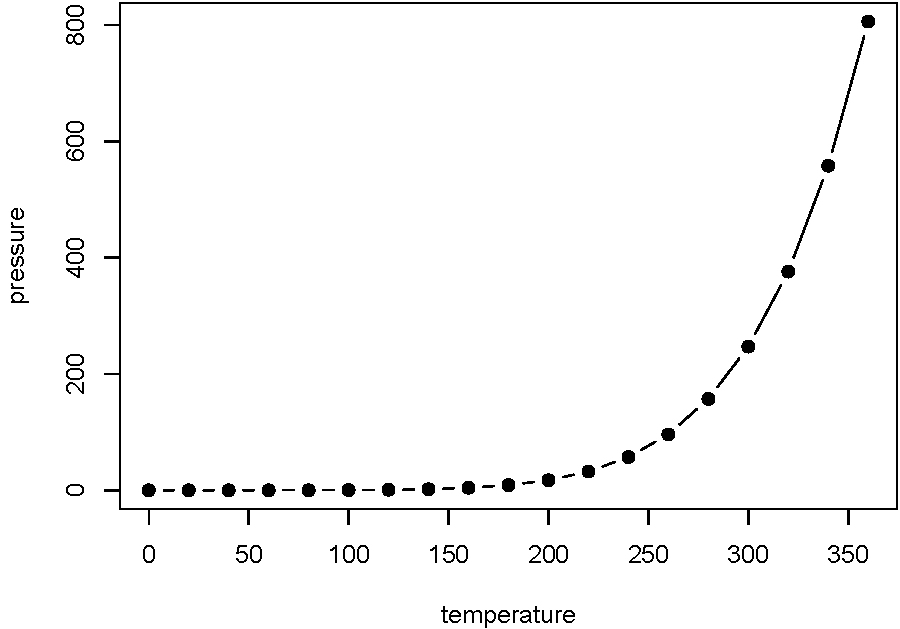
\includegraphics[width=0.9\linewidth]{bookdown-book-zhCN_files/figure-latex/pressure-plot-1} 

}

\caption{指定纵横比、宽度和对齐方式的一个图片示例。}\label{fig:pressure-plot}
\end{figure}

图片的实际大小是由区块选项 \texttt{fig.width} 和 \texttt{fig.height} 决定的(图片的大小由图形设备 (graphical device) 生成),并且我们能够通过区块选项 \texttt{out.width} 和 \texttt{out.height} 指定图片的输出大小。这两个选项可能的取值由文档的输出格式决定。例如,\texttt{out.width\ =\ \textquotesingle{}30\%\textquotesingle{}} 对于 HTML 输出格式来说是有效的,但对于 LaTeX/PDF 输出来说是无效值。然而,\textbf{knitr} 会自动地将 \texttt{x\%} 格式的 \texttt{out.width} 的百分比值转化为 \texttt{(x\ /\ 100)\ \textbackslash{}linewidth}。例如,当输出格式为 LaTeX 时,\texttt{out.width\ =\ \textquotesingle{}70\%\textquotesingle{}} 将会被视为 \texttt{.7\textbackslash{}linewidth}。这样的处理使得我们能够以一致的方式指定图片的相对宽度。图 \ref{fig:cars-plot} 是 \texttt{out.width\ =\ 70\%} 的一个示例。

\begin{Shaded}
\begin{Highlighting}[]
\FunctionTok{par}\NormalTok{(}\AttributeTok{mar =} \FunctionTok{c}\NormalTok{(}\DecValTok{4}\NormalTok{, }\DecValTok{4}\NormalTok{, .}\DecValTok{1}\NormalTok{, .}\DecValTok{1}\NormalTok{))}
\FunctionTok{plot}\NormalTok{(cars, }\AttributeTok{pch =} \DecValTok{19}\NormalTok{)}
\end{Highlighting}
\end{Shaded}

\begin{figure}
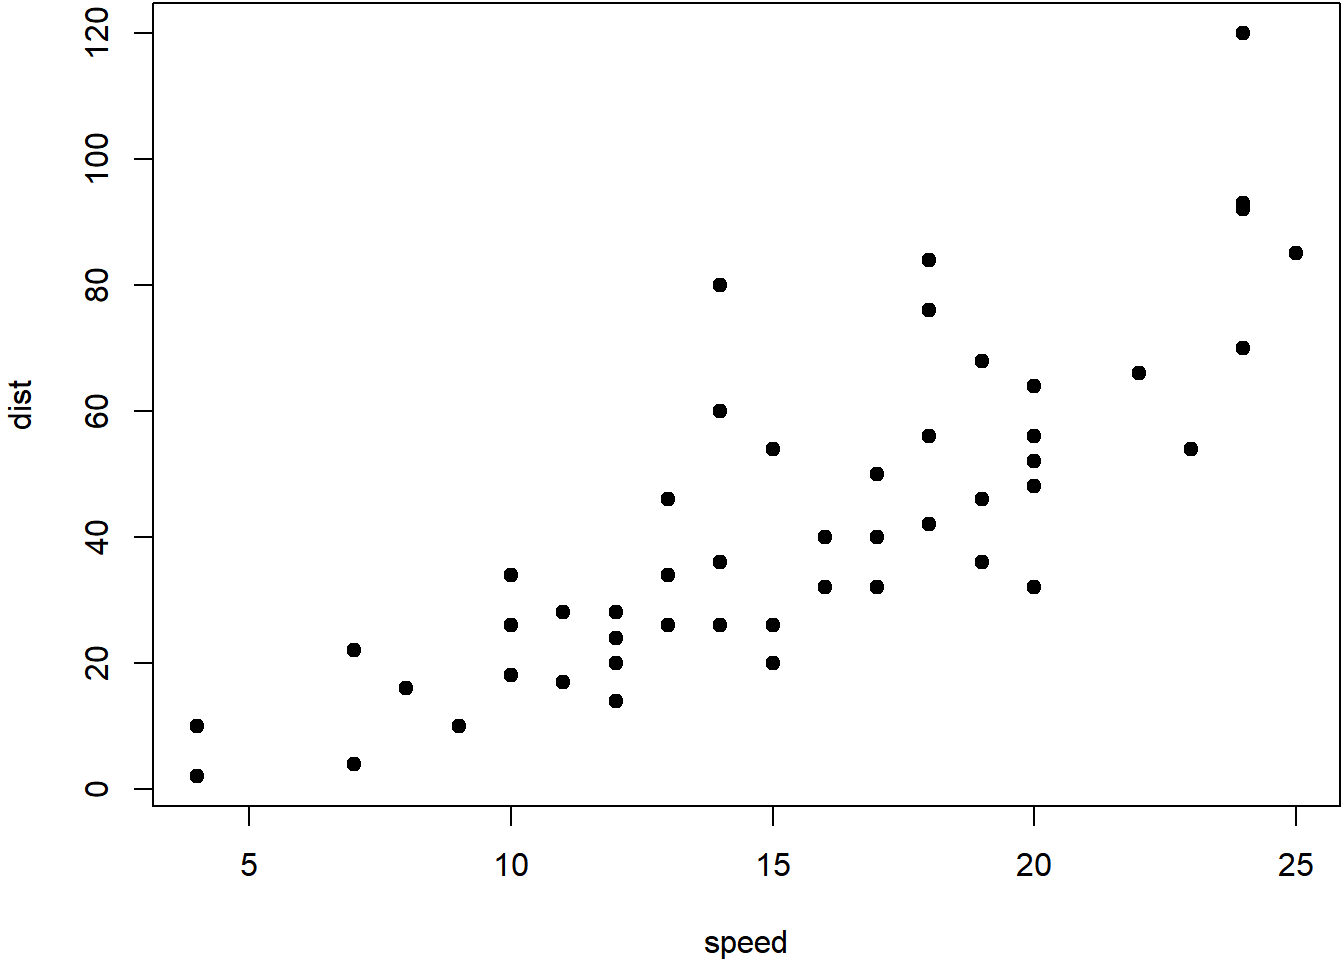
\includegraphics[width=0.7\linewidth]{bookdown-book-zhCN_files/figure-latex/cars-plot-1} \caption{相对宽度为 70\% 的一个图片示例。}\label{fig:cars-plot}
\end{figure}

如果要在一个图形环境中放置多张图片,则必须使用区块选项 \texttt{fig.show\ =\ \textquotesingle{}hold\textquotesingle{}} 来保存代码块中的多张图片,并将它们包含在一个环境中。如果所有图片的宽度之和小于或等于当前线宽 (line width),也可以并排放置图片。例如,如果两张图片具有相同的宽度 \texttt{50\%},则它们将并排放置。类似地,可以通过指定 \texttt{out.width\ =\ \textquotesingle{}33\%\textquotesingle{}} 在一行并排放置三张图片。图 \ref{fig:multi-plots} 是放置两张图的示例,每张图的宽度为 \texttt{50\%}。

\begin{Shaded}
\begin{Highlighting}[]
\FunctionTok{par}\NormalTok{(}\AttributeTok{mar =} \FunctionTok{c}\NormalTok{(}\DecValTok{4}\NormalTok{, }\DecValTok{4}\NormalTok{, .}\DecValTok{1}\NormalTok{, .}\DecValTok{1}\NormalTok{))}
\FunctionTok{plot}\NormalTok{(pressure, }\AttributeTok{pch =} \DecValTok{19}\NormalTok{, }\AttributeTok{type =} \StringTok{\textquotesingle{}b\textquotesingle{}}\NormalTok{)}
\FunctionTok{plot}\NormalTok{(cars, }\AttributeTok{pch =} \DecValTok{19}\NormalTok{)}
\end{Highlighting}
\end{Shaded}

\begin{figure}
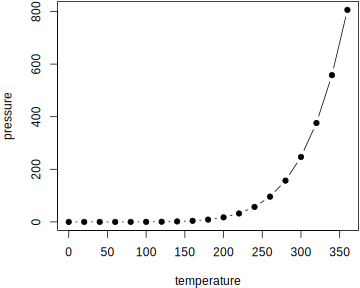
\includegraphics[width=0.5\linewidth]{bookdown-book-zhCN_files/figure-latex/multi-plots-1} 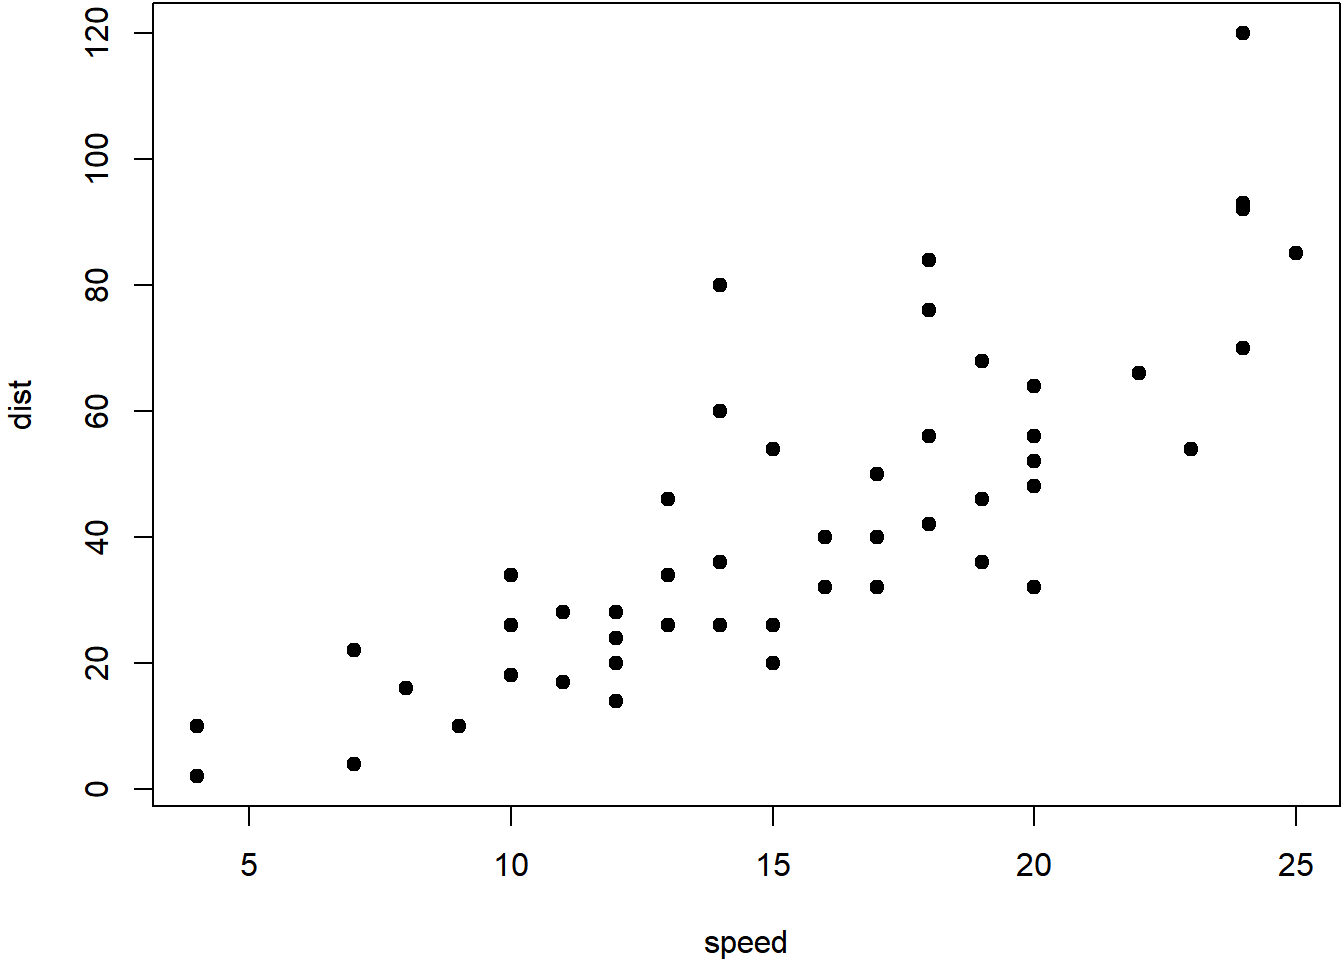
\includegraphics[width=0.5\linewidth]{bookdown-book-zhCN_files/figure-latex/multi-plots-2} \caption{并排放置两张图片。}\label{fig:multi-plots}
\end{figure}

有时,你可能有一些不是从 R 代码生成的图片,这时可以通过函数 \texttt{knitr::include\_graphics()} 将它们包含在 R Markdown 中。图 \ref{fig:knitr-logo} 是在图形环境中包含三个 \textbf{knitr} 徽标的示例。你可以将一个或多个图像路径传递给 \texttt{include\_graphics()}\index{knitr::include\_graphics()} 函数,并且应用于普通 R plots 的所有区块选项也适用于这些图像,例如,可以使用 \texttt{out.width\ =\ \textquotesingle{}33\%\textquotesingle{}} 设置这些图像在输出文档中的宽度。

\begin{Shaded}
\begin{Highlighting}[]
\NormalTok{knitr}\SpecialCharTok{::}\FunctionTok{include\_graphics}\NormalTok{(}\FunctionTok{rep}\NormalTok{(}\StringTok{\textquotesingle{}images/knit{-}logo.png\textquotesingle{}}\NormalTok{, }\DecValTok{3}\NormalTok{))}
\end{Highlighting}
\end{Shaded}

\begin{figure}

\includegraphics[width=0.328\linewidth]{images/knit-logo} 
\includegraphics[width=0.328\linewidth]{images/knit-logo} 
\includegraphics[width=0.328\linewidth]{images/knit-logo} \caption{包含在文档中的来自外部 PNG 图像文件的三个 knitr 徽标。}\label{fig:knitr-logo}
\end{figure}

使用 \texttt{include\_graphics()} 有以下一些优点:

\begin{enumerate}
\def\labelenumi{\arabic{enumi}.}
\tightlist
\item
  你不需要担心文档的输出格式,例如,当输出格式为 LaTeX 时,你可能需要使用 LaTeX 命令 \texttt{\textbackslash{}includegraphics\{\}} 来引入一张图片,而当输出格式是 Markdown 时,你需要使用 \texttt{!{[}{]}()}。\textbf{knitr} 中的 \texttt{include\_graphics()} 函数能够自动处理这些细节。
\item
  控制图像属性的语法与图像是从 R 代码生成时的语法相同,例如,区块选项 \texttt{fig.cap}、\texttt{out.width} 和 \texttt{fig.show} 仍然有着相同的含义。
\item
  \texttt{include\_graphics()} 的表现足够智能,可以在输出格式为 LaTeX 且存在 PDF 图片文件时自动使用 PDF 图片,例如,图片路径 \texttt{foo/bar.png} 能够自动使用 \texttt{foo/bar.pdf} 进行替换(如果后者存在)。在 LaTeX/PDF 输出中,PDF 图片通常比光栅图像具有更好的质量。要使用此功能,请设置参数 \texttt{auto\_pdf\ =\ TRUE},或者设置全局配置项 \texttt{options(knitr.graphics.auto\_pdf\ =\ TRUE)},以便在 R session 中全局启用这个功能。
\item
  你可以使用相同的比例轻松地按比例缩放这些图片。这可以通过 \texttt{dpi} 参数(每英寸像素点数)来完成。默认情况下,该参数从区块选项 \texttt{dpi} 中获取值。如果这个值是数值类型,并且并没有设置区块选项 \texttt{out.width},那么一张图片的输出宽度将会是它的实际宽度(以像素为单位)除以 \texttt{dpi},并且单位变为英寸。例如,对于一张大小为 672 x 480 的图片,在 \texttt{dpi\ =\ 96} 时,它的输出宽度将会是 7 英寸 (\texttt{7in}) 。这个功能需要安装有 \textbf{png} 和/或 \textbf{jpeg} 软件包。通过为区块选项 \texttt{out.width} 提供非空值,或使用 \texttt{include\_graphics(dpi\ =\ NA)},你可以覆盖以英寸为单位的图片宽度的自动计算功能。
\end{enumerate}

\section{表格}\label{tables}

目前来说,生成一个表格\index{table}的最方便的方法是使用函数 \texttt{knitr::kable()},因为在 \textbf{knitr} 中有一些内部技巧可以使其与 \textbf{bookdown} 一起工作,并且用户并不需要知道这些实现细节。我们在本节后面将会解释如何使用其他软件包和函数。

和图片一样,带有标题的表格也将被编号并且可以被引用\index{cross-reference}。\texttt{kable()} 函数将会为表格环境自动生成一个标签,即前缀 \texttt{tab:} 加上区块标签。例如,标签为 \texttt{foo} 的代码块的表格标签将是 \texttt{tab:foo},并且我们仍然能够使用语法 \texttt{\textbackslash{}@ref(label)} 来引用该表格。表 \ref{tab:table-single} 是一个简单的例子。

\begin{Shaded}
\begin{Highlighting}[]
\NormalTok{knitr}\SpecialCharTok{::}\FunctionTok{kable}\NormalTok{(}
  \FunctionTok{head}\NormalTok{(mtcars[, }\DecValTok{1}\SpecialCharTok{:}\DecValTok{8}\NormalTok{], }\DecValTok{10}\NormalTok{), }\AttributeTok{booktabs =} \ConstantTok{TRUE}\NormalTok{,}
  \AttributeTok{caption =} \StringTok{\textquotesingle{}一个包含 mtcars 数据前 10 行的表格。\textquotesingle{}}
\NormalTok{)}
\end{Highlighting}
\end{Shaded}

\begin{table}

\caption{\label{tab:table-single}一个包含 mtcars 数据前 10 行的表格。}
\centering
\begin{tabular}[t]{lrrrrrrrr}
\toprule
  & mpg & cyl & disp & hp & drat & wt & qsec & vs\\
\midrule
Mazda RX4 & 21.0 & 6 & 160.0 & 110 & 3.90 & 2.620 & 16.46 & 0\\
Mazda RX4 Wag & 21.0 & 6 & 160.0 & 110 & 3.90 & 2.875 & 17.02 & 0\\
Datsun 710 & 22.8 & 4 & 108.0 & 93 & 3.85 & 2.320 & 18.61 & 1\\
Hornet 4 Drive & 21.4 & 6 & 258.0 & 110 & 3.08 & 3.215 & 19.44 & 1\\
Hornet Sportabout & 18.7 & 8 & 360.0 & 175 & 3.15 & 3.440 & 17.02 & 0\\
\addlinespace
Valiant & 18.1 & 6 & 225.0 & 105 & 2.76 & 3.460 & 20.22 & 1\\
Duster 360 & 14.3 & 8 & 360.0 & 245 & 3.21 & 3.570 & 15.84 & 0\\
Merc 240D & 24.4 & 4 & 146.7 & 62 & 3.69 & 3.190 & 20.00 & 1\\
Merc 230 & 22.8 & 4 & 140.8 & 95 & 3.92 & 3.150 & 22.90 & 1\\
Merc 280 & 19.2 & 6 & 167.6 & 123 & 3.92 & 3.440 & 18.30 & 1\\
\bottomrule
\end{tabular}
\end{table}

如果要在单个表格环境放入多个表格,请将数据对象(通常是 R 中的数据框)封装到一个列表中有关示例请见表 \ref{tab:table-multi}。请注意此功能仅在 HTML 和 PDF 输出格式中起作用。

\begin{Shaded}
\begin{Highlighting}[]
\NormalTok{knitr}\SpecialCharTok{::}\FunctionTok{kable}\NormalTok{(}
  \FunctionTok{list}\NormalTok{(}
    \FunctionTok{head}\NormalTok{(iris[, }\DecValTok{1}\SpecialCharTok{:}\DecValTok{2}\NormalTok{], }\DecValTok{3}\NormalTok{),}
    \FunctionTok{head}\NormalTok{(mtcars[, }\DecValTok{1}\SpecialCharTok{:}\DecValTok{3}\NormalTok{], }\DecValTok{5}\NormalTok{)}
\NormalTok{  ),}
  \AttributeTok{caption =} \StringTok{\textquotesingle{}两个表格的故事。\textquotesingle{}}\NormalTok{, }\AttributeTok{booktabs =} \ConstantTok{TRUE}
\NormalTok{)}
\end{Highlighting}
\end{Shaded}

\begin{table}
\caption{\label{tab:table-multi}两个表格的故事。}

\centering
\begin{tabular}[t]{rr}
\toprule
Sepal.Length & Sepal.Width\\
\midrule
5.1 & 3.5\\
4.9 & 3.0\\
4.7 & 3.2\\
\bottomrule
\end{tabular}
\centering
\begin{tabular}[t]{lrrr}
\toprule
  & mpg & cyl & disp\\
\midrule
Mazda RX4 & 21.0 & 6 & 160\\
Mazda RX4 Wag & 21.0 & 6 & 160\\
Datsun 710 & 22.8 & 4 & 108\\
Hornet 4 Drive & 21.4 & 6 & 258\\
Hornet Sportabout & 18.7 & 8 & 360\\
\bottomrule
\end{tabular}
\end{table}

当你不希望表格在 PDF 中浮动时,可以使用 LaTeX 软件包 \href{https://www.ctan.org/pkg/longtable}{\textbf{longtable}}\index{longtable},它可以在多个页面上截断一个表格。要使用 \textbf{longtable},请将 \texttt{longtable\ =\ TRUE} 参数传递给 \texttt{kable()},并确保在 LaTeX 导言 (preamble) 中包含 \texttt{\textbackslash{}usepackage\{longtable\}}(有关如何自定义 LaTeX 导言的信息,请参阅第 \ref{yaml-options} 节)。当然,这与 HTML 输出无关,因为 HTML 中的表格并不需要浮动。

\begin{Shaded}
\begin{Highlighting}[]
\NormalTok{knitr}\SpecialCharTok{::}\FunctionTok{kable}\NormalTok{(}
\NormalTok{  iris[}\DecValTok{1}\SpecialCharTok{:}\DecValTok{55}\NormalTok{, ], }\AttributeTok{longtable =} \ConstantTok{TRUE}\NormalTok{, }\AttributeTok{booktabs =} \ConstantTok{TRUE}\NormalTok{,}
  \AttributeTok{caption =} \StringTok{\textquotesingle{}由 longtable 软件包生成的表格。\textquotesingle{}}
\NormalTok{)}
\end{Highlighting}
\end{Shaded}

\begin{longtable}[t]{rrrrl}
\caption{\label{tab:longtable}由 longtable 软件包生成的表格。}\\
\toprule
Sepal.Length & Sepal.Width & Petal.Length & Petal.Width & Species\\
\midrule
5.1 & 3.5 & 1.4 & 0.2 & setosa\\
4.9 & 3.0 & 1.4 & 0.2 & setosa\\
4.7 & 3.2 & 1.3 & 0.2 & setosa\\
4.6 & 3.1 & 1.5 & 0.2 & setosa\\
5.0 & 3.6 & 1.4 & 0.2 & setosa\\
\addlinespace
5.4 & 3.9 & 1.7 & 0.4 & setosa\\
4.6 & 3.4 & 1.4 & 0.3 & setosa\\
5.0 & 3.4 & 1.5 & 0.2 & setosa\\
4.4 & 2.9 & 1.4 & 0.2 & setosa\\
4.9 & 3.1 & 1.5 & 0.1 & setosa\\
\addlinespace
5.4 & 3.7 & 1.5 & 0.2 & setosa\\
4.8 & 3.4 & 1.6 & 0.2 & setosa\\
4.8 & 3.0 & 1.4 & 0.1 & setosa\\
4.3 & 3.0 & 1.1 & 0.1 & setosa\\
5.8 & 4.0 & 1.2 & 0.2 & setosa\\
\addlinespace
5.7 & 4.4 & 1.5 & 0.4 & setosa\\
5.4 & 3.9 & 1.3 & 0.4 & setosa\\
5.1 & 3.5 & 1.4 & 0.3 & setosa\\
5.7 & 3.8 & 1.7 & 0.3 & setosa\\
5.1 & 3.8 & 1.5 & 0.3 & setosa\\
\addlinespace
5.4 & 3.4 & 1.7 & 0.2 & setosa\\
5.1 & 3.7 & 1.5 & 0.4 & setosa\\
4.6 & 3.6 & 1.0 & 0.2 & setosa\\
5.1 & 3.3 & 1.7 & 0.5 & setosa\\
4.8 & 3.4 & 1.9 & 0.2 & setosa\\
\addlinespace
5.0 & 3.0 & 1.6 & 0.2 & setosa\\
5.0 & 3.4 & 1.6 & 0.4 & setosa\\
5.2 & 3.5 & 1.5 & 0.2 & setosa\\
5.2 & 3.4 & 1.4 & 0.2 & setosa\\
4.7 & 3.2 & 1.6 & 0.2 & setosa\\
\addlinespace
4.8 & 3.1 & 1.6 & 0.2 & setosa\\
5.4 & 3.4 & 1.5 & 0.4 & setosa\\
5.2 & 4.1 & 1.5 & 0.1 & setosa\\
5.5 & 4.2 & 1.4 & 0.2 & setosa\\
4.9 & 3.1 & 1.5 & 0.2 & setosa\\
\addlinespace
5.0 & 3.2 & 1.2 & 0.2 & setosa\\
5.5 & 3.5 & 1.3 & 0.2 & setosa\\
4.9 & 3.6 & 1.4 & 0.1 & setosa\\
4.4 & 3.0 & 1.3 & 0.2 & setosa\\
5.1 & 3.4 & 1.5 & 0.2 & setosa\\
\addlinespace
5.0 & 3.5 & 1.3 & 0.3 & setosa\\
4.5 & 2.3 & 1.3 & 0.3 & setosa\\
4.4 & 3.2 & 1.3 & 0.2 & setosa\\
5.0 & 3.5 & 1.6 & 0.6 & setosa\\
5.1 & 3.8 & 1.9 & 0.4 & setosa\\
\addlinespace
4.8 & 3.0 & 1.4 & 0.3 & setosa\\
5.1 & 3.8 & 1.6 & 0.2 & setosa\\
4.6 & 3.2 & 1.4 & 0.2 & setosa\\
5.3 & 3.7 & 1.5 & 0.2 & setosa\\
5.0 & 3.3 & 1.4 & 0.2 & setosa\\
\addlinespace
7.0 & 3.2 & 4.7 & 1.4 & versicolor\\
6.4 & 3.2 & 4.5 & 1.5 & versicolor\\
6.9 & 3.1 & 4.9 & 1.5 & versicolor\\
5.5 & 2.3 & 4.0 & 1.3 & versicolor\\
6.5 & 2.8 & 4.6 & 1.5 & versicolor\\
\bottomrule
\end{longtable}

Pandoc 支持多种类型的 \href{http://pandoc.org/MANUAL.html\#tables}{Markdown 表格},例如简单表格、多行表格、栅格表格和管道表格。\texttt{knitr::kable()} 生成的是这样一个简单的表格:

\begin{Shaded}
\begin{Highlighting}[]
\NormalTok{Table:Markdown 的一个简单表格。}

\NormalTok{ Sepal.Length   Sepal.Width   Petal.Length   Petal.Width}
\NormalTok{{-}{-}{-}{-}{-}{-}{-}{-}{-}{-}{-}{-}{-}  {-}{-}{-}{-}{-}{-}{-}{-}{-}{-}{-}{-}  {-}{-}{-}{-}{-}{-}{-}{-}{-}{-}{-}{-}{-}  {-}{-}{-}{-}{-}{-}{-}{-}{-}{-}{-}{-}}
\InformationTok{          5.1           3.5            1.4           0.2}
\InformationTok{          4.9           3.0            1.4           0.2}
\InformationTok{          4.7           3.2            1.3           0.2}
\InformationTok{          4.6           3.1            1.5           0.2}
\InformationTok{          5.0           3.6            1.4           0.2}
\InformationTok{          5.4           3.9            1.7           0.4}
\end{Highlighting}
\end{Shaded}

你可以在文档中使用任何类型的 Markdown 表格。为了能够交叉引用 Markdown 表格,它必须具有 \texttt{Table:\ (\textbackslash{}\#label)\ Caption\ here} 格式的标签标题,其中 \texttt{label} 必须具有前缀 \texttt{tab:},例如 \texttt{tab:simple-table}。

如果决定使用其它 R 软件包生成表格,则必须确保表格环境的标签以 \texttt{(\textbackslash{}\#label)} 的格式出现在表格标题的开头(同样地,\texttt{label} 必须具有前缀 \texttt{tab:})。你必须非常小心表格生成函数的 \emph{通用性}:它应该在 HTML 和 LaTeX 输出格式下能够自动正常工作,因此必须在内部考虑输出格式(检查 \texttt{knitr::opts\_knit\$get(\textquotesingle{}rmarkdown.pandoc.to\textquotesingle{})})。当输出 HTML 表格时,标题必须写在 \texttt{\textless{}caption\textgreater{}\textless{}/caption\textgreater{}} 标签中,不过对于简单的表格,\texttt{kable()} 就足够了。如果你需要创建复杂的表格(例如,某些单元格跨越多列/行),则必须考虑上述问题。

\section{交叉引用}\label{cross-references}

我们已经解释了交叉引用\index{cross-reference}是如何在方程(第 \ref{equations} 节)、定理(第 \ref{theorems} 节)、图片(第 \ref{figures} 节)和表格(第 \ref{tables} 节)上起作用的。事实上,你也能够使用相同的语法 \texttt{\textbackslash{}@ref(label)} 引用章节,在此时 \texttt{label} 是章节的标识符。默认情况下,Pandoc 将会为全部章节标题生成一个标识符,例如 \texttt{\#\ Hello\ World} 这一章将会有名为 \texttt{hello-world} 的标识符。我们建议你手动为章节标题指定标识符,以确保更改章节标题后不会忘记更新参考标签。要将标识符分配给章节标题,只需要简单的在章节标题之后添加 \texttt{\{\#id\}} 即可。章节标题的其他属性可以使用标准 \href{http://pandoc.org/MANUAL.html\#heading-identifiers}{Pandoc 语法}。

当找不到引用的标签时,你将会看见两个问号 \ref{fig:does-not-exist}以及编译书籍时在 R console 中打印的警告信息。

你也可以使用显式或自动指定的章节标识符,甚至是实际的章节标题文本创建基于文本的章节链接。

\begin{itemize}
\tightlist
\item
  如果你对使用章节标题作为链接文本感到满意,请在一组方括号内使用它:

  \begin{itemize}
  \tightlist
  \item
    \texttt{{[}章节标题文本{]}}: 例如通过 \texttt{{[}单个文档{]}} 创建指定的链接文本 ``\hyperref[a-single-document]{单个文档}''
  \end{itemize}
\item
  如果要指定自定义链接文本,有两种方法:

  \begin{itemize}
  \tightlist
  \item
    \texttt{{[}链接文本{]}{[}章节标题文本{]}}。例如,``\hyperref[internationalization]{非英语书籍}'' via \texttt{{[}非英语书籍{]}{[}国际化{]}}
  \item
    \texttt{{[}链接文本{]}(\#标识符)}。例如,``\hyperref[tables]{表格填充}'' via \texttt{{[}表格填充{]}(\#tables)}
  \end{itemize}
\end{itemize}

Pandoc 文档提供了更多详细信息,请见 \href{http://pandoc.org/MANUAL.html\#extension-auto_identifiers}{自动指定章节标识符 (automatic section IDs)} 和 \href{http://pandoc.org/MANUAL.html\#extension-implicit_header_references}{隐式标题引用 (implicit header references)}。

当我们在 PDF 或 HTML 输出文档下提及并不在当前页面的文档项目时,交叉引用仍然能够起作用。例如,请见方程 \eqref{eq:binom} 和图片 \ref{fig:knitr-logo}。

\section{自定义区块}\label{ux81eaux5b9aux4e49ux533aux5757}

自定义区块通常用于技术书籍中,它可以创建引起读者注意的代码和/或描述文字的突出文本框。例如,自定义区块可用于高亮显示注释或警告。可以使用 Pandoc 的 \texttt{Div} 围栏区块 (\url{https://pandoc.org/MANUAL.html\#divs-and-spans}) 的语法将其包含在多个 \textbf{bookdown} 输出格式中。关于其用法可以阅读 \href{https://bookdown.org/yihui/rmarkdown-cookbook/custom-blocks.html}{\emph{R Markdown Cookbook}} 第 9.6 节 \citep{rmarkdown2020}。

HTML 输出格式 \texttt{bs4\_book()} 包括为选定的自定义区块设置样式的功能,请见第 \ref{bs4-book} 节。

\section{引文}\label{citations}

Pandoc 提供了两种方法来管理文档中引用文献\index{citation}和参考书目。

\begin{enumerate}
\def\labelenumi{\arabic{enumi}.}
\item
  默认的方法是使用名为 \href{https://github.com/jgm/pandoc-citeproc}{\texttt{pandoc-citeproc}} 的 Pandoc 帮助程序,它遵循 \href{https://docs.citationstyles.org/en/v1.0.1/specification.html}{引用样式语言 (Citation Style Language, CSL)} 的规范,并从大量可用的 \href{https://www.zotero.org/styles/}{CSL 样式文件 (CSL style files)} 之一中获取特定的格式说明。
\item
  用户也可以选择使用 \href{https://ctan.org/pkg/natbib}{\textbf{natbib}}(基于 \texttt{bibtex})或 \href{https://ctan.org/pkg/biblatex}{\textbf{biblatex}} 作为``引文软件包''。在这种情况下,参考书目数据文件需要为 \texttt{bibtex} 或 \texttt{biblatex} 格式,并且文档输出格式仅限于 PDF。与 CSL 相同,可用地参考书目样式也有许多(请参阅这些软件包的文档)。

  为了使用 \textbf{natbib} 或 \textbf{biblatex} 处理参考文献,你可用设置 R Markdown 输出格式的 \texttt{citation\_package} 选项,例如:

\begin{Shaded}
\begin{Highlighting}[]
\FunctionTok{output}\KeywordTok{:}
\AttributeTok{  }\FunctionTok{pdf\_document}\KeywordTok{:}
\AttributeTok{    }\FunctionTok{citation\_package}\KeywordTok{:}\AttributeTok{ natbib}
\AttributeTok{  bookdown:}\FunctionTok{:pdf\_book}\KeywordTok{:}
\AttributeTok{    }\FunctionTok{citation\_package}\KeywordTok{:}\AttributeTok{ biblatex}
\end{Highlighting}
\end{Shaded}
\end{enumerate}

即使你为 PDF 输出格式选择了 \texttt{natbib} 或 \texttt{biblatex} 作为引文软件包,所有其它输出格式都将使用 \texttt{pandoc-citeproc}。如果使用相匹配的样式(例如对于 \texttt{biblatex} 采用 \texttt{biblio-style:\ apa},而对于 \texttt{pandoc-citeproc} 采用 \texttt{csl:\ apa.csl}),输出到 PDF 和 非 PDF 的格式将非常相似,但不一定是相同的。

对于任何非 PDF 输出格式,\texttt{pandoc-citeproc} 是唯一可用的选项。如果 PDF 和非 PDF 输出格式之间的一致性很重要,请始终使用 \texttt{pandoc-citeproc}。

参考书目数据有很多种格式。本节仅展示了 BibTeX 数据库的示例,对于其他格式请参见 Pandoc 使用指南中 \href{https://pandoc.org/MANUAL.html\#citations}{``Citations''} 一节。

BibTeX 数据库是一个纯文本文件(依惯例其文件扩展名为 \texttt{.bib}),其内容包含有类似于以下所示的参考书目条目:

\begin{Shaded}
\begin{Highlighting}[]
\VariableTok{@Manual}\NormalTok{\{}\OtherTok{R}\NormalTok{{-}}\OtherTok{base}\NormalTok{,}
  \DataTypeTok{title}\NormalTok{ = \{R: A Language and Environment for Statistical}
\NormalTok{    Computing\},}
  \DataTypeTok{author}\NormalTok{ = \{\{R Core Team\}\},}
  \DataTypeTok{organization}\NormalTok{ = \{R Foundation for Statistical Computing\},}
  \DataTypeTok{address}\NormalTok{ = \{Vienna, Austria\},}
  \DataTypeTok{year}\NormalTok{ = \{2016\},}
  \DataTypeTok{url}\NormalTok{ = \{https://www.R{-}project.org/\},}
\NormalTok{\}}
\end{Highlighting}
\end{Shaded}

参考书目条目以 \texttt{@type\{} 开头,其中 \texttt{type} 可以是 \texttt{article}、\texttt{book}、\texttt{manual}等等。\footnote{类型名称不区分大小写,因此不管是 \texttt{manual}、\texttt{Manual} 或 \texttt{MANUAL} 都可以。}紧跟着是一个引文关键词,在上面的示例中为 \texttt{R-base}。要引用一个条目,需要使用 \texttt{@key} 或 \texttt{{[}@key{]}}(后者会将引用文字放在圆括号中),例如,\texttt{@R-base} 被渲染为 \citet{R-base},而 \texttt{{[}@R-base{]}} 则渲染为 ``\citep{R-base}''。注释也可以包含在方括号中,例如 \texttt{{[}a\ note\ about,\ @R-base{]}} 将会被渲染为 ``\citep[a note about,][]{R-base}''。如果你对 LaTeX 中的 \textbf{natbib} 软件包很熟悉,你会发现 \texttt{@key} 基本上就是 \texttt{\textbackslash{}citet\{key\}},而 \texttt{{[}@key{]}} 等同于 \texttt{\textbackslash{}citep\{key\}}。

在一个参考书目条目中有许多字段,例如 \texttt{title}、\texttt{author} 和 \texttt{year} 等。你可用在 \url{https://en.wikipedia.org/wiki/BibTeX} 查看 BibTeX 中可能的条目和字段类型。

在 \textbf{knitr} 中有一个帮助函数 \texttt{write\_bib()},它能够为 R 软件包自动生成 BibTeX 条目,例如:

\begin{Shaded}
\begin{Highlighting}[]
\CommentTok{\# the second argument can be a .bib file}
\NormalTok{knitr}\SpecialCharTok{::}\FunctionTok{write\_bib}\NormalTok{(}\FunctionTok{c}\NormalTok{(}\StringTok{\textquotesingle{}knitr\textquotesingle{}}\NormalTok{, }\StringTok{\textquotesingle{}stringr\textquotesingle{}}\NormalTok{), }\StringTok{\textquotesingle{}\textquotesingle{}}\NormalTok{, }\AttributeTok{width =} \DecValTok{60}\NormalTok{)}
\end{Highlighting}
\end{Shaded}

\begin{verbatim}
@Manual{R-knitr,
  title = {knitr: A General-Purpose Package for Dynamic
    Report Generation in R},
  author = {Yihui Xie},
  year = {2023},
  note = {R package version 1.45},
  url = {https://yihui.org/knitr/},
}

@Manual{R-stringr,
  title = {stringr: Simple, Consistent Wrappers for Common
    String Operations},
  author = {Hadley Wickham},
  year = {2023},
  note = {R package version 1.5.1,
    https://github.com/tidyverse/stringr},
  url = {https://stringr.tidyverse.org},
}

@Book{knitr2015,
  title = {Dynamic Documents with {R} and knitr},
  author = {Yihui Xie},
  publisher = {Chapman and Hall/CRC},
  address = {Boca Raton, Florida},
  year = {2015},
  edition = {2nd},
  note = {ISBN 978-1498716963},
  url = {https://yihui.org/knitr/},
}

@InCollection{knitr2014,
  booktitle = {Implementing Reproducible Computational
    Research},
  editor = {Victoria Stodden and Friedrich Leisch and Roger
    D. Peng},
  title = {knitr: A Comprehensive Tool for Reproducible
    Research in {R}},
  author = {Yihui Xie},
  publisher = {Chapman and Hall/CRC},
  year = {2014},
  note = {ISBN 978-1466561595},
}
\end{verbatim}

一旦你有一个或多个 \texttt{.bib} 文件,你可以在第一个 R Markdown 文档(通常是 \texttt{index.Rmd})中的 YAML 元数据中使用字段 \texttt{bibliography} 来使用它们,你也可以通过 \texttt{biblio-style} 指定参考书目样式(它仅对 PDF 输出文档起作用),例如:

\begin{Shaded}
\begin{Highlighting}[]
\PreprocessorTok{{-}{-}{-}}
\FunctionTok{bibliography}\KeywordTok{:}\AttributeTok{ }\KeywordTok{[}\StringTok{"one.bib"}\KeywordTok{,}\AttributeTok{ }\StringTok{"another.bib"}\KeywordTok{,}\AttributeTok{ }\StringTok{"yet{-}another.bib"}\KeywordTok{]}
\FunctionTok{biblio{-}style}\KeywordTok{:}\AttributeTok{ }\StringTok{"apalike"}
\FunctionTok{link{-}citations}\KeywordTok{:}\AttributeTok{ }\CharTok{true}
\PreprocessorTok{{-}{-}{-}}
\end{Highlighting}
\end{Shaded}

字段 \texttt{link-citations} 能够用来添加从``作者-年份''格式的引文文本到 HTML 输出中参考书目条目的内部链接。

当输出格式为 LaTeX 时,参考文献列表将自动放在文档末尾的章节中。对于非 LaTeX 输出,你可以为你的书籍添加一个空章节作为最后一章。例如,如果最后一章是 Rmd 文件 \texttt{06-references.Rmd},则它的内容可以是内联 R 表达式:

\begin{Shaded}
\begin{Highlighting}[]
\InformationTok{\textasciigrave{}r if (knitr::is\_html\_output()) \textquotesingle{}\# References \{{-}\}\textquotesingle{}\textasciigrave{}}
\end{Highlighting}
\end{Shaded}

有关如何使用引文的更多详细说明和示例,请参阅 Pandoc 使用指南的``引文''部分。

\section{索引}\label{latex-index}

目前只有 LaTeX/PDF 输出支持索引\index{index}。要在书籍之后打印索引,你可以在 LaTeX 导言 (preamble) 中使用 LaTeX 软件包 \textbf{makeidx} (请参阅第 \ref{yaml-options} 节):

\begin{Shaded}
\begin{Highlighting}[]
\BuiltInTok{\textbackslash{}usepackage}\NormalTok{\{}\ExtensionTok{makeidx}\NormalTok{\}}
\FunctionTok{\textbackslash{}makeindex}
\end{Highlighting}
\end{Shaded}

或者,你也可以使用 \textbf{imakeidx} 软件包:

\begin{Shaded}
\begin{Highlighting}[]
\BuiltInTok{\textbackslash{}usepackage}\NormalTok{\{}\ExtensionTok{imakeidx}\NormalTok{\}}
\end{Highlighting}
\end{Shaded}

这个软件包提供了格式化索引的额外功能,例如:

\begin{Shaded}
\begin{Highlighting}[]
\FunctionTok{\textbackslash{}makeindex}\NormalTok{[intoc=true,columns=3,columnseprule=true,}
\NormalTok{           options={-}s latex/indexstyles.ist]}
\end{Highlighting}
\end{Shaded}

在上面的例子中,\texttt{intoc=true} 将在目录中包含一个索引条目,\texttt{columns=3} 将把索引格式转为三列,\texttt{columnseprule=true} 将在相邻的索引列之间显示一条线。最后,\texttt{options=-s\ latex/indexstyles.ist} 将使用位于 \texttt{latex/indexstyles.ist} 的索引样式文件中包含的额外格式化选项。\textbf{imakeidx} 软件包中还有许多其他的功能,请参阅其文档以了解更多细节。

\subsection{插入索引条目}\label{ux63d2ux5165ux7d22ux5f15ux6761ux76ee}

索引条目可以通过在书籍正文中使用 \texttt{\textbackslash{}index\{\}} 命令创建,例如:

\begin{Shaded}
\begin{Highlighting}[]
\NormalTok{Version Control}\FunctionTok{\textbackslash{}index}\NormalTok{\{Version Control\} is an}
\NormalTok{important component of the SDLC.}
\end{Highlighting}
\end{Shaded}

类似的,可以为某项插入一个子条目:

\begin{verbatim}
Git\index{Version Control!Git} is a
popular version control system.
\end{verbatim}

上面的例子将会在索引的 ``Version Control'' 下方添加一个 ``Git'' 条目。

要创建一个出现在项目子条目底部的 ``see also'' 条目(没有页码),首先在 LaTex 导言 (preamble) 文件中调用 \texttt{\textbackslash{}makeindex} 的下方添加如下内容:

\begin{Shaded}
\begin{Highlighting}[]
\CommentTok{\% to create a "see also" that appears at the bottom of the}
\CommentTok{\% subentries and with no page number, do the following:}
\CommentTok{\% \textbackslash{}index\{Main entry!zzzzz@\textbackslash{}igobble|seealso\{Other item\}\}}

\FunctionTok{\textbackslash{}newcommand}\NormalTok{\{}\ExtensionTok{\textbackslash{}ii}\NormalTok{\}[1]\{\{}\FunctionTok{\textbackslash{}it}\NormalTok{ \#1\}\}}
\FunctionTok{\textbackslash{}newcommand}\NormalTok{\{}\ExtensionTok{\textbackslash{}nn}\NormalTok{\}[1]\{\#1n\}}

\FunctionTok{\textbackslash{}def\textbackslash{}igobble}\NormalTok{\#1\{\}}
\end{Highlighting}
\end{Shaded}

然后,在你的书籍中使用 \texttt{\textbackslash{}index\{Main\ entry!zzzzz@\textbackslash{}igobble\textbar{}seealso\{Other\ item\}\}} 语法。 举个例子:

\begin{Shaded}
\begin{Highlighting}[]
\NormalTok{Backups}\FunctionTok{\textbackslash{}index}\NormalTok{\{Version Control!zzzzz@}\FunctionTok{\textbackslash{}igobble}\NormalTok{|seealso\{backups\}\}}
\NormalTok{should be part of your version control system.}
\end{Highlighting}
\end{Shaded}

\subsection{构建索引}\label{ux6784ux5efaux7d22ux5f15}

要构建索引,可以通过 YAML 选项 \texttt{includes\ -\textgreater{}\ after\_body} 在书籍末尾插入 \texttt{\textbackslash{}printindex}。

\section{HTML 小组件}\label{html-ux5c0fux7ec4ux4ef6}

尽管 R 的最大优势之一是数据可视化,但仍然有大量 JavaScript 库可用于更丰富的数据可视化。这些库可以被用来构建能够在 Web 浏览器中轻松呈现的可交互式应用,因此用户不必安装其它任何软件包就能够查看可视化效果。将这些 JavaScript 库引入 R 的一种方法是通过 \href{http://htmlwidgets.org}{\textbf{htmlwidgets}} 软件包 \citep{R-htmlwidgets}\index{HTML widget}。

HTML 小组件能够呈现为独立的网页(就像 R plot 一样),或者嵌入 R Markdown 文档和 Shiny 应用中。它们最初仅被设计用于 HTML 输出,并且需要使用 JavaScript,因此它们不能用于非 HTML 输出格式,例如 LaTeX/PDF。在 \textbf{knitr} v1.13 之前,如果你试图在非 HTML 输出格式中呈现 HTML 小组件,你将会收到错误消息。从 \textbf{knitr} v1.13 开始,HTML 小组件将会自动被呈现为通过 \textbf{webshot} 软件包 \citep{R-webshot} 截取的屏幕截图。当然,你需要安装有 \textbf{webshot} 软件包。另外,你必须安装 PhantomJS (\url{http://phantomjs.org}),因为 \textbf{webshot} 使用它来捕捉屏幕截图。\textbf{webshot} 和 PhantomJS 都能够在 R 中自动安装:

\begin{Shaded}
\begin{Highlighting}[]
\FunctionTok{install.packages}\NormalTok{(}\StringTok{\textquotesingle{}webshot\textquotesingle{}}\NormalTok{)}
\NormalTok{webshot}\SpecialCharTok{::}\FunctionTok{install\_phantomjs}\NormalTok{()}
\end{Highlighting}
\end{Shaded}

函数 \texttt{install\_phantomjs()} 适用于 Windows、OS X 和 Linux。如果你熟悉修改系统环境变量 \texttt{PATH},也可以选择自己下载和安装 PhantomJS。

当 \textbf{knitr} 在代码块中检测到 HTML 小组件对象时,它要么在当前输出格式为 HTML 时正常呈现小组件,要么在输出格式不是 HTML 时将小组件保存为 HTML 页面,并调用 \textbf{webshot} 来捕获 HTML 页面的屏幕图像。下面是从 \textbf{DT} 软件包 \citep{R-DT} 创建的表格的示例:

\begin{Shaded}
\begin{Highlighting}[]
\NormalTok{DT}\SpecialCharTok{::}\FunctionTok{datatable}\NormalTok{(iris)}
\end{Highlighting}
\end{Shaded}

\begin{figure}
\centering
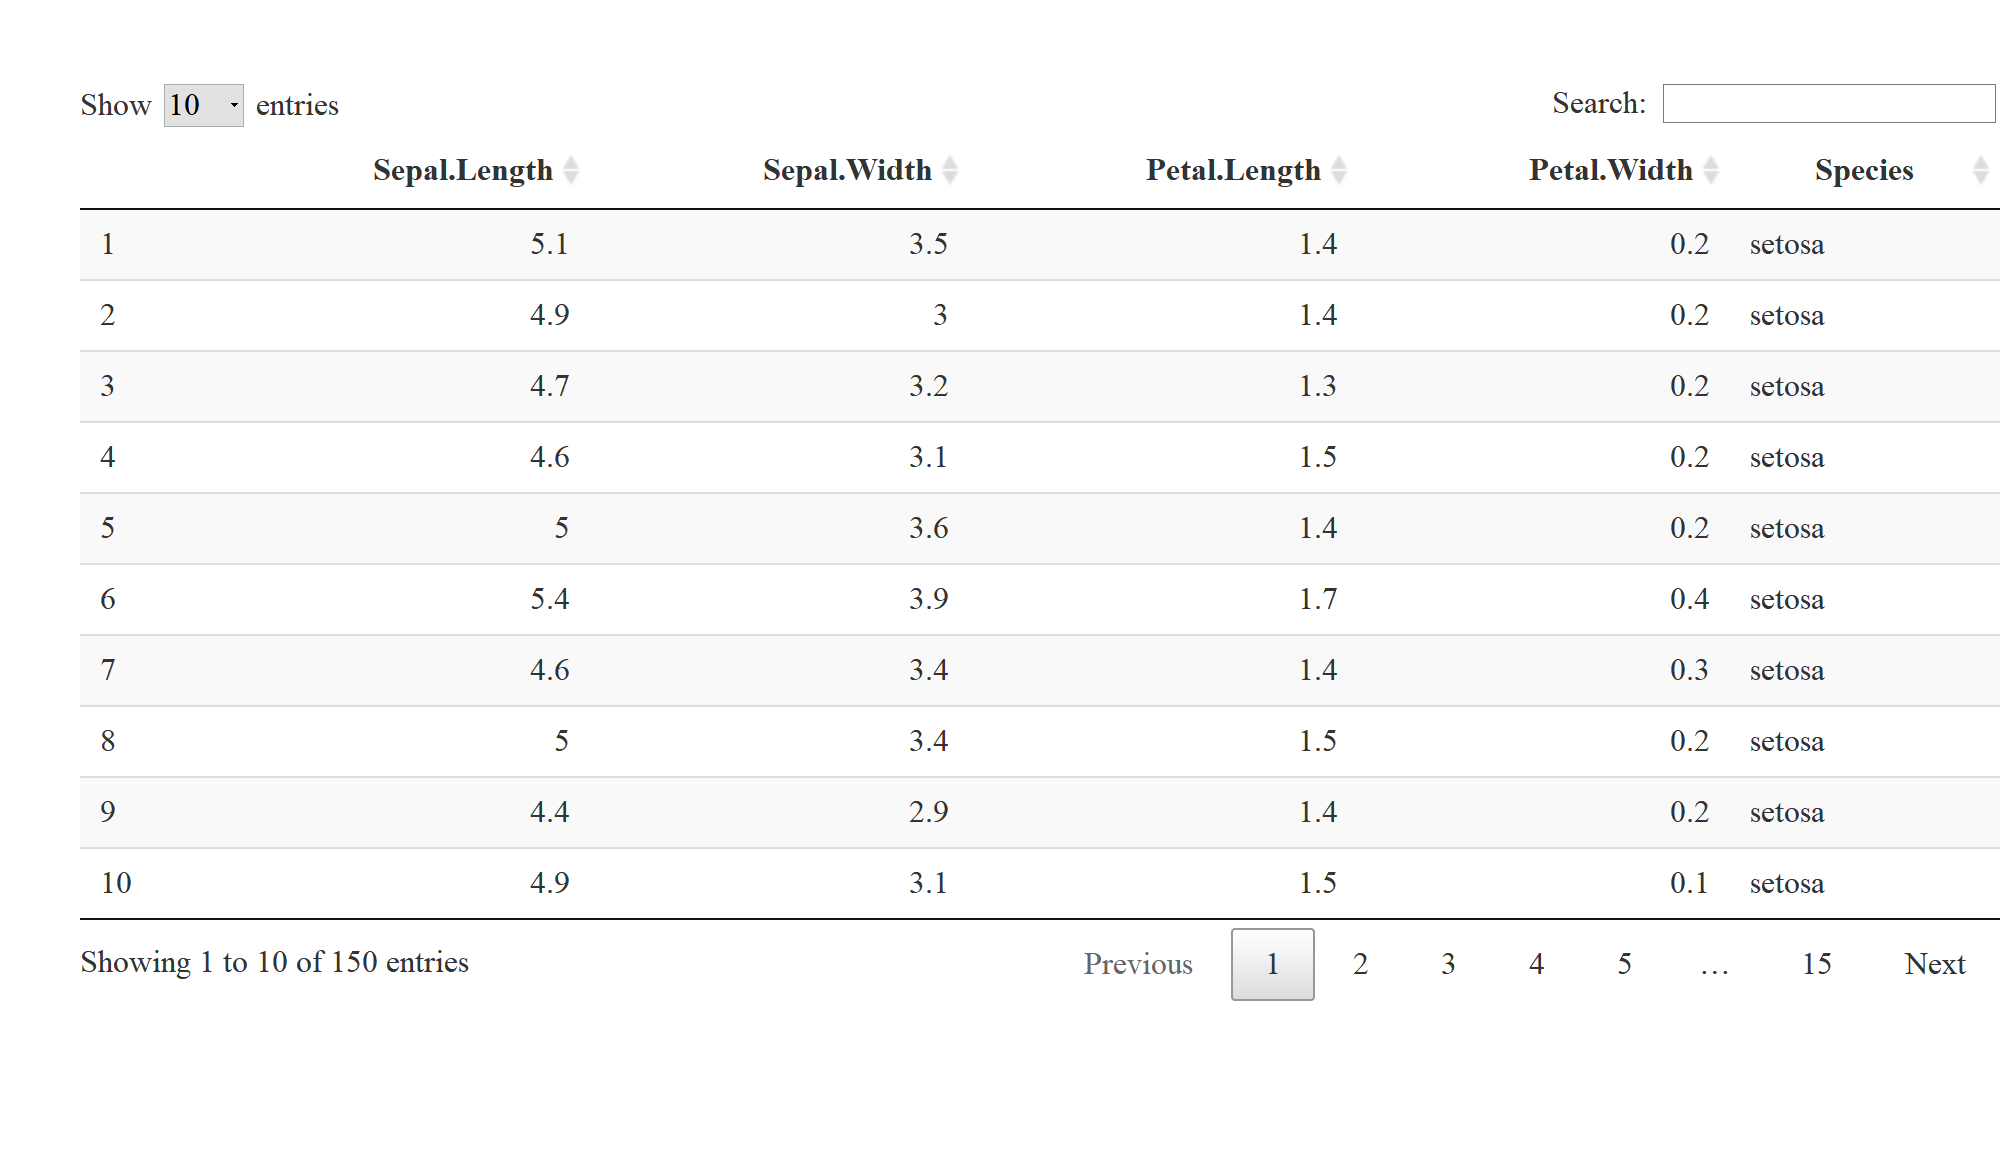
\includegraphics{bookdown-book-zhCN_files/figure-latex/DT-demo-1.png}
\caption{\label{fig:DT-demo}A table widget rendered via the DT package.}
\end{figure}

如果你现在以网页的形式阅读本书,应该能看到由上述代码块生成的交互式表格:你可以对列进行排序并在表格中进行搜索。如果你正在阅读本书的非 HTML 版本,应该能看到这个表格的屏幕截图。由于真实的 Web 浏览器和 PhantomJS 的虚拟浏览器之间的差异,屏幕截图可能与 Web 浏览器中呈现的实际小组件略有不同。

有许多与屏幕捕获相关的 \textbf{knitr} 区块选项。第一,如果你对自动截图的质量不满意,或者想要一个特定状态的小组件的屏幕截图(例如在你单击并排序表的某一列之后),可以手动捕获屏幕图像,并通过区块选项 \texttt{screenshot.alt}(备选屏幕截图 (alternative screenshots))提供自己的屏幕截图。该选项使用图像的路径获得图片。如果一个区块中有多个小组件,则可以提供一个图像路径的向量。当该选项存在时,\textbf{knitr} 将不再调用 \textbf{webshot} 自动截图。

第二,有时你可能希望强制 \textbf{knitr} 使用静态屏幕截图,而不是在 HTML 页面上呈现实际的小组件。在这种情况下,你可以设置区块选项 \texttt{screenshot.force\ =\ TRUE}。小组件将始终呈现为静态图像。请注意,你仍然可以选择使用自动或自定义的屏幕截图。

第三,\textbf{webshot} 有一些控制自动屏幕截图的选项,你可以通过区块选项 \texttt{screenshot.opts} 来进行设置,该选项接收一个类似 \texttt{list(delay\ =\ 2,\ cliprect\ =\ \textquotesingle{}viewport\textquotesingle{})} 的列表。有关可用选项的完整列表,请查阅帮助页面 \href{https://wch.github.io/webshot/reference/webshot.html}{\texttt{?webshot::webshot}},而其中一些选项的效果说明请见\href{https://wch.github.io/web/packages/webshot/articles/intro.html}{软件包介绍}。这里的 \texttt{delay} 选项对于需要很长时间进行渲染的小组件来说很重要:\texttt{delay} 指定了 PhantomJS 在截图前等待的秒数。如果看到不完整的屏幕截图,可能需要指定更长的延迟时间(默认值为 0.2 秒)。

第四,如果你觉得捕获屏幕截图很慢,或者不想每次执行代码块时都这样做,可以使用区块选项 \texttt{cache\ =\ TRUE} 来缓存区块。缓存对于 HTML 和非 HTML 输出格式都适用。

屏幕截图的表现类似于普通的 R plot,因为许多与图形相关的区块选项也适用于屏幕截图,包括 \texttt{fig.width}、\texttt{fig.height}、\texttt{out.width}、\texttt{fig.cap} 等。因此你可以在输出文档中指定屏幕截图的大小,并为其指定图片标题。可以通过区块选项 \texttt{dev} 指定自动截图的图片格式,可能的值为 \texttt{pdf}、\texttt{png} 和 \texttt{jpeg}。PDF 输出的默认值为 \texttt{pdf},其他类型输出的默认值为 \texttt{png}。请注意,\texttt{pdf} 可能不如 \texttt{png} 那样可靠:有时 HTML 页面上的某些元素无法呈现到 PDF 屏幕截图中,因此你甚至可能希望在 PDF 输出中使用 \texttt{dev\ =\ \textquotesingle{}png\textquotesingle{}}。不过能否正常使用取决于 HTML 小部件的具体情况,在确定哪种格式更加合适之前,你可以对 \texttt{pdf} 和 \texttt{png}(或 \texttt{jpeg})都加以尝试。

\section{Web 页面和 Shiny 应用}\label{web-ux9875ux9762ux548c-shiny-ux5e94ux7528}

与 HTML 小组件类似,书籍中可以嵌入任意网页。你可以使用函数 \texttt{knitr::include\_url()} 通过 URL 在书籍中包含该网页。当输出格式为 HTML 时,它会使用一个 \texttt{iframe};\footnote{\texttt{iframe} 基本上是一个网页上的框,用于嵌入另一个网页。}在其他情况下,\textbf{knitr} 尝试拍摄该网页的屏幕截图(或使用你提供的自定义屏幕截图)。所有区块选项都与 HTML 小组件的选项相同。一个可能需要你特别注意的选项是 \texttt{delay}:HTML 小组件是在本地渲染的,因此 PhantomJS 通常可以快速加载以获取屏幕截图,但是加载任意 URL 可能需要更长的时间,因此你可能需要使用更大的 \texttt{delay} 值,例如,使用区块选项 \texttt{screenshot.opts\ =\ list(delay\ =\ 5)}。

另一个相关的函数是 \texttt{knitr::include\_app()},它与 \texttt{include\_url()} 非常相似。它是为通过 URLs 在输出中嵌入 Shiny 应用程序\index{Shiny application}而设计的。它与 \texttt{include\_url()} 的唯一区别在于,如果 URL 中不存在其他查询参数,它会自动将查询参数 \texttt{?showcase=0} 添加到 URL 中,以禁用 Shiny 的 showcase 模式,该模式对于屏幕截图或 iframes 来说不太可能有用。如果确实需要 showcase 模式,请使用 \texttt{include\_url()} 而不是 \texttt{include\_app()}。下面是一个 Shiny 的应用程序示例(图 \ref{fig:miniUI}):

\let\ooldhref\href
\let\href\oldhref

\begin{Shaded}
\begin{Highlighting}[]
\NormalTok{knitr}\SpecialCharTok{::}\FunctionTok{include\_app}\NormalTok{(}\StringTok{\textquotesingle{}https://yihui.shinyapps.io/miniUI/\textquotesingle{}}\NormalTok{, }\AttributeTok{height =} \StringTok{\textquotesingle{}600px\textquotesingle{}}\NormalTok{)}
\end{Highlighting}
\end{Shaded}

\begin{figure}

{\centering \oldhref{https://yihui.shinyapps.io/miniUI/}{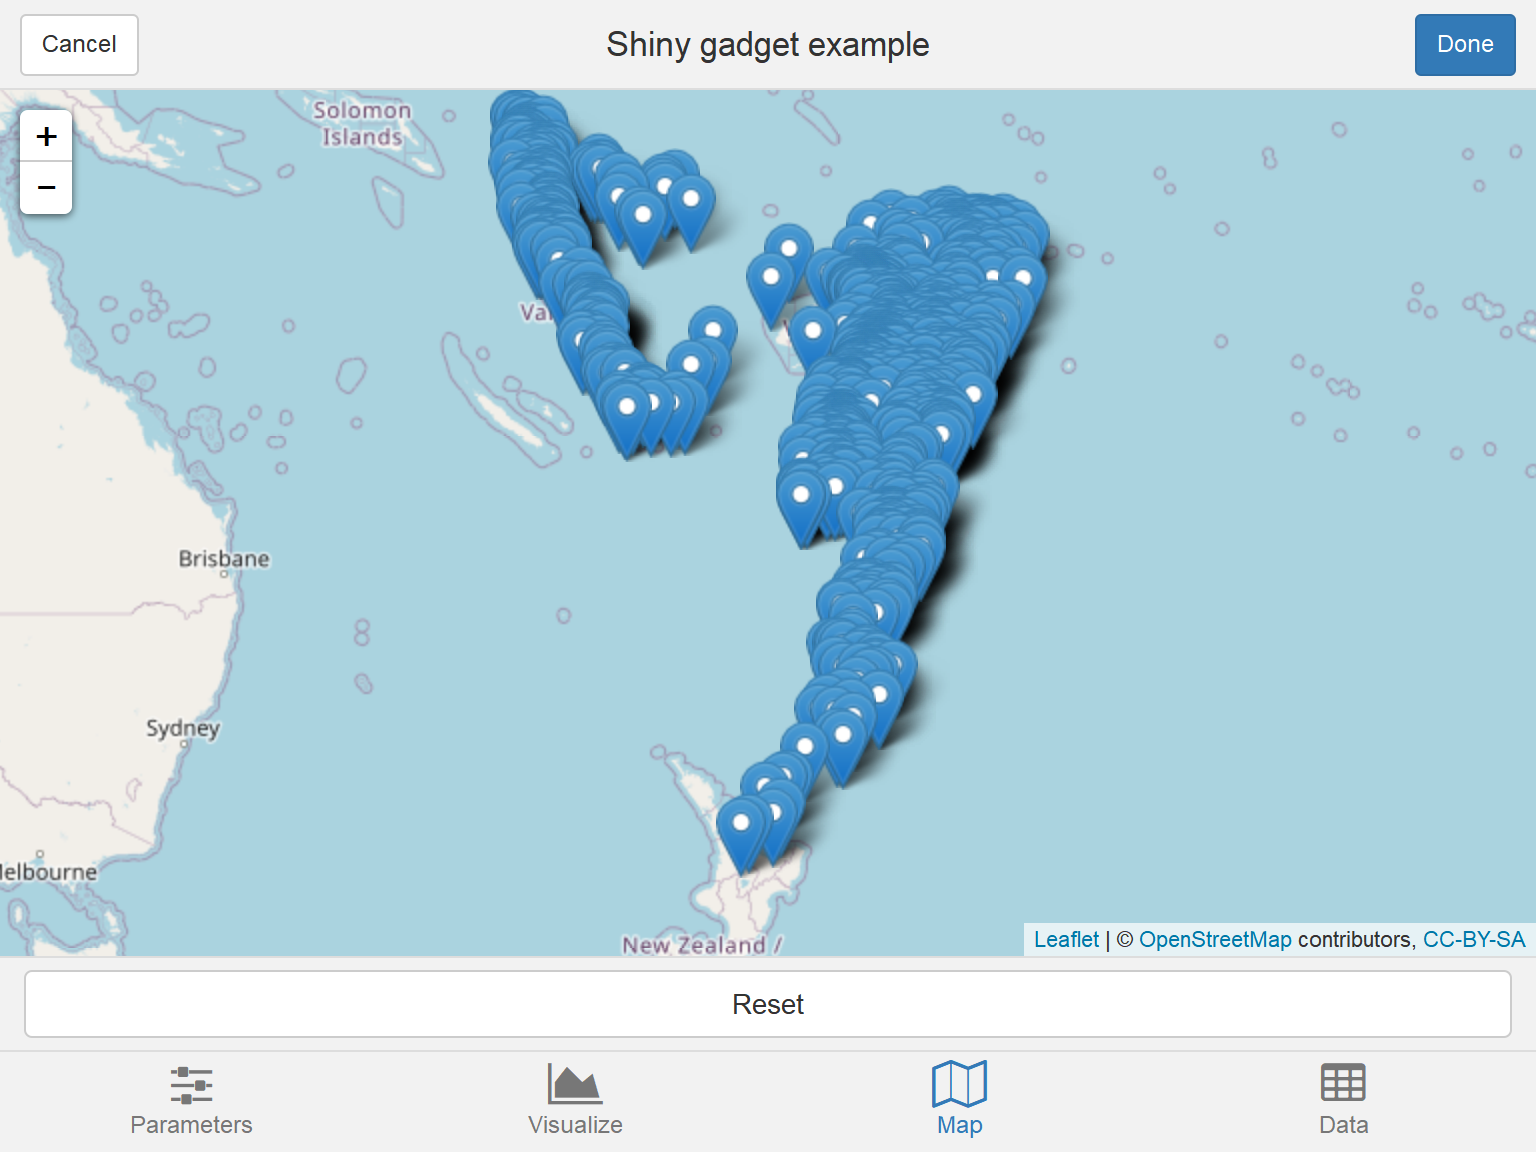
\includegraphics{bookdown-book-zhCN_files/figure-latex/miniUI-1} }

}

\caption{通过 miniUI 软件包创建的一个 Shiny 应用;你可以在 <https://yihui.shinyapps.io/miniUI/> 看到在线版本}\label{fig:miniUI}
\end{figure}

\let\href\ooldhref

同样的,如果你正在阅读本书的 HTML 版本,将看到一个活动的应用程序,如果你正在阅读本书的其他格式版本,将看到一个静态屏幕截图。上面的 Shiny 应用程序是使用 \textbf{miniUI} 软件包 \citep{R-miniUI} 创建的,这个软件包提供的布局功能对于小屏幕上的 Shiny 应用程序特别好。如果使用普通的 Shiny 布局功能,则可能会在 iframe 中看到垂直和/或水平滚动条,因为页面大小太大,无法放入 iframe 中。如果 iframe 的默认宽度太小,可以使用区块选项 \texttt{out.width} 进行更改。对于 iframe 的高度,请使用 \texttt{include\_url()}/\texttt{include\_app()} 的 \texttt{height} 参数。

Shiny 应用程序可能需要比普通 URL 更长的加载时间。你可能需要对 \texttt{delay} 选项使用一个保守的值,例如 10。不用多加叙说,\texttt{include\_url()} 和 \texttt{include\_app()} 需要一个正常工作的 Internet 连接,除非你以前缓存了区块(但是如果没有 Internet 连接,iframe 内的网页仍然无法工作)。

\chapter{输出格式}\label{output-formats}

\textbf{bookdown} 软件包主要支持三种类型的输出格式:HTML、LaTeX/PDF 和电子书。在本章中,我们将介绍这些格式的可能的配置项。输出格式可以在书籍的第一个 Rmd 文件中的 YAML 元数据中指定,也可以在书籍根目录下名为 \texttt{\_output.yml} 的单独 YAML 文件中指定。以下是前者的简要示例(输出格式在 YAML 元数据中的 \texttt{output} 字段中指定):

\begin{Shaded}
\begin{Highlighting}[]
\PreprocessorTok{{-}{-}{-}}
\FunctionTok{title}\KeywordTok{:}\AttributeTok{ }\StringTok{"一本令人印象深刻的书"}
\FunctionTok{author}\KeywordTok{:}\AttributeTok{ }\StringTok{"李雷和韩梅梅"}
\FunctionTok{output}\KeywordTok{:}
\AttributeTok{  bookdown:}\FunctionTok{:gitbook}\KeywordTok{:}
\AttributeTok{    }\FunctionTok{lib\_dir}\KeywordTok{:}\AttributeTok{ assets}
\AttributeTok{    }\FunctionTok{split\_by}\KeywordTok{:}\AttributeTok{ section}
\AttributeTok{    }\FunctionTok{config}\KeywordTok{:}
\AttributeTok{      }\FunctionTok{toolbar}\KeywordTok{:}
\AttributeTok{        }\FunctionTok{position}\KeywordTok{:}\AttributeTok{ static}
\AttributeTok{  bookdown:}\FunctionTok{:pdf\_book}\KeywordTok{:}
\AttributeTok{    }\FunctionTok{keep\_tex}\KeywordTok{:}\AttributeTok{ }\CharTok{true}
\AttributeTok{  bookdown:}\FunctionTok{:html\_book}\KeywordTok{:}
\AttributeTok{    }\FunctionTok{css}\KeywordTok{:}\AttributeTok{ toc.css}
\FunctionTok{documentclass}\KeywordTok{:}\AttributeTok{ book}
\PreprocessorTok{{-}{-}{-}}
\end{Highlighting}
\end{Shaded}

这是 \texttt{\_output.yml}\index{\_output.yml} 的示例:

\begin{Shaded}
\begin{Highlighting}[]
\AttributeTok{bookdown:}\FunctionTok{:gitbook}\KeywordTok{:}
\AttributeTok{  }\FunctionTok{lib\_dir}\KeywordTok{:}\AttributeTok{ assets}
\AttributeTok{  }\FunctionTok{split\_by}\KeywordTok{:}\AttributeTok{ section}
\AttributeTok{  }\FunctionTok{config}\KeywordTok{:}
\AttributeTok{    }\FunctionTok{toolbar}\KeywordTok{:}
\AttributeTok{      }\FunctionTok{position}\KeywordTok{:}\AttributeTok{ static}
\AttributeTok{bookdown:}\FunctionTok{:pdf\_book}\KeywordTok{:}
\AttributeTok{  }\FunctionTok{keep\_tex}\KeywordTok{:}\AttributeTok{ }\CharTok{true}
\AttributeTok{bookdown:}\FunctionTok{:html\_book}\KeywordTok{:}
\AttributeTok{  }\FunctionTok{css}\KeywordTok{:}\AttributeTok{ toc.css}
\end{Highlighting}
\end{Shaded}

在这种情况下,所有格式配置都应该在顶层,而不是在 \texttt{output} 字段下。在 \texttt{\_output.yml} 文件中你不需要这三个破折号 \texttt{-\/-\/-}。

\section{HTML}\label{html}

编译一本书(使用 \textbf{bookdown})与编译一个单独的 R Markdown 文档(使用 \textbf{rmarkdown})为 HTML\index{HTML} 格式的主要区别在于,默认情况下一本书籍会生成多个 HTML 页面------通常每章一个 HTML 文件。这使得你在阅读书籍某一章节的时候能够更容易地添加书签或将其 URL 分享给他人,并且可以更快地将书籍加载到 Web 浏览器中。目前,我们为 HTML 输出提供了多种不同地样式:

\begin{itemize}
\tightlist
\item
  GitBook 样式 (Section \ref{gitbook-style}),
\item
  三列 Bootstrap 样式 (Section \ref{bs4-book}),
\item
  默认的 Bootstrap 样式 (Section \ref{bootstrap-style})
\item
  Tufte 样式 (Section \ref{tufte-style}).
\end{itemize}

\subsection{GitBook 样式}\label{gitbook-style}

GitBook 样式来自于 GitBook\index{GitBook},这是一个由 Friendcode, Inc 公司发起的项目 (\url{https://www.gitbook.com}),它致力于帮助作者使用 Markdown 撰写书籍。它提供了一种漂亮的风格,其布局由左侧显示目录的侧边栏和右侧的书籍主题组成。该设计能够对窗口大小变化做出响应,例如,当窗口足够宽时,导航按钮显示在书籍主体的左侧/右侧,当窗口较窄时,导航按钮折叠到底部,一边给读者更多的水平空间来阅读书籍主体部分。

开始撰写一本新的 \texttt{gitbook} 的最简单的方法就是使用 RStudio Project Wizard(\emph{文件 (File) \textgreater{} 新建项目 (New Project) \textgreater{} 新的目录 (New Directory) \textgreater{} 使用 bookdown 的书籍项目 (Book project using bookdown)})并在下拉菜单中选择 \texttt{gitbook}(见图 \ref{fig:new-bs4-book})。

如果你不使用 RStudio 或更喜欢使用函数,则可以从 R console 中使用 \texttt{bookdown::create\_gitbook()} 创建相同的项目模板。请参阅 \texttt{?bookdown::create\_gitbook} 以获取帮助。

我们对原始的 GitBook 项目做了一些改进。最重要的一点是,我们将 Markdown 引擎替换为基于 Pandoc 的 R Markdown v2,这样你在写书时可以使用更多的功能:

\begin{itemize}
\tightlist
\item
  你可以在 Markdown 中嵌入 R 代码块和内联 R 表达式,这样可以轻松创建可重复的 (reproducible) 文档,并使你不必手动同步计算过程与它的实际输出结果(\textbf{knitr} 将自动处理)。
\item
  Markdown 语法更加丰富:你可以编写 Pandoc 版本的 Markdown 支持的任何内容,例如 LaTeX 数学表达式和引文。
\item
  你可以在书中嵌入交互式内容(仅用于 HTML 输出)。例如 HTML 小组件和 Shiny 应用程序。
\end{itemize}

我们还在用户界面中添加了一些有用的特性,很快我们将详细介绍它们。\textbf{bookdown} 中 GitBook 样式的输出格式函数为 \texttt{gitbook()}。它的参数如下所示:

\begin{Shaded}
\begin{Highlighting}[]
\FunctionTok{gitbook}\NormalTok{(}\AttributeTok{fig\_caption =} \ConstantTok{TRUE}\NormalTok{, }\AttributeTok{number\_sections =} \ConstantTok{TRUE}\NormalTok{,}
  \AttributeTok{self\_contained =} \ConstantTok{FALSE}\NormalTok{, }\AttributeTok{anchor\_sections =} \ConstantTok{TRUE}\NormalTok{,}
  \AttributeTok{lib\_dir =} \StringTok{"libs"}\NormalTok{,}
  \AttributeTok{global\_numbering =} \SpecialCharTok{!}\NormalTok{number\_sections,}
  \AttributeTok{pandoc\_args =} \ConstantTok{NULL}\NormalTok{, }\AttributeTok{extra\_dependencies =} \FunctionTok{list}\NormalTok{(), ...,}
  \AttributeTok{template =} \StringTok{"default"}\NormalTok{,}
  \AttributeTok{split\_by =} \FunctionTok{c}\NormalTok{(}\StringTok{"chapter"}\NormalTok{, }\StringTok{"chapter+number"}\NormalTok{, }\StringTok{"section"}\NormalTok{, }\StringTok{"section+number"}\NormalTok{, }\StringTok{"rmd"}\NormalTok{, }\StringTok{"none"}\NormalTok{),}
  \AttributeTok{split\_bib =} \ConstantTok{TRUE}\NormalTok{, }\AttributeTok{config =} \FunctionTok{list}\NormalTok{(), }\AttributeTok{table\_css =} \ConstantTok{TRUE}\NormalTok{,}
  \AttributeTok{code\_folding =} \FunctionTok{c}\NormalTok{(}\StringTok{"none"}\NormalTok{, }\StringTok{"show"}\NormalTok{, }\StringTok{"hide"}\NormalTok{))}
\end{Highlighting}
\end{Shaded}

大多数参数被传递给 \texttt{rmarkdown::html\_document()},包括 \texttt{fig\_caption}、\texttt{lib\_dir} 和 \texttt{...}。想要了解所有可能参数的完整列表,你可以查阅 \texttt{rmarkdown::html\_document()} 的帮助页面。我们强烈推荐你使用 \texttt{fig\_caption\ =\ TRUE},原因由两个:1) 使用标题来解释你的图片很重要;2) 启用图片标题意味着当输出为 LaTeX 时,图片将被放置在浮动环境中,否则可能会在某些页面上留下大量空白。图/表编号的格式取决于章节是否编号:如果 \texttt{number\_sections\ =\ TRUE},这些编号数字会使用 \texttt{X.i} 的格式,其中 \texttt{X} 是篇章编号而 \texttt{i} 是递增编号;如果章节没有编号,所有的图/表在书籍中将从 1、2、\ldots\ldots、N 开始依次编号。请注意,在任何一种情况下,图片和表格的编号都是相互独立的。

在 \texttt{...} 的所有可能的参数之中,你最可能使用参数 \texttt{css} 提供一个或多个自定义的 CSS 文件来调整默认 CSS 样式。在 \texttt{gitbook()} 中有一些 \texttt{html\_document()} 的参数被硬编码,你无法更改它们:\texttt{toc\ =\ TRUE}(必须使用目录)、\texttt{theme\ =\ NULL}(不使用任何 Bootstrap 主题)和 \texttt{template}(存在一个内部 GitBook 模板)。

请注意,如果将参数修改为 \texttt{self\_contained\ =\ TRUE} 以更改 HTML 页面为自包含的 HTML 页面,则所有 HTML 文件的总大小都会显著增加,因为每个 HTML 文件中都必须嵌入许多 JS 和 CSS 文件。

除了这些 \texttt{html\_document()} 的配置项之外,\texttt{gitbook()} 还有另外三个参数:\texttt{split\_by}、\texttt{split\_bib} 和 \texttt{config}。参数 \texttt{split\_by} 指定了如何将 HTML 输出文件拆分为多个页面,其可能的值为:

\begin{itemize}
\tightlist
\item
  \texttt{rmd}:使用输入的 Rmd 文件的文件名作为对应 HTML 文件的文件名,例如,\texttt{chapter3.Rmd} 生成的 HTML 文件为 \texttt{chapter3.html}。
\item
  \texttt{none}:不要拆分 HTML 文件(整本书将是一个 HTML 文件)。
\item
  \texttt{chapter}:按一级标题拆分文件。
\item
  \texttt{section}:按二级标题拆分文件。
\item
  \texttt{chapter+number} 和 \texttt{section+number}: 与 \texttt{chapter} 和 \texttt{section} 类似,但是文件将被编号。
\end{itemize}

对于 \texttt{chapter} 和 \texttt{section},HTML 文件名将由标题标识符确定,例如,篇章标题为 \texttt{\#\ Introduction} 的第一章的文件名默认为 \texttt{introduction.html}。对于 \texttt{chapter+number} 和 \texttt{section+number},章/节编号将在 HTML 文件名之前,例如 \texttt{1-introduction.html} 和 \texttt{2-1-literature.html}。默认情况下,标题标识符是从标题文本自动生成的,\footnote{要查看有关如何自动生成标识符的更多详细内容,请参阅 Pandoc 文档中 \texttt{auto\_identifiers} 扩展相关内容 \url{http://pandoc.org/MANUAL.html\#header-identifiers}}你页可以在标题文本后使用语法 \texttt{\{your-custom-id\}} 手动指定标识符,例如:

\begin{Shaded}
\begin{Highlighting}[]
\FunctionTok{\# An Introduction \{\#introduction\}}

\NormalTok{默认标识符是 }\InformationTok{\textasciigrave{}an{-}introduction\textasciigrave{}}\NormalTok{,}
\NormalTok{但是我们将其更改为 }\InformationTok{\textasciigrave{}introduction\textasciigrave{}}\NormalTok{。}
\end{Highlighting}
\end{Shaded}

默认情况下,参考书目会被拆分,相关的引文项目将放在每页的底部,这样读者就不必导航到不同的参考书目页面来查看引文的详细信息。可以使用 \texttt{split\_bib\ =\ FALSE} 禁用此功能,在这种情况下,所有引文都放在单独的页面上。

你可以使用 \texttt{config} 配置项中的几个子配置项来调整用户界面中的一些细节。回想一下,所有输出格式配置项(不仅仅适用于 \texttt{bookdown::gitbook})都可以通过使用命令行接口 \texttt{bookdown::render\_book()} 传递给格式函数,或直接将其写入 YAML 元数据。我们将 \texttt{gitbook} 格式下 \texttt{config} 的默认子配置项显示为 YAML 元数据并展示如下(请注意,它们的缩进都在 \texttt{config} 配置项下):

\begin{Shaded}
\begin{Highlighting}[]
\AttributeTok{bookdown:}\FunctionTok{:gitbook}\KeywordTok{:}
\AttributeTok{  }\FunctionTok{config}\KeywordTok{:}
\AttributeTok{    }\FunctionTok{toc}\KeywordTok{:}
\AttributeTok{      }\FunctionTok{collapse}\KeywordTok{:}\AttributeTok{ subsection}
\AttributeTok{      }\FunctionTok{scroll\_highlight}\KeywordTok{:}\AttributeTok{ }\CharTok{true}
\AttributeTok{      }\FunctionTok{before}\KeywordTok{:}\AttributeTok{ }\CharTok{null}
\AttributeTok{      }\FunctionTok{after}\KeywordTok{:}\AttributeTok{ }\CharTok{null}
\AttributeTok{    }\FunctionTok{toolbar}\KeywordTok{:}
\AttributeTok{      }\FunctionTok{position}\KeywordTok{:}\AttributeTok{ fixed}
\AttributeTok{    }\FunctionTok{edit }\KeywordTok{:}\AttributeTok{ }\CharTok{null}
\AttributeTok{    }\FunctionTok{download}\KeywordTok{:}\AttributeTok{ }\CharTok{null}
\AttributeTok{    }\FunctionTok{search}\KeywordTok{:}
\AttributeTok{      }\FunctionTok{engine}\KeywordTok{:}\AttributeTok{ lunr}\CommentTok{ \# or fuse}
\CommentTok{      \# options to control/tune search engine behavior (for}
\CommentTok{      \# fuse.js, refer to https://fusejs.io/api/options.html)}
\AttributeTok{      }\FunctionTok{options}\KeywordTok{:}\AttributeTok{ }\CharTok{null}
\AttributeTok{    }\FunctionTok{fontsettings}\KeywordTok{:}
\AttributeTok{      }\FunctionTok{theme}\KeywordTok{:}\AttributeTok{ white}
\AttributeTok{      }\FunctionTok{family}\KeywordTok{:}\AttributeTok{ sans}
\AttributeTok{      }\FunctionTok{size}\KeywordTok{:}\AttributeTok{ }\DecValTok{2}
\AttributeTok{    }\FunctionTok{sharing}\KeywordTok{:}
\AttributeTok{      }\FunctionTok{facebook}\KeywordTok{:}\AttributeTok{ }\CharTok{true}
\AttributeTok{      }\FunctionTok{github}\KeywordTok{:}\AttributeTok{ }\CharTok{false}
\AttributeTok{      }\FunctionTok{twitter}\KeywordTok{:}\AttributeTok{ }\CharTok{true}
\AttributeTok{      }\FunctionTok{linkedin}\KeywordTok{:}\AttributeTok{ }\CharTok{false}
\AttributeTok{      }\FunctionTok{weibo}\KeywordTok{:}\AttributeTok{ }\CharTok{false}
\AttributeTok{      }\FunctionTok{instapaper}\KeywordTok{:}\AttributeTok{ }\CharTok{false}
\AttributeTok{      }\FunctionTok{vk}\KeywordTok{:}\AttributeTok{ }\CharTok{false}
\AttributeTok{      }\FunctionTok{whatsapp}\KeywordTok{:}\AttributeTok{ }\CharTok{false}
\AttributeTok{      }\FunctionTok{all}\KeywordTok{:}\AttributeTok{ }\KeywordTok{[}\StringTok{\textquotesingle{}facebook\textquotesingle{}}\KeywordTok{,}\AttributeTok{ }\StringTok{\textquotesingle{}twitter\textquotesingle{}}\KeywordTok{,}\AttributeTok{ }\StringTok{\textquotesingle{}linkedin\textquotesingle{}}\KeywordTok{,}\AttributeTok{ }\StringTok{\textquotesingle{}weibo\textquotesingle{}}\KeywordTok{,}\AttributeTok{ }\StringTok{\textquotesingle{}instapaper\textquotesingle{}}\KeywordTok{]}
\AttributeTok{    }\FunctionTok{info}\KeywordTok{:}\AttributeTok{ }\CharTok{true}
\end{Highlighting}
\end{Shaded}

\texttt{toc} 配置项控制目录 (TOC) 的行为。当加载页面时,你可以通过 \texttt{collapse} 配置项先将某些项目折叠。该配置项可能的值为 \texttt{subsection}、\texttt{section}、\texttt{none}(或 \texttt{null})。如果你的目录很长且标题超过三个级别,则这个配置项可能会有所帮助:\texttt{subsection} 表示折叠目录项目中的所有小节 (X.X.X);\texttt{section} 表示折叠目录项目中的所有节 (X.X),因此最初仅显示顶级标题;\texttt{none} 表示不折叠目录中的任何项目。对于那些折叠的目录项目,可以通过单击其上级目录项目来切换其可见性。例如,你可以单击目录中的篇章标题以显示/隐藏该章的小节。

\texttt{toc} 中的 \texttt{scroll\_highlight} 配置项控制在滚动书籍正文页面时是否启用目录项目的高亮显示(默认情况下此功能已启用)。当向下/向上滚动时,每当新标题进入当前视口,左侧目录中的相应项目将高亮显示。

由于侧边栏的宽度是固定的,因此当目录中的某个项目由于标题文本太宽而被截断时,可以将光标悬停在侧边栏上以查看显示全部文字的提示条。

你可以使用 HTML 标签 \texttt{\textless{}li\textgreater{}} 在目录前后添加更多项目。这些项目将使用水平分隔器与目录分开。你可以使用管道符 \texttt{\textbar{}},这样就不需要按照 YAML 语法转义这些项目中的任何字符,例如:

\begin{verbatim}
    toc:
      before: |
        <li><a href="...">My Awesome Book</a></li>
        <li><a href="...">John Smith</a></li>
      after: |
        <li><a href="https://github.com/rstudio/bookdown">
        Proudly published with bookdown</a></li>
\end{verbatim}

当你浏览不同的 HTML 页面时,我们将尝试保留目录的滚动位置。通常即使你转到下一页,也会在目录的固定位置上看到滚动条。但是如果当前章/节的目录项目在页面加载时不可见,我们将自动滚动目录以使其对你可见。

\begin{figure}

\includegraphics[width=1\linewidth]{images/gitbook} \caption{The GitBook toolbar.}\label{fig:gitbook-toolbar}
\end{figure}

Gitbook 样式在每个页面的顶部都有一个工具栏(图 \ref{fig:gitbook-toolbar}),允许你动态地改变书籍设置。\texttt{toolbar} 配置项有一个子配置项 \texttt{position},可以取值为 \texttt{fixed} 或 \texttt{static}。默认情况下 (\texttt{fixed}),工具栏将被固定在页面的顶部,所以即使你向下滚动页面,工具栏也仍然在顶部可见。如果它被设置为 \texttt{static},工具栏将不会随着页面滚动,也就是说,一旦滚动页面,你将无法看到它。

工具栏的第一个按钮可以切换侧边栏的可见性。你也可以敲击键盘上的 \texttt{S} 键来做同样的事。GitBook 样式能够记住侧边栏的可见性状态,例如,如果你关闭了侧边栏,那么下次打开书籍时,侧边栏将保持隐藏状态。事实上,GitBook 样式也能够记住许多其它的设置,例如搜索关键词和字体设置。

工具栏的第二个按钮是搜索按钮。它的键盘快捷键是 \texttt{F}(查找)。点击该按钮后,你会看到侧边栏的顶部出现一个搜索框。当你在框中输入时,目录项将会被过滤,以显示符合搜索关键词的部分。现在你可以使用方向键 \texttt{Up}/\texttt{Down} 来突出显示搜索结果中的上一个或下一个匹配内容。当你再次点击搜索按钮(或在搜索框外敲击 \texttt{F}),搜索关键词将被清空,搜索框将被隐藏。如果要禁用搜索,请在 \texttt{config} 中设置 \texttt{search:\ false} 配置项。

第三个按钮是用于字体/主题设置。读者可以改变字体大小(更大或更小),字体族(有衬线 (serif) 或无衬线 (sans serif)),以及主题(\texttt{White}、\texttt{Sepia} 或 \texttt{Nignt})。你可以通过 \texttt{fontsettings} 配置项设置这些配置项的初始值。字体大小是按 0-4 的比例测量的;初始值可以设置为 1、2(默认)、3 或 4。可以通过设置 \texttt{fontsettings:\ null}(或 \texttt{no})将该按钮从工具栏中删除。

\begin{Shaded}
\begin{Highlighting}[]
\CommentTok{\# changing the default}
\AttributeTok{    }\FunctionTok{fontsettings}\KeywordTok{:}
\AttributeTok{      }\FunctionTok{theme}\KeywordTok{:}\AttributeTok{ night}
\AttributeTok{      }\FunctionTok{family}\KeywordTok{:}\AttributeTok{ serif}
\AttributeTok{      }\FunctionTok{size}\KeywordTok{:}\AttributeTok{ }\DecValTok{3}
\end{Highlighting}
\end{Shaded}

\texttt{edit}(编辑)配置项与第 \ref{configuration} 节中提到的配置项相同。如果它不为空,一个编辑按钮将被添加到工具栏中。这是为书籍的潜在贡献者设计的,他们可以在点击该按钮后在 GitHub 上编辑书籍内容并发送 Pull Requests。\texttt{history} 和 \texttt{View} 配置项的工作方式也是如此。

如果你的书有其它输出格式供读者下载,你可以提供 \texttt{download} 选项,这样就可以在工具栏中添加一个下载按钮。这个配置项可以接受一个字符向量,或者一个字符向量的列表,其中每个向量的长度为 2。当它是一个字符向量时,它应该包含文件名或文件扩展名,例如,以下两种设置都是正确的。

\begin{Shaded}
\begin{Highlighting}[]
\AttributeTok{    }\FunctionTok{download}\KeywordTok{:}\AttributeTok{ }\KeywordTok{[}\StringTok{"book.pdf"}\KeywordTok{,}\AttributeTok{ }\StringTok{"book.epub"}\KeywordTok{]}
\AttributeTok{    }\FunctionTok{download}\KeywordTok{:}\AttributeTok{ }\KeywordTok{[}\StringTok{"pdf"}\KeywordTok{,}\AttributeTok{ }\StringTok{"epub"}\KeywordTok{,}\AttributeTok{ }\StringTok{"mobi"}\KeywordTok{]}
\end{Highlighting}
\end{Shaded}

当你只提供文件扩展名时,文件名来自于配置文件 \texttt{\_bookdown.yml}(第 \ref{configuration} 节)中的书籍文件名。当 \texttt{download} 为 \texttt{null} 时,\texttt{gitbook()} 将在书籍输出目录中寻找 PDF、EPUB 和 MOBI 文件,并自动将它们加入 \texttt{download} 配置项中。如果你只是想关闭下载按钮,请使用 \texttt{download:\ false}。所有供读者下载的文件将显示在一个下拉菜单中,文件扩展名被用作菜单文本。当唯一可供读者下载的格式是 PDF 时,下载按钮将是一个单一的 PDF 按钮而不是一个下拉菜单。

 \&esmp;另一种形式的 \texttt{download} 配置项的值是一个长度为 2 的向量构成的列表,例如:

\begin{Shaded}
\begin{Highlighting}[]
\AttributeTok{    }\FunctionTok{download}\KeywordTok{:}\AttributeTok{ }\KeywordTok{[[}\StringTok{"book.pdf"}\KeywordTok{,}\AttributeTok{ }\StringTok{"PDF"}\KeywordTok{],}\AttributeTok{ }\KeywordTok{[}\StringTok{"book.epub"}\KeywordTok{,}\AttributeTok{ }\StringTok{"EPUB"}\KeywordTok{]]}
\end{Highlighting}
\end{Shaded}

你也可以把它写成这样:

\begin{Shaded}
\begin{Highlighting}[]
\AttributeTok{    }\FunctionTok{download}\KeywordTok{:}
\AttributeTok{      }\KeywordTok{{-}}\AttributeTok{ }\KeywordTok{[}\StringTok{"book.pdf"}\KeywordTok{,}\AttributeTok{ }\StringTok{"PDF"}\KeywordTok{]}
\AttributeTok{      }\KeywordTok{{-}}\AttributeTok{ }\KeywordTok{[}\StringTok{"book.epub"}\KeywordTok{,}\AttributeTok{ }\StringTok{"EPUB"}\KeywordTok{]}
\end{Highlighting}
\end{Shaded}

列表中的每个向量由文件名和将在菜单中显示的文本组成。与第一种形式相比,这种形式允许你自定义菜单文本,例如,你可能有两份不同的 PDF 供读者下载,因此需要使菜单项目有所差别。

在工具栏的右边有一些按钮,它们可以让你在社会网络网站,如 Twitter、Facebook 和 Linkedin 上分享链接。你可以使用 \texttt{sharing} 配置项来决定启用哪些按钮。如果你想完全摆脱这些按钮,可以使用 \texttt{sharing:\ null}(或 \texttt{no})。

工具栏中显示的另一个按钮是信息 (\texttt{i}) 按钮,它列出了可用于导航文档的键盘快捷方式。这个按钮可以通过设置 \texttt{info:\ false} 来隐藏。

最后,YAML 元数据中还有一些顶级配置项,可以通过 Pandoc 传递给 GitBook HTML 模板。它们可能不会对 HTML 输出产生明显的影响,但当你把 HTML 输出部署为网站时,它们可能会很有用。这些选项包括:

\begin{itemize}
\tightlist
\item
  \texttt{description}: 一个字符串,它将会被写入 HTML 头部 \texttt{\textless{}meta\ name="description"\ content=""\textgreater{}} 标签中的 \texttt{content} 属性(如果缺失,将会使用书籍的标题替代)。这对搜索引擎优化 (search engine optimization, SEO) 很有用。请注意,它应该是纯文本,不应该使用任何 Markdown 格式,例如 \texttt{\_italic\_} 或 \texttt{**bold**}。
\item
  \texttt{url}: 书籍网站的 URL,例如 \texttt{https\textbackslash{}://bookdown.org/yihui/bookdown/}。\footnote{在 \texttt{:} 之前插入的反斜杠是因为一个技术问题:我们要防止 Pandoc 将链接翻译为 HTML 代码 \texttt{\textless{}a\ href="..."\textgreater{}\textless{}/a\textgreater{}}。在 \url{https://github.com/jgm/pandoc/issues/2139} 上你能够看到更多细节}
\item
  \texttt{github-repo}: \texttt{user/repo} 格式的 GitHub 储存库。
\item
  \texttt{cover-image}: 书籍封面图片文件的路径。
\item
  \texttt{apple-touch-icon}: 一个图标文件的路径(例如一个 PNG 图片)。这只适用于 iOS 系统:当网站被添加到主屏幕上时,该链接由这个图标表示。
\item
  \texttt{apple-touch-icon-size}: 图标文件的大小(默认情况下为 152 x 152 像素)。
\item
  \texttt{favicon}: \texttt{favorite\ icon}(收藏夹图标)文件的路径。通常情况下,这个图标显示在浏览器的地址栏中,如果浏览器支持标签,则显示在标签的页面标题前方。
\end{itemize}

下面我们展示了一下 YAML 元数据的样例(请再次注意这些是 \emph{顶级} 配置项):

\begin{Shaded}
\begin{Highlighting}[]
\PreprocessorTok{{-}{-}{-}}
\FunctionTok{title}\KeywordTok{:}\AttributeTok{ }\StringTok{"An Awesome Book"}
\FunctionTok{author}\KeywordTok{:}\AttributeTok{ }\StringTok{"John Smith"}
\FunctionTok{description}\KeywordTok{:}\AttributeTok{ }\StringTok{"This book introduces the ABC theory, and ..."}
\FunctionTok{url}\KeywordTok{:}\AttributeTok{ }\StringTok{\textquotesingle{}https\textbackslash{}://bookdown.org/john/awesome/\textquotesingle{}}
\FunctionTok{github{-}repo}\KeywordTok{:}\AttributeTok{ }\StringTok{"john/awesome"}
\FunctionTok{cover{-}image}\KeywordTok{:}\AttributeTok{ }\StringTok{"images/cover.png"}
\FunctionTok{apple{-}touch{-}icon}\KeywordTok{:}\AttributeTok{ }\StringTok{"touch{-}icon.png"}
\FunctionTok{apple{-}touch{-}icon{-}size}\KeywordTok{:}\AttributeTok{ }\DecValTok{120}
\FunctionTok{favicon}\KeywordTok{:}\AttributeTok{ }\StringTok{"favicon.ico"}
\PreprocessorTok{{-}{-}{-}}
\end{Highlighting}
\end{Shaded}

设置 \texttt{description} 和 \texttt{cover-image} 的一个很好的效果是,当你在一些社交网站(如 Twitter)上分享你的书籍的链接时,该链接可以自动扩展为一个带有封面图片和书籍描述的卡片。

\subsection{三列 Bootstrap 样式}\label{bs4-book}

\texttt{bs4\_book()} 输出格式是使用 Bootstrap (\url{https://getbootstrap.com}) 构建的,其功能经过了精心设计,无论你是在手机、平板电脑还是桌面上,都能获得干净的阅读体验。在全尺寸屏幕上,其布局包括散列内容,因此读者能够快速看到左边的所有章节,中间的当前章节,右边的当前篇章中的各个小节。你可以在这里阅读样例书籍:\url{https://mastering-shiny.org}

\begin{figure}

{\centering \href{https://mastering-shiny.org}{
\includegraphics{images/bs4-book} }

}

\caption{Home page of a book with the three-column Bootstrap style.}\label{fig:unnamed-chunk-12}
\end{figure}

除了基础的 \textbf{bookdown} 组件(第 \ref{components} 节),\texttt{bs4\_book} 的主要功能包括:

\begin{itemize}
\item
  使用 \href{https://pkgs.rstudio.com/bslib/}{\textbf{bslib} 软件包}轻松定制颜色和字体。
\item
  内置搜索(按小节细分),帮助读者快速查找所需内容。
\item
  包含章节内目录的侧边栏,使得书籍导航更加简单,有助于提供在本章中有关当前位置的上下文。
\item
  精心排版,不管设备的大小,都尽可能使得内容易于阅读。在阅读时,一个悬浮标题会妨碍你的阅读,但是如果你需要的话,它很容易被访问。
\item
  行内脚注意味着你能够在它们所指文本的旁边阅读旁白。此主题最好与生成脚注的参考样式匹配。
\item
  通过 \href{https://downlit.r-lib.org}{\textbf{downlit} 软件包}进行的 R 语法高亮和自动链接,并搭配 Alison Hill 设计的无障碍配色方案。
\item
  增强了通过 Twitter、LinkedIn 和 Facebook等平台进行社会分享的元数据,这样,每一个分享的章节都会有一个独特的描述,根据该章节的内容自动生成。
\item
  配置指向远程存储库(如 GitHub 或 GitLab)的链接的能力,允许读者轻松查看每个章节的源文件或提供编辑建议。
\end{itemize}

输出格式函数是 \href{https://pkgs.rstudio.com/bookdown/reference/bs4_book.html}{\texttt{bookdown::bs4\_book}}。以下是它的参数:

\begin{Shaded}
\begin{Highlighting}[]
\FunctionTok{bs4\_book}\NormalTok{(}\AttributeTok{theme =} \FunctionTok{bs4\_book\_theme}\NormalTok{(), }\AttributeTok{repo =} \ConstantTok{NULL}\NormalTok{, ...,}
  \AttributeTok{lib\_dir =} \StringTok{"libs"}\NormalTok{, }\AttributeTok{pandoc\_args =} \ConstantTok{NULL}\NormalTok{,}
  \AttributeTok{extra\_dependencies =} \ConstantTok{NULL}\NormalTok{, }\AttributeTok{template =} \StringTok{"default"}\NormalTok{,}
  \AttributeTok{split\_bib =} \ConstantTok{FALSE}\NormalTok{, }\AttributeTok{footnotes\_inline =} \ConstantTok{TRUE}\NormalTok{)}
\end{Highlighting}
\end{Shaded}

\subsubsection{\texorpdfstring{创作一本 \texttt{bs4\_book}}{创作一本 bs4\_book}}\label{ux521bux4f5cux4e00ux672c-bs4_book}

开始撰写一本新的 \texttt{bs4\_book} 的最简单的方法就是使用 RStudio 项目向导 (Project Wizard)(\emph{File(文件) \textgreater{} New Project(新的项目) \textgreater{} New Directory(新的目录) \textgreater{} Book project using bookdown(使用 bookdown 的书籍项目)}) 并在下拉菜单中选择 \texttt{bs4\_book}。(请见图 \ref{fig:new-bs4-book})。

\begin{figure}

{\centering 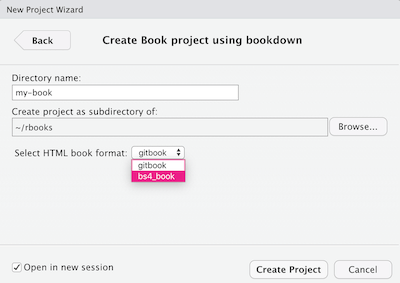
\includegraphics{images/new-bs4-book} 

}

\caption{用于创建新的 bookdown 项目的 RStudio 项目向导的屏幕截图。}\label{fig:new-bs4-book}
\end{figure}

如果你不使用 RStudio 或者喜欢使用函数来完成,可以在 R Console 中使用 \texttt{bookdown::create\_bs4\_book()} 创建相同的项目模板。参见 \texttt{?bookdown::create\_bs4\_book}或\href{https://pkgs.rstudio.com/bookdown/reference/create_book.html}{在线文档}以获得帮助。

这种风格是为每页展示一个章节的书籍设计的。这意味着每章是一个 \texttt{.Rmd} 文件,每个 \texttt{.Rmd} 文件可以包含一个章节。每个文件\emph{必须}以一级标题开始,例如 \texttt{\#\ 章节标题},而且必须是文件中唯一的一级标题。

在章节中使用第二级和更低级的标题,如:

\begin{Shaded}
\begin{Highlighting}[]
\FunctionTok{\#   一章}

\FunctionTok{\#\#  一节}

\FunctionTok{\#\#\# 一小节}
\end{Highlighting}
\end{Shaded}

第一级和第二级标题显示在当前章节的侧边栏中,当你向下滚动时,它会粘在页面顶部。当导航到一节时,像 \texttt{小节} 这样的三级子标题将自动展开。

\texttt{index.Rmd} 文件是必需的,并且也是你的书籍的第一章。当你编译书籍时,它将会成为主页面。如果你想将仅应包含在书籍 HTML 版本的内容包括在内,你可能需要将 \textbf{knitr} \texttt{include} 区块配置项与 \texttt{knitr::is\_html\_output()} 函数相结合,有条件地包含该内容。有关说明请参见 \href{https://bookdown.org/yihui/rmarkdown-cookbook/latex-html.html}{\emph{R Markdown Cookbook}}。

\texttt{index.Rmd} 中 \texttt{bs4\_book} 的一个 YAML 头部开起来像这样:

\begin{Shaded}
\begin{Highlighting}[]
\PreprocessorTok{{-}{-}{-}}
\FunctionTok{title}\KeywordTok{:}\AttributeTok{ }\StringTok{"A Minimal Book Example"}
\FunctionTok{author}\KeywordTok{:}\AttributeTok{ }\StringTok{"Jane Doe"}
\FunctionTok{date}\KeywordTok{:}\AttributeTok{ }\StringTok{"2024{-}11{-}04"}
\FunctionTok{site}\KeywordTok{:}\AttributeTok{ bookdown::bookdown\_site}
\FunctionTok{output}\KeywordTok{:}\AttributeTok{ bookdown::bs4\_book}
\FunctionTok{url}\KeywordTok{:}\AttributeTok{ https://bookdown.org/janedoe/bookdown{-}demo}
\FunctionTok{cover{-}image}\KeywordTok{:}\AttributeTok{ cover.png}
\FunctionTok{description}\KeywordTok{: }\CharTok{|}
\NormalTok{  This is a minimal example of using the bookdown package to write a book.}
\NormalTok{  The output format for this example is bookdown::bs4\_book.}
\PreprocessorTok{{-}{-}{-}}
\end{Highlighting}
\end{Shaded}

\subsubsection{样式 \& 定制化}\label{ux6837ux5f0f-ux5b9aux5236ux5316}

\texttt{bs4\_book()} 格式建立在 Bootstrap CSS 框架 (\href{https://getbootstrap.com/docs/4.0/}{Version 4})上,这是一个可复用的 HTML、CSS 和 JavaScript 代码块的开源库。Bootstrap 框架允许通过 \textbf{bslib} R 软件包轻松定制颜色和字体。

你可以使用 \texttt{theme} 配置项来添加一个\href{https://en.wikipedia.org/wiki/Web_colors}{十六进制格式}的 \texttt{primary} 颜色,这将改变你书中所有链接的颜色和页脚的背景颜色。

\begin{Shaded}
\begin{Highlighting}[]
\AttributeTok{bookdown:}\FunctionTok{:bs4\_book}\KeywordTok{:}
\AttributeTok{  }\FunctionTok{theme}\KeywordTok{:}
\AttributeTok{    }\FunctionTok{primary}\KeywordTok{:}\AttributeTok{ }\StringTok{"\#0d6efd"}\AttributeTok{   }
\end{Highlighting}
\end{Shaded}

对于自定义字体设置,添加 \texttt{google:} 关键字会触发 \href{https://rstudio.github.io/sass/reference/font_face.html}{\texttt{sass::font\_google()}}的自动导入 \href{https://fonts.google.com}{Google 字体文件}的能力。下面是一个 YAML 的例子,改变了 \texttt{base\_font}、\texttt{heading\_font} 和 \texttt{code\_font}。

\begin{Shaded}
\begin{Highlighting}[]
\AttributeTok{bookdown:}\FunctionTok{:bs4\_book}\KeywordTok{:}
\AttributeTok{  }\FunctionTok{theme}\KeywordTok{:}
\AttributeTok{    }\FunctionTok{primary}\KeywordTok{:}\AttributeTok{ }\StringTok{"\#0d6efd"}\AttributeTok{   }
\AttributeTok{    }\FunctionTok{base\_font}\KeywordTok{:}\AttributeTok{ }
\AttributeTok{      }\FunctionTok{google}\KeywordTok{:}\AttributeTok{ Sen}
\AttributeTok{    }\FunctionTok{heading\_font}\KeywordTok{:}
\AttributeTok{      }\FunctionTok{google}\KeywordTok{:}
\AttributeTok{        }\FunctionTok{family}\KeywordTok{:}\AttributeTok{ Bitter}
\AttributeTok{        }\FunctionTok{wght}\KeywordTok{:}\AttributeTok{ }\DecValTok{200}
\AttributeTok{    }\FunctionTok{code\_font}\KeywordTok{:}
\AttributeTok{      }\FunctionTok{google}\KeywordTok{:}\AttributeTok{ }
\CommentTok{        \# arguments to sass::font\_google() }
\AttributeTok{        }\FunctionTok{family}\KeywordTok{:}\AttributeTok{ DM Mono}
\AttributeTok{        }\FunctionTok{local}\KeywordTok{:}\AttributeTok{ }\CharTok{false}
\end{Highlighting}
\end{Shaded}

默认情况下,\texttt{google:} 会将字体文件与你的书籍捆绑在一起,所以它会在本地下载、缓存并提供相关的字体文件。这意味着当你与其他人分享书籍时,即使没有互联网连接,字体也能保证呈现出来(\texttt{local:\ false} 通过 URL 导入文件,而不在本地提供)。

你也可以使用非谷歌字体,使用 \href{https://rstudio.github.io/sass/reference/font_face.html\#serving-non-google-fonts-locally}{\texttt{sass::font\_face()}} 在本地提供。

\subsubsection{标注区块}\label{ux6807ux6ce8ux533aux5757}

标注区块可以用来使某些部分的内容从你叙述的其他部分中突出出来。\texttt{bs4\_book} 样式包括特殊的标注区块,它具有预定义的风格,可以在标注的文本和/或代码周围添加一个彩色的边框。使用下面的语法来创建一个标注区块。

\begin{Shaded}
\begin{Highlighting}[]
\NormalTok{::: \{.rmdnote\}}
\InformationTok{\textasciigrave{}bs4\_book\textasciigrave{}}\NormalTok{ 样式也包含一个像这样的 }\InformationTok{\textasciigrave{}.rmdnote\textasciigrave{}} 
\NormalTok{标注区块。}

\NormalTok{\textasciigrave{}\textasciigrave{}}\InformationTok{\textasciigrave{}\{r collapse=TRUE\}\textasciigrave{}}
\NormalTok{head(beaver1, n = 5)}
\InformationTok{\textasciigrave{}\textasciigrave{}\textasciigrave{}}
\InformationTok{:::}
\end{Highlighting}
\end{Shaded}

你可以在区块内使用 Markdown 语法和行内代码。生成书籍时,输出内容看起来和图 \ref{fig:bs4-note} 类似。

\begin{figure}

{\centering 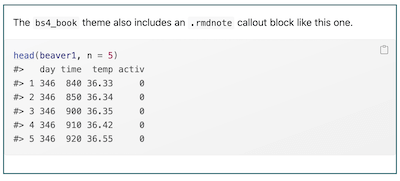
\includegraphics{images/rmd-note} 

}

\caption{A special callout block.}\label{fig:bs4-note}
\end{figure}

可用的区块有 \texttt{.rmdnote}、\texttt{.rmdcaution}、\texttt{.rmdimportant}、\texttt{.rmdtip} 和 \texttt{.rmdwarning}。使用的颜色将基于 Bootstrap 提供的默认颜色,但也可以在你的 \texttt{\_output.yml} 文件中自定义。

\begin{Shaded}
\begin{Highlighting}[]
\AttributeTok{bookdown:}\FunctionTok{:bs4\_book}\KeywordTok{:}
\AttributeTok{  }\FunctionTok{theme}\KeywordTok{:}
\AttributeTok{    }\FunctionTok{primary}\KeywordTok{:}\AttributeTok{ }\StringTok{"\#0d6efd"}\CommentTok{   \# default .rmdnote = blue}
\AttributeTok{    }\FunctionTok{danger}\KeywordTok{:}\AttributeTok{  }\StringTok{"\#dc3545"}\CommentTok{   \# default .rmdcaution = red}
\AttributeTok{    }\FunctionTok{success}\KeywordTok{:}\AttributeTok{ }\StringTok{"\#198754"}\CommentTok{   \# default .rmdimportant = green}
\AttributeTok{    }\FunctionTok{info}\KeywordTok{:}\AttributeTok{    }\StringTok{"\#0dcaf0"}\CommentTok{   \# default .rmdtip = cyan}
\AttributeTok{    }\FunctionTok{warning}\KeywordTok{:}\AttributeTok{ }\StringTok{"\#ffc107"}\CommentTok{   \# default .rmdwarning = yellow}
\end{Highlighting}
\end{Shaded}

对于LaTeX输出,只有这些区块的内容会被显示出来,没有像 HTML 那样的彩色轮廓。用户可以使用自定义环境来定义在 LaTeX 输出时这些区块的外观。参见 \href{https://bookdown.org/yihui/rmarkdown-cookbook/custom-blocks.html}{\emph{R Markdown Cookbook}}以了解如何操作。

\subsubsection{HTML 元数据}\label{html-ux5143ux6570ux636e}

Bookdown 将根据 Pandoc 在 \texttt{index.Rmd} 中设置的变量生成 HTML \texttt{\textless{}meta\textgreater{}} 标签,该部分内容在第 \ref{metadata-for-sharing} 节中进行了描述。此外,\texttt{bs4\_book()} 将创建独特的章节描述,这些描述是由章节的内容自动生成的。你可以查阅 \href{https://github.com/rstudio/bookdown/blob/main/inst/templates/bs4_book.html}{\texttt{bs4\_book} 的 HTML
模板}来了解这些变量的使用细节。

\subsubsection{行内脚注}\label{bs4-book-footnotes}

\texttt{bs4\_book} 使任何脚注显示为在悬停状态下的行内显示,而不是在页面底部的链接项。您可以设置 \texttt{footnotes\_inline\ =\ FALSE} 来选择取消这种行为,并将脚注放在底部。

\begin{Shaded}
\begin{Highlighting}[]
\AttributeTok{bookdown:}\FunctionTok{:bs4\_book}\KeywordTok{:}
\AttributeTok{  }\FunctionTok{footnotes\_inline}\KeywordTok{:}\AttributeTok{ }\CharTok{false}
\end{Highlighting}
\end{Shaded}

\subsubsection{参考文献/书目}\label{ux53c2ux8003ux6587ux732eux4e66ux76ee}

将你的引用文献制作为 \emph{脚注},可以让读者在引用它们的文本附近阅读脚注内容,因为 \texttt{bs4\_book} 默认使脚注在点击时出现在行内。要做到这一点,请下载一个脚注样式的 CSL 文件;我们推荐 \url{https://www.zotero.org/styles/}。例如,你可以从 \href{https://www.zotero.org/styles/?q=id\%3Achicago-fullnote-bibliography}{Zotero} 下载 \texttt{chicago-fullnote-bibliography.csl},然后添加到你的 \texttt{index.Rmd} 中。

\begin{Shaded}
\begin{Highlighting}[]
\FunctionTok{bibliography}\KeywordTok{:}\AttributeTok{ refs.bib}
\FunctionTok{csl}\KeywordTok{:}\AttributeTok{ chicago{-}fullnote{-}bibliography.csl}
\end{Highlighting}
\end{Shaded}

如果你不想在书籍的最后有一个参考文献章节,可以选择在你的 \texttt{index.Rmd} 中添加这一行:

\begin{Shaded}
\begin{Highlighting}[]
\FunctionTok{suppress{-}bibliography}\KeywordTok{:}\AttributeTok{ }\CharTok{true}
\end{Highlighting}
\end{Shaded}

如果你想使用不支持脚注的引用文献样式,参考文献将不会在行内弹出窗口中显示。在这种情况下,你可能希望在你的 \texttt{\_output.yml} 中添加 \texttt{split\_bib} 配置项。

\begin{Shaded}
\begin{Highlighting}[]
\AttributeTok{bookdown:}\FunctionTok{:bs4\_book}\KeywordTok{:}
\AttributeTok{  }\FunctionTok{split\_bib}\KeywordTok{:}\AttributeTok{ }\CharTok{true}
\end{Highlighting}
\end{Shaded}

这样,你的参考书目将被拆分,相关的引用文献项目将被放在每一章的底部,这样读者就不必跳转到不同的参考书目页来查看引用文献的细节。

\subsubsection{指定储存库}\label{ux6307ux5b9aux50a8ux5b58ux5e93}

为你的书籍指定一个源码储存库,让你的读者可以轻松查看每一章的源文件或提出编辑建议。

如果你的书籍有一个名为 \texttt{main} 的默认分支,可以使用。

\begin{Shaded}
\begin{Highlighting}[]
\AttributeTok{bookdown:}\FunctionTok{:bs4\_book}\KeywordTok{:}
\AttributeTok{  }\FunctionTok{repo}\KeywordTok{:}
\AttributeTok{    }\FunctionTok{base}\KeywordTok{:}\AttributeTok{ https://github.com/hadley/ggplot2{-}book}
\AttributeTok{    }\FunctionTok{branch}\KeywordTok{:}\AttributeTok{ main}
\end{Highlighting}
\end{Shaded}

进一步,如果你的书籍位于一个名为 ``book'' 的子目录中,你可以使用:

\begin{Shaded}
\begin{Highlighting}[]
\AttributeTok{bookdown:}\FunctionTok{:bs4\_book}\KeywordTok{:}
\AttributeTok{  }\FunctionTok{repo}\KeywordTok{:}
\AttributeTok{    }\FunctionTok{base}\KeywordTok{:}\AttributeTok{ https://github.com/hadley/ggplot2{-}book}
\AttributeTok{    }\FunctionTok{branch}\KeywordTok{:}\AttributeTok{ main}
\AttributeTok{    }\FunctionTok{subdir}\KeywordTok{:}\AttributeTok{ book}
\end{Highlighting}
\end{Shaded}

默认情况下,如果储存库的 URL 包含 ``github'',它将获得一个 GitHub \href{https://fontawesome.com}{Font Awesome} 图标,否则它将获得一个 GitLab 图标。要使用其他图标,请用正确的前缀来指定,如 \texttt{fas}、\texttt{fab} 等等 (\href{https://fontawesome.com/v5.0/how-to-use/on-the-web/referencing-icons/basic-use}{Font Awesome 5})。

\begin{Shaded}
\begin{Highlighting}[]
\AttributeTok{bookdown:}\FunctionTok{:bs4\_book}\KeywordTok{:}
\AttributeTok{  }\FunctionTok{repo}\KeywordTok{:}
\AttributeTok{    }\FunctionTok{base}\KeywordTok{:}\AttributeTok{ https://github.com/hadley/ggplot2{-}book}
\AttributeTok{    }\FunctionTok{branch}\KeywordTok{:}\AttributeTok{ main}
\AttributeTok{    }\FunctionTok{subdir}\KeywordTok{:}\AttributeTok{ book}
\AttributeTok{    }\FunctionTok{icon}\KeywordTok{:}\AttributeTok{ }\StringTok{"fas fa{-}air{-}freshener"}
\end{Highlighting}
\end{Shaded}

\subsection{默认的 Bootstrap 样式}\label{bootstrap-style}

如果你之前使用过 R Markdown,你应该熟悉 Bootstrap\index{Bootstrap style} 样式 (\url{https://getbootstrap.com}),它是 R Markdown 的 HTML 输出格式的默认样式。\textbf{rmarkdown} 中的输出格式函数是 \texttt{html\_document()},并且我们在 \textbf{bookdown} 中也有一个相应的格式 \texttt{html\_book()},它使用 \texttt{html\_document()} 作为基础格式。你可以在这里阅读 \texttt{html\_book()} 的样例:\url{https://bookdown.org/yihui/bookdown-demo2}。

事实上,\textbf{bookdown} 中有一个更加通用的格式 \texttt{html\_chapters()},\texttt{html\_book()} 只是它的特例:

\begin{Shaded}
\begin{Highlighting}[]
\FunctionTok{html\_chapters}\NormalTok{(}\AttributeTok{toc =} \ConstantTok{TRUE}\NormalTok{, }\AttributeTok{number\_sections =} \ConstantTok{TRUE}\NormalTok{,}
  \AttributeTok{fig\_caption =} \ConstantTok{TRUE}\NormalTok{, }\AttributeTok{lib\_dir =} \StringTok{"libs"}\NormalTok{,}
  \AttributeTok{template =} \FunctionTok{bookdown\_file}\NormalTok{(}\StringTok{"templates/default.html"}\NormalTok{),}
  \AttributeTok{global\_numbering =} \SpecialCharTok{!}\NormalTok{number\_sections,}
  \AttributeTok{pandoc\_args =} \ConstantTok{NULL}\NormalTok{, ...,}
  \AttributeTok{base\_format =}\NormalTok{ rmarkdown}\SpecialCharTok{::}\NormalTok{html\_document,}
  \AttributeTok{split\_bib =} \ConstantTok{TRUE}\NormalTok{, }\AttributeTok{page\_builder =}\NormalTok{ build\_chapter,}
  \AttributeTok{split\_by =} \FunctionTok{c}\NormalTok{(}\StringTok{"section+number"}\NormalTok{, }\StringTok{"section"}\NormalTok{, }\StringTok{"chapter+number"}\NormalTok{, }\StringTok{"chapter"}\NormalTok{, }\StringTok{"rmd"}\NormalTok{, }\StringTok{"none"}\NormalTok{))}
\end{Highlighting}
\end{Shaded}

请注意它有一个 \texttt{base\_format} 参数,接受一个基础输出格式函数,并且 \texttt{html\_book()} 基本上就是 \texttt{html\_chapters(base\_format\ =\ rmarkdown::html\_document)}。\texttt{html\_book()} 的所有参数都传递给 \texttt{html\_chapters()}:

\begin{Shaded}
\begin{Highlighting}[]
\FunctionTok{html\_book}\NormalTok{(...)}
\end{Highlighting}
\end{Shaded}

这意味着你可以使用 \texttt{rmarkdown::html\_document} 的大多数参数,例如 \texttt{toc} (是否展示目录), \texttt{number\_sections}(是否为章节标题标号)等等。类似地,关于可用配置项的完整列表,请查阅 \texttt{rmarkdown::html\_document} 的帮助页面。注意 \texttt{self\_contained} 参数在内部硬编码为 \texttt{FALSE},因此你不能更改这个参数的值。关于 \texttt{split\_by} 参数,我们在之前的章节中已经解释过了。

参数 \texttt{template} 和 \texttt{page\_builder} 是为高级用户准备的,除非你有强烈的定制 HTML 输出的需求,并且 \texttt{rmarkdown::html\_document()} 提供的众多选项仍然无法为你提供想要的效果,否则你不需要理解它们。

如果你想将不同的 HTML 模板传递给 \texttt{template} 参数,则模板必须包括三对 HTML 注释,每条注释必须位于单独的行中:

\begin{itemize}
\tightlist
\item
  \texttt{\textless{}!-\/-bookdown:title:start-\/-\textgreater{}} 和 \texttt{\textless{}!-\/-bookdown:title:end-\/-\textgreater{}} 标记书籍的标题部分。这部分仅放在编译好的书籍的第一页;
\item
  \texttt{\textless{}!-\/-bookdown:toc:start-\/-\textgreater{}} 和 \texttt{\textless{}!-\/-bookdown:toc:end-\/-\textgreater{}} 标记目录部分,这部分将会被放在所有 HTML 页面上;
\item
  \texttt{\textless{}!-\/-bookdown:body:start-\/-\textgreater{}} 和 \texttt{\textless{}!-\/-bookdown:body:end-\/-\textgreater{}} 标记书籍的 HTML 主体,HTML 主体内容将会被划分为多个单独的页面。回想一下,我们合并了所有 R Markdown 或 Markdown 文件,然后将其编译为单个 HTML 文件,并将其拆分;
\end{itemize}

你可以打开默认的 HTML 模板,查看这些注释的插入位置:

\begin{Shaded}
\begin{Highlighting}[]
\NormalTok{bookdown}\SpecialCharTok{:::}\FunctionTok{bookdown\_file}\NormalTok{(}\StringTok{\textquotesingle{}templates/default.html\textquotesingle{}}\NormalTok{)}
\CommentTok{\# you may use file.edit() to open this file}
\end{Highlighting}
\end{Shaded}

一旦你知道 \textbf{bookdown} 在内部如何生成多页 HTML 输出,将更容易理解 \texttt{page\_builder} 参数。它是一个函数,能够使用从上述注释标志中提取的 HTML 片段来合成每个单独的 HTML 页面。\texttt{page\_builder} 的默认值是 \textbf{bookdown} 中的 \texttt{build\_chapter} 函数,其源代码相对简单(忽略 \texttt{button\_link()} 等内部函数):

\begin{Shaded}
\begin{Highlighting}[]
\NormalTok{build\_chapter }\OtherTok{=} \ControlFlowTok{function}\NormalTok{(}
\NormalTok{  head, toc, chapter, link\_prev, link\_next, rmd\_cur, html\_cur, foot}
\NormalTok{) \{}
\NormalTok{  toc }\OtherTok{=} \FunctionTok{add\_toc\_class}\NormalTok{(toc)}
  \FunctionTok{paste}\NormalTok{(}\FunctionTok{c}\NormalTok{(}
\NormalTok{    head,}
    \StringTok{\textquotesingle{}\textless{}div class="row"\textgreater{}\textquotesingle{}}\NormalTok{,}
    \StringTok{\textquotesingle{}\textless{}div class="col{-}sm{-}12"\textgreater{}\textquotesingle{}}\NormalTok{,}
\NormalTok{    toc,}
    \StringTok{\textquotesingle{}\textless{}/div\textgreater{}\textquotesingle{}}\NormalTok{,}
    \StringTok{\textquotesingle{}\textless{}/div\textgreater{}\textquotesingle{}}\NormalTok{,}
    \StringTok{\textquotesingle{}\textless{}div class="row"\textgreater{}\textquotesingle{}}\NormalTok{,}
    \StringTok{\textquotesingle{}\textless{}div class="col{-}sm{-}12"\textgreater{}\textquotesingle{}}\NormalTok{,}
\NormalTok{    chapter,}
    \StringTok{\textquotesingle{}\textless{}p style="text{-}align: center;"\textgreater{}\textquotesingle{}}\NormalTok{,}
    \FunctionTok{button\_link}\NormalTok{(link\_prev, }\StringTok{\textquotesingle{}Previous\textquotesingle{}}\NormalTok{),}
    \FunctionTok{source\_link}\NormalTok{(rmd\_cur, }\AttributeTok{type =} \StringTok{\textquotesingle{}edit\textquotesingle{}}\NormalTok{),}
    \FunctionTok{source\_link}\NormalTok{(rmd\_cur, }\AttributeTok{type =} \StringTok{\textquotesingle{}history\textquotesingle{}}\NormalTok{),}
    \FunctionTok{source\_link}\NormalTok{(rmd\_cur, }\AttributeTok{type =} \StringTok{\textquotesingle{}view\textquotesingle{}}\NormalTok{),}
    \FunctionTok{button\_link}\NormalTok{(link\_next, }\StringTok{\textquotesingle{}Next\textquotesingle{}}\NormalTok{),}
    \StringTok{\textquotesingle{}\textless{}/p\textgreater{}\textquotesingle{}}\NormalTok{,}
    \StringTok{\textquotesingle{}\textless{}/div\textgreater{}\textquotesingle{}}\NormalTok{,}
    \StringTok{\textquotesingle{}\textless{}/div\textgreater{}\textquotesingle{}}\NormalTok{,}
\NormalTok{    foot}
\NormalTok{  ), }\AttributeTok{collapse =} \StringTok{\textquotesingle{}}\SpecialCharTok{\textbackslash{}n}\StringTok{\textquotesingle{}}\NormalTok{)}
\NormalTok{\}}
\end{Highlighting}
\end{Shaded}

基本上,这个函数使用许多组件,如 HTML 头部、目录、章节正文等,它将返回一个字符串,该字符串是完整 HTML 页面的 HTML 源代码。你可以使用诸如 \texttt{gsub()} 和 \texttt{paste()} 之类的文本处理函数来操作此函数中的所有组件。

默认的页面生成器所做的是将目录放在第一行,正文放在第二行,导航按钮放在正文底部,并将它们与 HTML 头部和底部连接起来。下面是 HTML 源代码的一个简要示例,可以帮助你理解 \texttt{build\_chapter()} 的输出:

\begin{Shaded}
\begin{Highlighting}[]
\DataTypeTok{\textless{}}\KeywordTok{html}\DataTypeTok{\textgreater{}}
  \DataTypeTok{\textless{}}\KeywordTok{head}\DataTypeTok{\textgreater{}}
    \DataTypeTok{\textless{}}\KeywordTok{title}\DataTypeTok{\textgreater{}}\NormalTok{一本好书}\DataTypeTok{\textless{}/}\KeywordTok{title}\DataTypeTok{\textgreater{}}
  \DataTypeTok{\textless{}/}\KeywordTok{head}\DataTypeTok{\textgreater{}}
  \DataTypeTok{\textless{}}\KeywordTok{body}\DataTypeTok{\textgreater{}}
  
    \DataTypeTok{\textless{}}\KeywordTok{div}\OtherTok{ class}\OperatorTok{=}\StringTok{"row"}\DataTypeTok{\textgreater{}}\NormalTok{目录}\DataTypeTok{\textless{}/}\KeywordTok{div}\DataTypeTok{\textgreater{}}
    
    \DataTypeTok{\textless{}}\KeywordTok{div}\OtherTok{ class}\OperatorTok{=}\StringTok{"row"}\DataTypeTok{\textgreater{}}
\NormalTok{      章节主体}
      \DataTypeTok{\textless{}}\KeywordTok{p}\DataTypeTok{\textgreater{}}
        \DataTypeTok{\textless{}}\KeywordTok{button}\DataTypeTok{\textgreater{}}\NormalTok{上一章}\DataTypeTok{\textless{}/}\KeywordTok{button}\DataTypeTok{\textgreater{}}
        \DataTypeTok{\textless{}}\KeywordTok{button}\DataTypeTok{\textgreater{}}\NormalTok{下一章}\DataTypeTok{\textless{}/}\KeywordTok{button}\DataTypeTok{\textgreater{}}
      \DataTypeTok{\textless{}/}\KeywordTok{p}\DataTypeTok{\textgreater{}}
    \DataTypeTok{\textless{}/}\KeywordTok{div}\DataTypeTok{\textgreater{}}
  
  \DataTypeTok{\textless{}/}\KeywordTok{body}\DataTypeTok{\textgreater{}}
\DataTypeTok{\textless{}/}\KeywordTok{html}\DataTypeTok{\textgreater{}}
\end{Highlighting}
\end{Shaded}

对于所有 HTML 页面,主要的区别在于章节主体,其它大部分元素是相同的。\texttt{html\_book()} 的默认输出将在 \texttt{\textless{}head\textgreater{}} 标签中包括 Bootstrap CSS 和 JavaScript 文件。

目录常用于导航。在 GitBook 样式中,目录显示在侧边栏中。对于 Bootstrap 样式,我们没有对它应用特殊样式,因此它显示为普通的无序列表(在 HTML 标签 \texttt{\textless{}ul\textgreater{}} 中)。使用某些 CSS 技术可以轻松地将此列表转为导航栏。在这个软件包中我们已经提供了一个 CSS 文件 \texttt{toc.css},你可以在这里找到它:\url{https://github.com/rstudio/bookdown/blob/master/inst/examples/css/toc.css}

你可以复制这个文件导你的书籍的根目录,然后通过 \texttt{css} 配置项应用到 HTML 输出,例如:

\begin{Shaded}
\begin{Highlighting}[]
\PreprocessorTok{{-}{-}{-}}
\FunctionTok{output}\KeywordTok{:}
\AttributeTok{  bookdown:}\FunctionTok{:html\_book}\KeywordTok{:}
\AttributeTok{    }\FunctionTok{toc}\KeywordTok{:}\AttributeTok{ }\CharTok{true}
\AttributeTok{    }\FunctionTok{css}\KeywordTok{:}\AttributeTok{ toc.css}
\PreprocessorTok{{-}{-}{-}}
\end{Highlighting}
\end{Shaded}

如果你在网上稍微搜索一下,就能找到许多可能的方法将 \texttt{\textless{}ul\textgreater{}} 列表变成导航菜单,你可以选择你喜欢的菜单样式。我们刚才提到的 \texttt{toc.css} 是一种在黑色背景上有白色菜单文本的样式,并且支持子菜单(例如,节标题显示为章标题下的下拉菜单)。

事实上,如果你把 \texttt{theme} 选项设置为 \texttt{null},就可以在 \texttt{html\_document()} 中摆脱 Bootstrap 样式,你可以自由地使用 \texttt{css} 选项在 HTML 输出中应用任意的样式(如果你想在 HTML 头部/底部中包含任意的内容,还可以使用 \texttt{includes} 选项)。

\subsection{Tufte 样式}\label{tufte-style}

和 Bootstrap 样式一样,Tufte\index{Tufte style} 样式由输出格式 \texttt{tufte\_html\_book()} 提供,这也是 \texttt{html\_chapters()} 的一个特例,使用 \texttt{tufte::tufte\_html()} 作为基础格式。如果你不熟悉 Tufte 样式,请查阅 \textbf{tufte} 软件包\citep{R-tufte}。你可以在这里阅读一个 \texttt{tufte\_html\_book()} 的例子:\url{https://bookdown.org/yihui/bookdown-demo3/}。

基本上,它是一个左边是主栏,右边是边栏的布局。内容主体在主栏中,边栏用来放置脚注 (footnotes)、边注 (margin notes)、参考文献 (references) 和边栏图片 (margin figures) 等。

\texttt{tufte\_html\_book()} 的所有参数的含义与 \texttt{html\_book()} 完全相同,例如,你同样也可以通过 \texttt{css} 配置项定制 CSS。然而,有一些元素是 Tufte 风格所特有的,如边注 (margin notes)、边栏图片 (margin figures) 和全宽图片 (full-width figures)。这些元素需要特殊的语法来生成;请查阅 \textbf{tufte} 软件包的文档。请注意,你不需要对脚注和参考文献做任何特殊处理(只需使用正常的 Markdown 语法 \texttt{\^{}{[}footnote{]}} 和 \texttt{{[}@citation{]}}),因为它们会被自动放到页边。一个关于 \texttt{tufte\_html\_book} 格式的简短 YAML 示例如下:

\begin{Shaded}
\begin{Highlighting}[]
\PreprocessorTok{{-}{-}{-}}
\FunctionTok{output}\KeywordTok{:}
\AttributeTok{  bookdown:}\FunctionTok{:tufte\_html\_book}\KeywordTok{:}
\AttributeTok{    }\FunctionTok{toc}\KeywordTok{:}\AttributeTok{ }\CharTok{true}
\AttributeTok{    }\FunctionTok{css}\KeywordTok{:}\AttributeTok{ toc.css}
\PreprocessorTok{{-}{-}{-}}
\end{Highlighting}
\end{Shaded}

\section{LaTeX/PDF}\label{latexpdf}

我们强烈建议你在撰写书籍时使用 HTML 输出格式,而不是 LaTeX\index{LaTeX},因为你将不会因为排版细节而分心,如果经常查看书籍的 PDF 输出就会知道,排版细节会给你带来很多麻烦。把仔细排版的工作留到最后(最好在真正完成书籍的内容之后)。

LaTeX/PDF 输出格式是由 \textbf{bookdown} 中的 \texttt{pdf\_book()} 提供的。\texttt{pdf\_book()} 和 \textbf{rmarkdown} 中的 \texttt{pdf\_document()} 格式之间没有明显的区别。\texttt{pdf\_book()} 的主要目的是解决使用第 \ref{figures}、\ref{tables} 和 \ref{cross-references} 节中描述的语法编写的标签和交叉引用。如果你希望书籍的唯一输出格式是 LaTeX/PDF,则可以使用 LaTeX 特有的语法,例如使用 \texttt{\textbackslash{}label\{\}} 来标记图片/表格/章节,使用 \texttt{\textbackslash{}ref\{\}} 通过它们的标签来交叉引用,因为 Pandoc 支持在 Markdown 中使用 LaTeX 命令。然而,LaTeX 语法不能移植到其他输出格式,如 HTML 和电子书。这就是为什么我们为标签引入了 \texttt{(\textbackslash{}\#label)} 语法,为交叉引用引入了 \texttt{\textbackslash{}@ref(label)} 语法。

有一些顶级 YAML 配置项将被应用于 LaTeX 输出。对于一本书,你可以把默认的文档类别改为 \texttt{book}(默认是 \texttt{artical}),并指定出版商要求的参考文献样式。下面是一个一个简短的 YAML 示例。

\begin{Shaded}
\begin{Highlighting}[]
\PreprocessorTok{{-}{-}{-}}
\FunctionTok{documentclass}\KeywordTok{:}\AttributeTok{ book}
\FunctionTok{bibliography}\KeywordTok{:}\AttributeTok{ }\KeywordTok{[}\AttributeTok{book.bib}\KeywordTok{,}\AttributeTok{ packages.bib}\KeywordTok{]}
\FunctionTok{biblio{-}style}\KeywordTok{:}\AttributeTok{ apalike}
\PreprocessorTok{{-}{-}{-}}
\end{Highlighting}
\end{Shaded}

LaTeX 输出格式还有大量的 YAML 配置项可以使用,如纸张大小、字体大小、页边距、行间距、字体族等等。关于配置项的完整列表,请参见 \url{http://pandoc.org/MANUAL.html\#variables-for-latex}。

\texttt{pdf\_book()} 格式与 \texttt{html\_book()} 一样是一种通用格式,它也有一个 \texttt{base\_format} 参数。

\begin{Shaded}
\begin{Highlighting}[]
\FunctionTok{pdf\_book}\NormalTok{(}\AttributeTok{toc =} \ConstantTok{TRUE}\NormalTok{, }\AttributeTok{number\_sections =} \ConstantTok{TRUE}\NormalTok{,}
  \AttributeTok{fig\_caption =} \ConstantTok{TRUE}\NormalTok{, }\AttributeTok{pandoc\_args =} \ConstantTok{NULL}\NormalTok{, ...,}
  \AttributeTok{base\_format =}\NormalTok{ rmarkdown}\SpecialCharTok{::}\NormalTok{pdf\_document,}
  \AttributeTok{toc\_unnumbered =} \ConstantTok{TRUE}\NormalTok{, }\AttributeTok{toc\_appendix =} \ConstantTok{FALSE}\NormalTok{,}
  \AttributeTok{toc\_bib =} \ConstantTok{FALSE}\NormalTok{, }\AttributeTok{quote\_footer =} \ConstantTok{NULL}\NormalTok{,}
  \AttributeTok{highlight\_bw =} \ConstantTok{FALSE}\NormalTok{)}
\end{Highlighting}
\end{Shaded}

你可以将 \texttt{base\_format} 函数改成其他的输出格式函数,\textbf{bookdown} 提供了一个简单的封装函数 \texttt{tufte\_book2()},基本上就是 \texttt{pdf\_book(base\_format\ =\ tufte::tufte\_book)},用 Tufte 的 PDF 样式来制作一本 PDF 书籍(类似地,详情请见 \textbf{tufte} 软件包)。

\section{电子书}\label{ux7535ux5b50ux4e66}

目前 \textbf{bookdown} 支持 EPUB\index{EPUB} 和 MOBI\index{MOBI} 两种电子书\index{e-book}格式。这些格式的书籍可以在智能手机、平板电脑或者是 Kindle 等特殊的电子阅读器上阅读。

\subsection{EPUB}\label{epub}

你可以使用 \texttt{epub\_book()} 格式来创建一本 EPUB 书籍。它的一些配置项与 \texttt{rmarkdown::html\_document()} 相同:

\begin{Shaded}
\begin{Highlighting}[]
\FunctionTok{epub\_book}\NormalTok{(}\AttributeTok{fig\_width =} \DecValTok{5}\NormalTok{, }\AttributeTok{fig\_height =} \DecValTok{4}\NormalTok{, }\AttributeTok{dev =} \StringTok{"png"}\NormalTok{,}
  \AttributeTok{fig\_caption =} \ConstantTok{TRUE}\NormalTok{, }\AttributeTok{number\_sections =} \ConstantTok{TRUE}\NormalTok{,}
  \AttributeTok{toc =} \ConstantTok{FALSE}\NormalTok{, }\AttributeTok{toc\_depth =} \DecValTok{3}\NormalTok{, }\AttributeTok{stylesheet =} \ConstantTok{NULL}\NormalTok{,}
  \AttributeTok{cover\_image =} \ConstantTok{NULL}\NormalTok{, }\AttributeTok{metadata =} \ConstantTok{NULL}\NormalTok{,}
  \AttributeTok{chapter\_level =} \DecValTok{1}\NormalTok{,}
  \AttributeTok{epub\_version =} \FunctionTok{c}\NormalTok{(}\StringTok{"epub3"}\NormalTok{, }\StringTok{"epub"}\NormalTok{, }\StringTok{"epub2"}\NormalTok{),}
  \AttributeTok{md\_extensions =} \ConstantTok{NULL}\NormalTok{,}
  \AttributeTok{global\_numbering =} \SpecialCharTok{!}\NormalTok{number\_sections,}
  \AttributeTok{pandoc\_args =} \ConstantTok{NULL}\NormalTok{, }\AttributeTok{template =} \StringTok{"default"}\NormalTok{)}
\end{Highlighting}
\end{Shaded}

关闭 \texttt{toc} 选项是因为电子书阅读器通常可以从书中自动找出目录,所以没有必要为目录多增加几页。有几个专门针对 EPUB 的配置项:

\begin{itemize}
\tightlist
\item
  \texttt{stylesheet}: 它类似于 HTML 输出格式中的 \texttt{css} 配置项,你可以用 CSS 来定制元素的外观。
\item
  \texttt{cover\_image}: 书籍封面图片的路径。
\item
  \texttt{metadata}: 书籍元数据所在 XML 文件的路径(更多细节请见 Pandoc 文档)。
\item
  \texttt{chapter\_level}: 在内部,一本 EPUB 书籍是一系列的``章节''文件,这个配置项决定了书籍在何种级别上被分割成这些文件。这类似于我们在第 \ref{html} 节中提到的 HTML 输出格式的 \texttt{split\_by} 参数,但是 EPUB 书籍是一个单一的文件,你不会直接看到这些``章节''文件。默认的级别是第一级,如果你把它设置为 2,意味着这本书在内部会按节划分文件来组织,这可能会使得书籍加载更快。
\item
  \texttt{epub\_version}: EPUB 的第 3 版或第 2 版。
\end{itemize}

EPUB 书籍本质上是 HTML 页面的集合,例如,你可以将 CSS 规则应用于其元素、嵌入图像、插入数学表达式(因为 EPUB 部分支持 MathML)等等。第 \ref{components} 节中提到的图片/表格标题、交叉引用、自定义区块和引用也适用于 EPUB。你可以将本书的 EPUB 输出与 HTML 输出进行比较,你将看到二者唯一的主要区别是视觉外观。

有几个 EPUB 阅读器可以阅读书籍,包括 Calibre (\url{https://www.calibre-ebook.com})、苹果的 iBooks 和谷歌的 Play Books。

\subsection{MOBI}\label{mobi}

MOBI 电子书可以在亚马逊的 Kindle 设备上阅读。Pandoc 本身不支持 MOBI 输出,但你可以使用第三方工具将 EPUB 转换为 MOBI。其中一种工具是 Calibre\index{Calibre}。Calibre 是开源并且免费的,并且支持更多格式之间的相互转换。例如,你可以将 HTML 转换成 EPUB,将 Word 文档转换成 MOBI 等等。在 \textbf{bookdown} 中的函数 \texttt{calibre()} 是 Calibre 中命令行工具 \texttt{ebook-convert} 的封装函数。你需要确保通过环境变量 \texttt{PATH} 可以找到可执行的 \texttt{ebook-convert}。如果你使用 macOS,你可以通过 \texttt{brew\ cask\ install\ calibre} 命令用 Homebrew (\url{https://brew.sh}) 安装 Calibre,所以你不需要担心 \texttt{PATH} 问题。

\section{单个文档}\label{a-single-document}

有时你可能不想写一本书,而是想写一篇长篇文章或报告。通常你要做的是使用特定的输出格式函数调用 \texttt{rmarkdown::render()}\index{rmarkdown::render()}。这种情况下缺少的主要功能是图片/表格/方程的自动编号,以及对图片/表格/方程/章节的交叉引用。我们已经将这些特性从 \textbf{bookdown} 中分解出来,这样你就可以使用它们而无需准备一本包含多个 Rmd 文件的书籍。

函数 \texttt{html\_document2()}、\texttt{tufte\_html2()}、\texttt{pdf\_document2()}、\texttt{word\_document2()}、\texttt{tufte\_handout2()} 和 \texttt{tufte\_book2()} 就是为此目的而设计的。如果使用这些输出格式渲染一份 R Markdown 文档,例如 \texttt{bookdown::html\_document2},你将能够对图片/表格自动编号,并能够使用第 \ref{components} 章描述的语法在单个 HTML 页面中对它们进行交叉引用。

下面是单个 Rmd 文件的 YAML 元数据中这些输出格式的几个例子(你也可以把这些格式添加到 \texttt{\_output.yml} 文件中)。

\begin{Shaded}
\begin{Highlighting}[]
\FunctionTok{output}\KeywordTok{:}
\AttributeTok{  bookdown:}\FunctionTok{:html\_document2}\KeywordTok{:}\AttributeTok{ default}
\AttributeTok{  bookdown:}\FunctionTok{:pdf\_document2}\KeywordTok{:}
\AttributeTok{    }\FunctionTok{keep\_tex}\KeywordTok{:}\AttributeTok{ }\CharTok{true}
\AttributeTok{  bookdown:}\FunctionTok{:word\_document2}\KeywordTok{:}
\AttributeTok{    }\FunctionTok{toc}\KeywordTok{:}\AttributeTok{ }\CharTok{true}
\end{Highlighting}
\end{Shaded}

上面的 HTML 和 PDF 输出格式函数基本上是对输出格式 \texttt{bookdown::html\_book} 和 \texttt{bookdown::pdf\_book} 的封装,其意义在于它们改变了 \texttt{base\_format} 参数。例如,你可以查阅 \texttt{pdf\_document2} 的源代码。

\begin{Shaded}
\begin{Highlighting}[]
\NormalTok{bookdown}\SpecialCharTok{::}\NormalTok{pdf\_document2}
\end{Highlighting}
\end{Shaded}

\begin{verbatim}
## function (...) 
## {
##     pdf_book(..., base_format = rmarkdown::pdf_document)
## }
## <bytecode: 0x0000017bd71e85f8>
## <environment: namespace:bookdown>
\end{verbatim}

在你知道这个事实后,你可以通过使用适当的 \texttt{base\_format} 将同样的想法应用于其他输出格式。例如,你可以通过使用 YAML 元数据将 \textbf{bookdown} 的功能移植到 \textbf{rticles} 软件包\citep{R-rticles}中的 \texttt{jss\_article} 格式。

\begin{Shaded}
\begin{Highlighting}[]
\FunctionTok{output}\KeywordTok{:}
\AttributeTok{  bookdown:}\FunctionTok{:pdf\_book}\KeywordTok{:}
\AttributeTok{    }\FunctionTok{base\_format}\KeywordTok{:}\AttributeTok{ rticles::jss\_article}
\end{Highlighting}
\end{Shaded}

然后你就可以使用我们在第 \ref{components} 章中介绍的所有功能了。

尽管 \texttt{gitbook()} 格式主要是为书籍设计的,但实际上你也可以将其应用于单个 R Markdown 文档。唯一不同的是,在单页输出上不会有搜索按钮,因为你可以简单地使用网络浏览器的搜索工具来查找文本(例如使用 \texttt{Ctrl\ +\ F} 或 \texttt{Command\ +\ F})。你也可以把选项 \texttt{split\_by} 设置为 \texttt{none},这样只会生成一个输出页面,在这种情况下不会有任何导航按钮,因为没有其他页面可以导航。如果你愿意,仍然可以生成多页 HTML 文件。当只生成单一的输出页面时,另一个你可能想使用的配置项是 \texttt{self\_contained\ =\ TRUE}。

\chapter{定制化}\label{customization}

正如我们在本书的开头中所提到的,你应该对 R Markdown 有一些基本的了解,并且我们一直在重点介绍 \textbf{bookdown} 而不是 \textbf{rmarkdown} 的特性。事实上,R Markdown 是高度可定制的,你可以使用许多选项来定制输出文档。根据你希望自定义输出文档的程度,你可以在 YAML 元数据中使用一些简单的选项,或者只替换整个 Pandoc 模板。

\section{YAML 选项}\label{yaml-options}

\index{YAML}  对于大多数类型的输出格式来说,你可以使用特定格式的 \texttt{highlight} 选项自定义语法高亮样式,可用的样式为 \texttt{default}、\texttt{tango}、\texttt{pygments}、\texttt{kate}、\texttt{monochrome}、\texttt{espresso}、\texttt{zenburn}、\texttt{haddock} 和 \texttt{breezedark}。例如,你可以为 \texttt{gitbook} 格式选择 \texttt{tango} 样式:

\begin{Shaded}
\begin{Highlighting}[]
\PreprocessorTok{{-}{-}{-}}
\FunctionTok{output}\KeywordTok{:}
\AttributeTok{  bookdown:}\FunctionTok{:gitbook}\KeywordTok{:}
\AttributeTok{    }\FunctionTok{highlight}\KeywordTok{:}\AttributeTok{ tango}
\PreprocessorTok{{-}{-}{-}}
\end{Highlighting}
\end{Shaded}

对于 HTML\index{HTML} 输出格式,你最有可能使用 \texttt{css} 选项来提供自己的 CSS\index{CSS} 样式表,以自定义 HTML 元素的外观。有一个 \texttt{includes} 选项能够适用于更多格式,包括 HTML 和 LaTeX。\texttt{includes} 选项允许你在输出文档之前和/或之后插入任意自定义的内容。它有三个子选项:\texttt{in\_header}、\texttt{before\_body} 和 \texttt{after\_body}。你需要了解 HTML 或 LaTeX 文档的基本结构才能理解这些选项。HTML 文件源文本如下所示:

\begin{Shaded}
\begin{Highlighting}[]
\DataTypeTok{\textless{}}\KeywordTok{html}\DataTypeTok{\textgreater{}}
  
  \DataTypeTok{\textless{}}\KeywordTok{head}\DataTypeTok{\textgreater{}}
  \CommentTok{\textless{}!{-}{-} 这里放置首部内容,例如 CSS 和 JS {-}{-}\textgreater{}}
  \DataTypeTok{\textless{}/}\KeywordTok{head}\DataTypeTok{\textgreater{}}
  
  \DataTypeTok{\textless{}}\KeywordTok{body}\DataTypeTok{\textgreater{}}
  \CommentTok{\textless{}!{-}{-} 这里放置正文内容 {-}{-}\textgreater{}}
  \DataTypeTok{\textless{}/}\KeywordTok{body}\DataTypeTok{\textgreater{}}

\DataTypeTok{\textless{}/}\KeywordTok{html}\DataTypeTok{\textgreater{}}
\end{Highlighting}
\end{Shaded}

\texttt{in\_header} 选项接受一个文件路径然后将文件内容插入到 \texttt{\textless{}head\textgreater{}} 标签之间。\texttt{before\_body} 所指文件将会被插入到 \texttt{\textless{}body\textgreater{}} 标签的正下方,\texttt{after\_body} 所指文件将会被插入到 \texttt{\textless{}/body\textgreater{}} 标签之前。

一个 LaTeX\index{LaTeX} 源文档有着相似的结构:

\begin{Shaded}
\begin{Highlighting}[]
\BuiltInTok{\textbackslash{}documentclass}\NormalTok{\{}\ExtensionTok{book}\NormalTok{\}}

\CommentTok{\% LaTeX 导言 (preamble)}
\CommentTok{\% 这里插入 in\_header}

\KeywordTok{\textbackslash{}begin}\NormalTok{\{}\ExtensionTok{document}\NormalTok{\}}
\CommentTok{\% 这里插入 before\_body}

\CommentTok{\% 这里是正文内容}

\CommentTok{\% 这里插入 after\_body}
\KeywordTok{\textbackslash{}end}\NormalTok{\{}\ExtensionTok{document}\NormalTok{\}}
\end{Highlighting}
\end{Shaded}

\texttt{includes} 选项非常有用且使用灵活。对于 HTML 输出,它意味着你能够将任意 HTML 代码插入到输出中。例如,当你在 HTML 输出中通过 MathJax\index{MathJax} 库渲染 LaTeX 数学表达式,并希望方程编号显示在左侧(默认显示在右侧),你可以创建一个包含有以下代码的文本文件:

\begin{Shaded}
\begin{Highlighting}[]
\DataTypeTok{\textless{}}\KeywordTok{script}\OtherTok{ type=}\StringTok{"text/x{-}mathjax{-}config"}\DataTypeTok{\textgreater{}}
\NormalTok{MathJax}\OperatorTok{.}\AttributeTok{Hub}\OperatorTok{.}\FunctionTok{Config}\NormalTok{(\{}
  \DataTypeTok{TeX}\OperatorTok{:}\NormalTok{ \{ }\DataTypeTok{TagSide}\OperatorTok{:} \StringTok{"left"}\NormalTok{ \}}
\NormalTok{\})}\OperatorTok{;}
\DataTypeTok{\textless{}/}\KeywordTok{script}\DataTypeTok{\textgreater{}}
\end{Highlighting}
\end{Shaded}

让我们假设文件名为 \texttt{mathjax-number.html},并且它位于你的书籍的根目录下(包含有你的全部 Rmd 文件的目录)。你可以通过 \texttt{in\_header} 选项将该文件插入到 HTML 首部,例如:

\begin{Shaded}
\begin{Highlighting}[]
\PreprocessorTok{{-}{-}{-}}
\FunctionTok{output}\KeywordTok{:}
\AttributeTok{  bookdown:}\FunctionTok{:gitbook}\KeywordTok{:}
\AttributeTok{    }\FunctionTok{includes}\KeywordTok{:}
\AttributeTok{      }\FunctionTok{in\_header}\KeywordTok{:}\AttributeTok{ mathjax{-}number.html}
\PreprocessorTok{{-}{-}{-}}
\end{Highlighting}
\end{Shaded}

另一个例子是在 HTML 页面上启用评论区或讨论区。有这么几种可能的选择,例如:Disqus (\url{https://disqus.com}) 或 Hypothesis (\url{https://hypothes.is})。这些服务可以通过 \texttt{includes} 选项轻松地嵌入到你的 HTML 书籍中(有关更多详细信息,请参阅第 \ref{collaboration} 节)。

类似地,如果你熟悉 LaTeX,则可以在导言 (preamble) 中添加任意 LaTeX 代码。这意味着你可以使用任何 LaTeX 软件包,并为书籍设置任何软件包选项。例如,本书通过 \texttt{in\_header} 选项使用了更多的 LaTeX 软件包,如 \textbf{booktabs}(用于更美观的表格)和 \textbf{longtable}(用于跨多个页面的表格),并对图形环境中的链接不起作用的 XeLeTeX 问题进行了修复:

\begin{quote}
中文版还使用了 \textbf{ctex} 软件包以在 PDF 输出中渲染中文字符。
\end{quote}

\begin{Shaded}
\begin{Highlighting}[]
\BuiltInTok{\textbackslash{}usepackage}\NormalTok{\{}\ExtensionTok{booktabs}\NormalTok{\}}
\BuiltInTok{\textbackslash{}usepackage}\NormalTok{\{}\ExtensionTok{longtable}\NormalTok{\}}

\FunctionTok{\textbackslash{}ifxetex}
  \BuiltInTok{\textbackslash{}usepackage}\NormalTok{\{}\ExtensionTok{letltxmacro}\NormalTok{\}}
  \FunctionTok{\textbackslash{}setlength}\NormalTok{\{}\FunctionTok{\textbackslash{}XeTeXLinkMargin}\NormalTok{\}\{1pt\}}
  \FunctionTok{\textbackslash{}LetLtxMacro\textbackslash{}SavedIncludeGraphics\textbackslash{}includegraphics}
  \FunctionTok{\textbackslash{}def\textbackslash{}includegraphics}\NormalTok{\#1\#\{}\CommentTok{\% \#1 catches optional stuff (star/opt. arg.)}
    \FunctionTok{\textbackslash{}IncludeGraphicsAux}\NormalTok{\{\#1\}}\CommentTok{\%}
\NormalTok{  \}}\CommentTok{\%}
  \FunctionTok{\textbackslash{}newcommand*}\NormalTok{\{}\ExtensionTok{\textbackslash{}IncludeGraphicsAux}\NormalTok{\}[2]\{}\CommentTok{\%}
    \FunctionTok{\textbackslash{}XeTeXLinkBox}\NormalTok{\{}\CommentTok{\%}
      \FunctionTok{\textbackslash{}SavedIncludeGraphics}\NormalTok{\#1\{\#2\}}\CommentTok{\%}
\NormalTok{    \}}\CommentTok{\%}
\NormalTok{  \}}\CommentTok{\%}
\FunctionTok{\textbackslash{}fi}
\end{Highlighting}
\end{Shaded}

上述 LaTeX 代码保存在文件 \texttt{preamble.tex} 中,而书籍的 YAML 元数据如下所示:

\begin{Shaded}
\begin{Highlighting}[]
\PreprocessorTok{{-}{-}{-}}
\FunctionTok{output}\KeywordTok{:}
\AttributeTok{  bookdown:}\FunctionTok{:pdf\_book}\KeywordTok{:}
\AttributeTok{    }\FunctionTok{includes}\KeywordTok{:}
\AttributeTok{      }\FunctionTok{in\_header}\KeywordTok{:}\AttributeTok{ preamble.tex}
\PreprocessorTok{{-}{-}{-}}
\end{Highlighting}
\end{Shaded}

\section{更换主题}\label{ux66f4ux6362ux4e3bux9898}

有时你可能想要更改输出的整体主题,这通常可以通过上一节叙述的 \texttt{in\_header} 选项或 \texttt{css} 选项(如果输出格式为 HTML)来完成。一些输出格式有它们独特的主题,例如 \texttt{gitbook}、\texttt{tufte\_html\_book} 和 \texttt{tufte\_book2},而你可能不想过多地自定义这些主题。相比之下,输出格式 \texttt{html\_book()} 和 \texttt{pdf\_book} 不受到特定主题的约束,更具有定制性。

如第 \ref{bootstrap-style} 节所述,\texttt{html\_book()} 的默认样式是 Bootstrap 样式。Bootstrap 样式实际上有一些可以使用的内置主题,包括 \texttt{default}、\texttt{bootstrap}、\texttt{cerulean}、\texttt{cosmo}、\texttt{darkly}、\texttt{flatly}、\texttt{journal}、\texttt{lumen}、\texttt{paper}、\texttt{readable}、\texttt{sandstone}、\texttt{simplex}、\texttt{spacelab}、\texttt{united} 和 \texttt{yeti}。你可以通过 \texttt{theme} 选项设定主题,例如:

\begin{Shaded}
\begin{Highlighting}[]
\PreprocessorTok{{-}{-}{-}}
\FunctionTok{output}\KeywordTok{:}
\AttributeTok{  bookdown:}\FunctionTok{:html\_book}\KeywordTok{:}
\AttributeTok{    }\FunctionTok{theme}\KeywordTok{:}\AttributeTok{ united}
\PreprocessorTok{{-}{-}{-}}
\end{Highlighting}
\end{Shaded}

如果你不喜欢上述任何一个 Bootstrap 主题,你可以将 \texttt{theme} 设置为 \texttt{null},然后通过 \texttt{css} 或 \texttt{includes} 选项应用你自己的 CSS。

对于 \texttt{pdf\_book()},除了上一节提到的 \texttt{in\_header} 选项,另一个方法是改变文档类 (document calss)。对于书籍来说有许多可用的 LaTeX 类,例如 \textbf{memoir} (\url{https://www.ctan.org/pkg/memoir})、\textbf{amsbook} (\url{https://www.ctan.org/pkg/amsbook})、KOMA-Script (\url{https://www.ctan.org/pkg/koma-script}) 等等。以下是在 YAML 元数据中指定 KOMA-Script 软件包中的 \texttt{srcbook} 类的一个简要的示例:

\begin{Shaded}
\begin{Highlighting}[]
\PreprocessorTok{{-}{-}{-}}
\FunctionTok{documentclass}\KeywordTok{:}\AttributeTok{ scrbook}
\FunctionTok{output}\KeywordTok{:}
\AttributeTok{  bookdown:}\FunctionTok{:pdf\_book}\KeywordTok{:}
\AttributeTok{    }\FunctionTok{template}\KeywordTok{:}\AttributeTok{ }\CharTok{null}
\PreprocessorTok{{-}{-}{-}}
\end{Highlighting}
\end{Shaded}

一些出版商(例如 Springer 和 Chapman \& Hall/CRC)有他们自己的 LaTeX 样式或类文件。你可以尝试更改 \texttt{documentclass} 选项来使用他们的文档类,尽管通常情况下并非如此简单。你最终可能会使用 \texttt{in\_header},甚至设计一个自定义的 Pandoc LaTeX 模板来容纳这些文档类。

请注意,当你更改 \texttt{documentclass} 时,你可能会指定一个额外的 Pandoc 参数 \texttt{-\/-top-level-division=chapter} 以便 Pandoc 知道应该将第一级标题视为章而不是小节(这是在 \texttt{documentclass} 为 \texttt{book} 时的默认值),例如:

\begin{Shaded}
\begin{Highlighting}[]
\FunctionTok{documentclass}\KeywordTok{:}\AttributeTok{ krantz}
\FunctionTok{output}\KeywordTok{:}
\AttributeTok{  bookdown:}\FunctionTok{:pdf\_book}\KeywordTok{:}
\AttributeTok{    }\FunctionTok{pandoc\_args}\KeywordTok{:}\AttributeTok{ {-}{-}top{-}level{-}division=chapter}
\end{Highlighting}
\end{Shaded}

\section{模板}\label{ux6a21ux677f}

当 Pandoc 将 Markdown 转换为另一种输出格式时,它在幕后使用模板\index{Pandoc template}。模板是一个纯文本文件,其中包含一些格式为 \texttt{\$variable\$} 的变量。这些变量将由 Pandoc 生成的值替换。下面是一个非常简短的 HTML 输出模板:

\begin{Shaded}
\begin{Highlighting}[]
\DataTypeTok{\textless{}}\KeywordTok{html}\DataTypeTok{\textgreater{}}
  \DataTypeTok{\textless{}}\KeywordTok{head}\DataTypeTok{\textgreater{}}
    \DataTypeTok{\textless{}}\KeywordTok{title}\DataTypeTok{\textgreater{}}\NormalTok{$title$}\DataTypeTok{\textless{}/}\KeywordTok{title}\DataTypeTok{\textgreater{}}
  \DataTypeTok{\textless{}/}\KeywordTok{head}\DataTypeTok{\textgreater{}}
  
  \DataTypeTok{\textless{}}\KeywordTok{body}\DataTypeTok{\textgreater{}}
\NormalTok{  $body$}
  \DataTypeTok{\textless{}/}\KeywordTok{body}\DataTypeTok{\textgreater{}}
\DataTypeTok{\textless{}/}\KeywordTok{html}\DataTypeTok{\textgreater{}}
\end{Highlighting}
\end{Shaded}

它有两个变量 \texttt{title} 和 \texttt{body}。\texttt{title} 的值来自 YAML 元数据的 \texttt{title} 字段,\texttt{body} 是从 Markdown 输入文档的正文生成的 HTML 代码。例如,假设我们有一个 Markdown 文档:

\begin{Shaded}
\begin{Highlighting}[]
\CommentTok{{-}{-}{-}}
\AnnotationTok{title:}\CommentTok{ 一本好书}
\CommentTok{{-}{-}{-}}

\FunctionTok{\# 简介}

\NormalTok{这是一本**优秀的**书!}
\end{Highlighting}
\end{Shaded}

如果我们使用上述文档生成 HTML 文档,其源代码如下:

\begin{Shaded}
\begin{Highlighting}[]
\DataTypeTok{\textless{}}\KeywordTok{html}\DataTypeTok{\textgreater{}}
  \DataTypeTok{\textless{}}\KeywordTok{head}\DataTypeTok{\textgreater{}}
    \DataTypeTok{\textless{}}\KeywordTok{title}\DataTypeTok{\textgreater{}}\NormalTok{一本好书}\DataTypeTok{\textless{}/}\KeywordTok{title}\DataTypeTok{\textgreater{}}
  \DataTypeTok{\textless{}/}\KeywordTok{head}\DataTypeTok{\textgreater{}}
  
  \DataTypeTok{\textless{}}\KeywordTok{body}\DataTypeTok{\textgreater{}}
  
  \DataTypeTok{\textless{}}\KeywordTok{h1}\DataTypeTok{\textgreater{}}\NormalTok{简介}\DataTypeTok{\textless{}/}\KeywordTok{h1}\DataTypeTok{\textgreater{}}
  
  \DataTypeTok{\textless{}}\KeywordTok{p}\DataTypeTok{\textgreater{}}\NormalTok{这是一本}\DataTypeTok{\textless{}}\KeywordTok{strong}\DataTypeTok{\textgreater{}}\NormalTok{优秀的}\DataTypeTok{\textless{}/}\KeywordTok{strong}\DataTypeTok{\textgreater{}}\NormalTok{书!}\DataTypeTok{\textless{}/}\KeywordTok{p}\DataTypeTok{\textgreater{}}
  
  \DataTypeTok{\textless{}/}\KeywordTok{body}\DataTypeTok{\textgreater{}}
\DataTypeTok{\textless{}/}\KeywordTok{html}\DataTypeTok{\textgreater{}}
\end{Highlighting}
\end{Shaded}

实际的 HTML、LaTeX 和 EPUB 模板更加复杂,但其中的核心思想是一样的。你需要知道哪些变量可以使用:有些变量是内置的 Pandoc 变量,有些可以由用户在 YAML 元数据中定义,或者从命令行选项 \texttt{-V} 或 \texttt{-\/-variable} 传递。某些变量仅在特定的输出格式中有意义,例如,\texttt{documentclass} 变量仅用于 LaTeX 输出。请参阅 Pandoc 文档以了解有关这些变量的更多信息,你可以在 GitHub 存储库 \url{https://github.com/jgm/pandoc-templates} 中找到所有默认的 Pandoc 模板。

请注意,对于 HTML 输出,\textbf{bookdown} 需要模板中的一些附加注释标记,我们已经在第 \ref{bootstrap-style} 节中对它们进行了解释。

\section{配置}\label{configuration}

我们以尽在第 \ref{usage} 节中提到了 \texttt{rmd\_files},并且你可以在 \texttt{\_bookdown.yml}\index{\_bookdown.yml} 中为书籍配置更多(可选的)设置。\footnote{对于 \hyperref[bs4-book]{\texttt{bs4\_book()}} 格式,\texttt{edit}、\texttt{history} 和 \texttt{view} 字段不会起作用,可以使用输出函数的 \hyperref[specifying-the-repository]{repo} 参数来指定类似的配置。}:

\begin{itemize}
\tightlist
\item
  \texttt{book\_filename}: 主 Rmd 文件的文件名,即从所有章节进行合并后的单个 Rmd 文件;默认情况下,它被命名为 \texttt{\_main.Rmd}。
\item
  \texttt{delete\_merged\_file}: 书籍成功编译后是否删除主 Rmd 文件。
\item
  \texttt{before\_chapter\_script}: 在每个章节之前执行的一个或多个 R 脚本,例如,你可能希望在编译每个章节之前清理工作区,在这种情况下可以在 R 脚本中使用 \texttt{rm(list\ =\ ls(all\ =\ TRUE))}。
\item
  \texttt{after\_chapter\_script}: 与 \texttt{before\_chapter\_script} 类似,不过 R 脚本是在每一个章节编译完成后执行。
\item
  \texttt{edit}: 协作者可以单击后直接编辑当前页面 Rmd 源文档的链接;这主要是为 GitHub 存储库设计的,因为在 GitHub 上编辑任意纯文本文件很容易,即使在其他人的存储库中也是如此(如果你没有对存储库的写入权限,GitHub 将自动为其分叉,并允许你在编辑完文件后提交拉取请求 (pull request))。这个链接中应包含 \texttt{\%s},它将被每个页面的实际 Rmd 文件名替换。
\item
  \texttt{history}: 类似于 \texttt{edit},它是一个指向当前页面编辑/提交历史记录的链接。
\item
  \texttt{view}: 类似于 \texttt{edit},它是一个指向当前页面源代码的链接。
\item
  \texttt{rmd\_subdir}: 是否在子目录中搜索书籍 Rmd 源文件(默认情况下仅搜索根目录)。它可以是一个布尔值(例如,如果设为 \texttt{true},则将在项目目录和所有子目录中搜索书记的 Rmd 源文件),如果要在子目录的子集中搜索书籍的 Rmd 源文件,它也可以是一个路径列表。
\item
  \texttt{output\_dir}: 书籍的输出目录(默认为 \texttt{\_book});\texttt{render\_book()} 将会读取并使用这个设置。
\item
  \texttt{clean}: \texttt{clean\_book()} 函数将要清理的文件和目录的向量。
\end{itemize}

下面是一个简短的 \texttt{\_bookdown.yml}:

\begin{Shaded}
\begin{Highlighting}[]
\FunctionTok{book\_filename}\KeywordTok{:}\AttributeTok{ }\StringTok{"my{-}book.Rmd"}
\FunctionTok{delete\_merged\_file}\KeywordTok{:}\AttributeTok{ }\CharTok{true}
\FunctionTok{before\_chapter\_script}\KeywordTok{:}\AttributeTok{ }\KeywordTok{[}\StringTok{"script1.R"}\KeywordTok{,}\AttributeTok{ }\StringTok{"script2.R"}\KeywordTok{]}
\FunctionTok{after\_chapter\_script}\KeywordTok{:}\AttributeTok{ }\StringTok{"script3.R"}
\FunctionTok{view}\KeywordTok{:}\AttributeTok{ https://github.com/rstudio/bookdown{-}demo/blob/master/\%s}
\FunctionTok{edit}\KeywordTok{:}\AttributeTok{ https://github.com/rstudio/bookdown{-}demo/edit/master/\%s}
\FunctionTok{output\_dir}\KeywordTok{:}\AttributeTok{ }\StringTok{"book{-}output"}
\FunctionTok{clean}\KeywordTok{:}\AttributeTok{ }\KeywordTok{[}\StringTok{"my{-}book.bbl"}\KeywordTok{,}\AttributeTok{ }\StringTok{"R{-}packages.bib"}\KeywordTok{]}
\end{Highlighting}
\end{Shaded}

\section{国际化}\label{internationalization}

如果你的书籍的语言不是英语,那么可能需要将某些英语单词和短语翻译成你使用的语言,例如在 HTML 输出中自动编号数字/表格时的单词``Figure''和``Table''。国际化可能不是 LaTeX 输出的问题,因为一些 LaTeX 软件包可以自动将这些术语翻译成本地语言,例如 \textbf{ctexcap} 中文软件包。

对于非 LaTeX 输出,你可以在配置文件 \texttt{\_bookdown.yml} 中设置 \texttt{language} 字段。目前默认的设置为:

\begin{Shaded}
\begin{Highlighting}[]
\FunctionTok{language}\KeywordTok{:}
\AttributeTok{  }\FunctionTok{label}\KeywordTok{:}
\AttributeTok{    }\FunctionTok{fig}\KeywordTok{:}\AttributeTok{ }\StringTok{\textquotesingle{}Figure \textquotesingle{}}
\AttributeTok{    }\FunctionTok{tab}\KeywordTok{:}\AttributeTok{ }\StringTok{\textquotesingle{}Table \textquotesingle{}}
\AttributeTok{    }\FunctionTok{eq}\KeywordTok{:}\AttributeTok{ }\StringTok{\textquotesingle{}Equation \textquotesingle{}}
\AttributeTok{    }\FunctionTok{thm}\KeywordTok{:}\AttributeTok{ }\StringTok{\textquotesingle{}Theorem \textquotesingle{}}
\AttributeTok{    }\FunctionTok{lem}\KeywordTok{:}\AttributeTok{ }\StringTok{\textquotesingle{}Lemma \textquotesingle{}}
\AttributeTok{    }\FunctionTok{cor}\KeywordTok{:}\AttributeTok{ }\StringTok{\textquotesingle{}Corollary \textquotesingle{}}
\AttributeTok{    }\FunctionTok{prp}\KeywordTok{:}\AttributeTok{ }\StringTok{\textquotesingle{}Proposition \textquotesingle{}}
\AttributeTok{    }\FunctionTok{cnj}\KeywordTok{:}\AttributeTok{ }\StringTok{\textquotesingle{}Conjecture \textquotesingle{}}
\AttributeTok{    }\FunctionTok{def}\KeywordTok{:}\AttributeTok{ }\StringTok{\textquotesingle{}Definition \textquotesingle{}}
\AttributeTok{    }\FunctionTok{exm}\KeywordTok{:}\AttributeTok{ }\StringTok{\textquotesingle{}Example \textquotesingle{}}
\AttributeTok{    }\FunctionTok{exr}\KeywordTok{:}\AttributeTok{ }\StringTok{\textquotesingle{}Exercise \textquotesingle{}}
\AttributeTok{    }\FunctionTok{hyp}\KeywordTok{:}\AttributeTok{ }\StringTok{\textquotesingle{}Hypothesis \textquotesingle{}}
\AttributeTok{    }\FunctionTok{proof}\KeywordTok{:}\AttributeTok{ }\StringTok{\textquotesingle{}Proof. \textquotesingle{}}
\AttributeTok{    }\FunctionTok{remark}\KeywordTok{:}\AttributeTok{ }\StringTok{\textquotesingle{}Remark. \textquotesingle{}}
\AttributeTok{    }\FunctionTok{solution}\KeywordTok{:}\AttributeTok{ }\StringTok{\textquotesingle{}Solution. \textquotesingle{}}
\AttributeTok{  }\FunctionTok{ui}\KeywordTok{:}
\AttributeTok{    }\FunctionTok{edit}\KeywordTok{:}\AttributeTok{ Edit}
\AttributeTok{    }\FunctionTok{chapter\_name}\KeywordTok{:}\AttributeTok{ }\StringTok{\textquotesingle{}\textquotesingle{}}
\AttributeTok{    }\FunctionTok{appendix\_name}\KeywordTok{:}\AttributeTok{ }\StringTok{\textquotesingle{}\textquotesingle{}}
\end{Highlighting}
\end{Shaded}

例如,如果你想要将使用 \texttt{FIGURE\ x.x} 而不是 \texttt{Figure\ x.x},你可以将 \texttt{fig} 更改为 \texttt{"FIGURE\ "}:

\begin{Shaded}
\begin{Highlighting}[]
\FunctionTok{language}\KeywordTok{:}
\AttributeTok{  }\FunctionTok{label}\KeywordTok{:}
\AttributeTok{    }\FunctionTok{fig}\KeywordTok{:}\AttributeTok{ }\StringTok{"FIGURE "}
\end{Highlighting}
\end{Shaded}

\texttt{ui} 下的字段用于指定用户界面中的某些术语。\texttt{edit} 字段指定在 \texttt{\_bookdown.yml}(第 \ref{configuration} 节)中提到的 \texttt{edit} 链接相关联的文本。\texttt{chapter\_name}、\texttt{appendix\_name}、\texttt{fig}、\texttt{tab} 和 \texttt{eq} 字段可以是要在篇章或引用编号前加入的字符串(例如 \texttt{CHAPTER} 或 \texttt{FIGURE}),也可以是一个以接受数字(篇章或引用编号)输入并返回一个字符串的 R 函数(例如 \texttt{!expr\ function(i)\ paste(\textquotesingle{}Chapter\textquotesingle{},\ i)})。以下是匈牙利语的一个例子:

\begin{Shaded}
\begin{Highlighting}[]
\FunctionTok{language}\KeywordTok{:}
\AttributeTok{  }\FunctionTok{label}\KeywordTok{:}
\AttributeTok{    }\FunctionTok{fig}\KeywordTok{:}\AttributeTok{ !expr function(i) paste(i, \textquotesingle{}ábra\textquotesingle{})}
\AttributeTok{  }\FunctionTok{ui}\KeywordTok{:}
\AttributeTok{    }\FunctionTok{chapter\_name}\KeywordTok{:}\AttributeTok{ !expr function(i) paste0(i, \textquotesingle{}. fejezet\textquotesingle{})}
\end{Highlighting}
\end{Shaded}

仅仅对于 \texttt{chapter\_name} 和 \texttt{appendix\_name},如果它是长度为 2 的字符向量,则章节标题前缀将为 \texttt{paste0(chapter\_name{[}1{]},\ i,\ chapter\_name{[}2{]})},其中 \texttt{i} 是章节编号。

当你使用使用多字节字符(如中文、日文和韩文 (CJK))的语言编写时会有一个警告:Pandoc 无法从纯 CJK 字符的章节标题中生成标识符,因此你将无法交叉引用章节(它们没有标签),除非你通过将 \texttt{\{\#identifier\}} 附加到章节标题来手动为其分配标识符,其中 \texttt{identifier} 是你选择的标识符。

\chapter{编辑}\label{editing}

在本章中,我们将解释如何在本地编辑、构建、预览和通过 HTTP 服务预览书籍。你可以使用任何文本编辑器来编辑书籍,不过我们将展示一些使用 RStudio IDE 的技巧。在介绍编辑器之前,我们将介绍用于构建、预览和通过 HTTP 服务预览书籍的底层 R 函数,以便你真正了解在 RStudio IDE 中单击某个按钮时在幕后发生的事情,并且还可以自定义调用这些函数的其它编辑器。

\section{构建书籍}\label{build-the-book}

要将所有 Rmd 文件构建到一本书中,可以在 \textbf{bookdown} 中调用 \texttt{render\_book()}\index{bookdown::render\_book()}函数。下面是 \texttt{render\_book()} 的参数:

\begin{Shaded}
\begin{Highlighting}[]
\FunctionTok{render\_book}\NormalTok{(}\AttributeTok{input =} \StringTok{"."}\NormalTok{, }\AttributeTok{output\_format =} \ConstantTok{NULL}\NormalTok{, ...,}
  \AttributeTok{clean =} \ConstantTok{TRUE}\NormalTok{, }\AttributeTok{envir =} \FunctionTok{parent.frame}\NormalTok{(),}
  \AttributeTok{clean\_envir =} \SpecialCharTok{!}\FunctionTok{interactive}\NormalTok{(), }\AttributeTok{output\_dir =} \ConstantTok{NULL}\NormalTok{,}
  \AttributeTok{new\_session =} \ConstantTok{NA}\NormalTok{, }\AttributeTok{preview =} \ConstantTok{FALSE}\NormalTok{,}
  \AttributeTok{config\_file =} \StringTok{"\_bookdown.yml"}\NormalTok{)}
\end{Highlighting}
\end{Shaded}

最重要的参数是 \texttt{output\_format},它可以接受表示输出格式的字符串(例如 \texttt{\textquotesingle{}bookdown::gitbook\textquotesingle{}})。你可以将此参数留空,默认输出格式是在第一个 Rmd 文件的 YAML 元数据中指定的第一个输出格式,或者在单独的 YAML 文件 \texttt{\_output.yml} 中,如 \ref{configuration} 部分所述。如果你计划为书籍生成多种输出格式,建议在 \texttt{\_output.yml} 中指定所有格式。

一旦在 \texttt{\_output.yml} 中指定了所有格式,就很容易编写一个 R 或 Shell 脚本或 Makefile 来编译书籍。下面是一个使用 Shell 脚本将书籍编译为 HTML(GitBook 样式)和 PDF 的简单示例:

\begin{Shaded}
\begin{Highlighting}[]
\CommentTok{\#!/usr/bin/env Rscript}

\ExtensionTok{bookdown::render\_book}\ErrorTok{(}\StringTok{"index.Rmd"}\ExtensionTok{,} \StringTok{"bookdown::gitbook"}\KeywordTok{)}
\ExtensionTok{bookdown::render\_book}\ErrorTok{(}\StringTok{"index.Rmd"}\ExtensionTok{,} \StringTok{"bookdown::pdf\_book"}\KeywordTok{)}
\end{Highlighting}
\end{Shaded}

Shell 脚本在 Windows 上不起作用(虽然严格来说并不是真的),但希望你能理解。

\begin{quote}
译者注:Windows 的 cmd 和 powershell 都无法运行 bash shell 脚本,但能够通过其它一些方式运行。
\end{quote}

参数 \texttt{...} 被传递给输出格式函数。参数 \texttt{clean} 和 \texttt{envir} 被传递给 \texttt{rmarkdown::render()},分别决定是否清理中间文件以及指定运行 R 代码的环境。

书籍的输出目录可以通过 \texttt{output\_dir} 参数指定。默认情况下,书籍生成到 \texttt{\_book} 目录。这也可以通过配置文件 \texttt{\_bookdown.yml} 中的 \texttt{output\_dir} 字段进行更改,这样就不必多次指定它来将书籍编译为多种输出格式。\texttt{new\_session} 参数已在第 \ref{new-session} 节中进行了解释。当设置 \texttt{preview\ =\ TRUE} 时,只编译 \texttt{input} 参数中指定的 Rmd 文件,这在预览某一章节时很方便,因为你不重新编译整本书,但在发布图书时,该参数肯定应该设置为 \texttt{FALSE}。

\texttt{render\_book()} 将生成许多输出文件。有时你可能需要清除书籍输出目录并重新开始生成书籍。例如,删除由 \textbf{knitr} 自动生成的图形和缓存文件。函数 \texttt{clean\_book()} 就是为此而设计的。默认情况下,它告诉你可以删除哪些输出文件。如果你查看了它输出的可删除文件列表,并且确定没有文件被错误地标识为输出文件(你当然不想删除手动创建的输入文件),则可以使用 \texttt{bookdown::clean\_book(TRUE)} 删除所有输出文件。由于删除文件是一个相对危险的操作,我们建议你通过版本控制工具(如 GIT)或支持备份和还原的服务来维护你的书籍,这样,如果你错误地删除某些文件,文件将不会永远丢失。

\section{预览单个章节}\label{ux9884ux89c8ux5355ux4e2aux7ae0ux8282}

当书籍项目的大小很大时,构建整本书可能会很慢。有两件事会影响一本书的构建速度:R 代码块的计算以及使用 Pandoc 将 Markdown 转换为其他格式的过程。前者可以通过使用 chunk 选项 \texttt{cache\ =\ TRUE} 在 \textbf{knitr} 中启用缓存来改进,但创作者并没有什么办法能使后者更快。不过,你可以选择使用 \textbf{bookdown} 中的 \texttt{preview\_chapter()} 函数一次只编译一个章节,通常这比编译整本书要快得多。只有传递到 \texttt{preview\_chapter()} 的 Rmd 文件才会被编译。

当你只关注当前章节时,预览当前章节会很有帮助,因为可以在添加更多内容或修改章节时立即看到实际输出。尽管预览功能适用于所有输出格式,但我们建议你预览 HTML 输出。

预览单个章节的一个缺点是,对其他章节的交叉引用将不起作用,因为在这种情况下,\textbf{bookdown} 对其他章节一无所知。这对于速度的提高来说是一个相当小的代价。由于预览章节只会呈现该特定章节的输出,因此不应期望其他章节的内容也能正确呈现。例如,当你导航到其他章节时,实际上你正在查看该章节的旧输出(甚至可能不存在该章节的输出)。

\section{使用 HTTP 服务预览书籍}\label{ux4f7fux7528-http-ux670dux52a1ux9884ux89c8ux4e66ux7c4d}

相比于重复运行 \texttt{render\_book()} 或 \texttt{preview\_chapter()} 来预览章节,你实际上可以在 web 浏览器中实时预览书籍,你只需要保存 Rmd 文件即可。\textbf{bookdown} 中的函数 \texttt{serve\_book()}\index{bookdown::serve\_book()}可以基于 \textbf{servr} 软件包\citep{R-servr}启动本地 web 服务器,提供 HTML 输出的在线预览服务。

\begin{Shaded}
\begin{Highlighting}[]
\FunctionTok{serve\_book}\NormalTok{(}\AttributeTok{dir =} \StringTok{"."}\NormalTok{, }\AttributeTok{output\_dir =} \StringTok{"\_book"}\NormalTok{,}
  \AttributeTok{preview =} \ConstantTok{TRUE}\NormalTok{, }\AttributeTok{in\_session =} \ConstantTok{TRUE}\NormalTok{, }\AttributeTok{quiet =} \ConstantTok{FALSE}\NormalTok{,}
\NormalTok{  ...)}
\end{Highlighting}
\end{Shaded}

将书籍的根目录传递给 \texttt{dir} 参数,上述函数将启动本地 web 服务器,以便你可以使用服务器查看书籍输出。访问书籍输出页面的默认 URL 是 \texttt{http://127.0.0.1:4321}。如果在交互式 R session 中运行此功能,此 URL 将自动在 web 浏览器中打开。如果你在 RStudio IDE 中,RStudio viewer 将用作默认的 web 浏览器,因此你可以在相同的环境中编写 Rmd 源文件并预览输出(例如,在左侧编写源文件,在右侧查看输出文件)。

服务器将侦听书籍根目录中的更改:每当修改书籍目录中的任何文件,\texttt{serve\_book()} 都可以检测到更改,重新编译对应的 Rmd 文件,并自动刷新 web 浏览器。如果修改的文件不包括 Rmd 文件,它只会刷新浏览器(例如只更新了某个 CSS 文件)。这意味着一旦启动了服务器,接下来所要做的就是编写书籍并保存文件。在保存文件时,编译和预览将自动进行。

如果真的不需要太多时间来重新编译整本书,可以设置参数 \texttt{preview\ =\ FALSE},这样每次更新这本书时,整本书都会重新编译,否则只有修改过的章节会通过 \texttt{preview\_chapter()} 重新编译。

\texttt{...} 里的参数都会传递给 \texttt{servr::httw()},请参阅其帮助页面以查看所有可能的选项,例如 \texttt{daemon} 和 \texttt{port}。使用 \texttt{in\_session\ =\ TRUE} 或 \texttt{FALSE} 有其优缺点:

\begin{itemize}
\tightlist
\item
  对于 \texttt{in\_session\ =\ TRUE},你可以在当前 R session 中访问在书籍中创建的所有对象;如果使用守护进程(通过参数 \texttt{daemon\ =\ TRUE}),你可以在当前 R session 不忙碌时检查对象;否则必须先停止服务器,然后才能检查对象。这当你需要以交互方式探索书中的 R 对象时会很有用。\texttt{in\_session\ =\ TRUE} 的缺点是输出内容可能与从新的 R session 编译的书不同,因为当前 R session 的状态可能不干净。
\item
  对于 \texttt{in\_session\ =\ FALSE},你不能从当前 R session 访问书籍中的对象,但其输出内容更有可能是可复制的,因为所有内容都是从新的 R session 中创建的。由于此函数仅用于预览目的,因此 R session 是否干净可能不是一个大问题。
\end{itemize}

根据具体的用例,你可以选择 \texttt{in\_session\ =\ TRUE} 或 \texttt{FALSE}。最后,你应该从一个新的 R session 开始运行 \texttt{render\_book()} 以生成一个可靠的书籍副本。

\section{RStudio IDE}\label{rstudio-ide}

如果你的 RStudio IDE\index{RStudio IDE} 版本低于 1.0.0,我们建议你进行\href{https://posit.co/download/rstudio-desktop/}{升级}。正如第 \ref{usage} 节所述,所有 R Markdown 文件都必须用 UTF-8 编码。这一点非常重要,尤其是当文件包含多字节字符时。要使用 UTF-8 编码保存文件,可以使用菜单 \texttt{File\ -\textgreater{}\ Save\ with\ Encoding},然后选择 \texttt{UTF-8}。

当你单击 \texttt{Knit} 按钮在 RStudio IDE 中编译 R Markdown 文档时,RStudio 调用的默认函数是 \texttt{rmarkdown::render()},这不是我们想要的编译书籍的函数。要调用函数 \texttt{bookdown::render\_book()},可以在 R Markdown 文档 \texttt{index.Rmd} 的 YAML 元数据中将 \texttt{site} 字段设置为 \texttt{bookdown::bookdown\_site},例如:

\begin{Shaded}
\begin{Highlighting}[]
\PreprocessorTok{{-}{-}{-}}
\FunctionTok{title}\KeywordTok{:}\AttributeTok{ }\StringTok{"A Nice Book"}
\FunctionTok{site}\KeywordTok{:}\AttributeTok{ bookdown::bookdown\_site}
\FunctionTok{output}\KeywordTok{:}
\AttributeTok{  bookdown:}\FunctionTok{:gitbook}\KeywordTok{:}\AttributeTok{ default}
\PreprocessorTok{{-}{-}{-}}
\end{Highlighting}
\end{Shaded}

当你在 \texttt{index.Rmd} 中设置 \texttt{site:\ bookdown::bookdown\_site} 后,RStudio 将能够发现作为书籍源目录的目录,\footnote{这个目录必须是一个 RStudio 项目。},并且你将在 \texttt{Build} 窗格中看到 \texttt{Build\ book} 按钮。你可以通过单击按钮以不同的格式构建整本书,另外,如果单击工具栏上的 \texttt{Knit} 按钮,RStudio 将自动预览当前章节,而不需要显式使用 \texttt{preview\_chapter()}。

\textbf{bookdown} 软件包附带了几个 RStudio 插件。如果你不熟悉 RStudio 插件,可以在以下位置查看文档:\url{http://rstudio.github.io/rstudioaddins/}。当你安装了 \textbf{bookdown} 软件包并正在使用 RStudio v0.99.878 或更高版本时,打开菜单,你将在工具栏上看到名为``Addins''\index{RStudio addin}的下拉菜单和``Preview Book''以及``Input LaTeX Math''菜单项。

``Preview Book''插件调用 \texttt{bookdown::serve\_Book()} 来编译书籍并通过 HTTP 服务提供书籍预览。它将阻塞当前的 R session,即当 \texttt{serve\_book} 正在运行时,你将无法在 R console 中执行任何操作。为了避免阻塞 R session,你可以使用 \texttt{bookdown::serve\_book(daemon\ =\ TRUE)} 在服务器上启动守护进程。请注意,在 RStudio 中打开的当前文档位于书籍的根目录下时,才能够使用这个加载项,否则 \texttt{serve\_book()} 可能无法找到书籍源文档。

``Input LaTeX Math''插件本质上是一个小的 Shiny 应用程序,它提供一个文本框来帮助输入 LaTeX 数学表达式\index{LaTeX Math expression}(图 \ref{fig:mathquill})。输入表达式时,你将可以预览数学表达式并看到其源代码。这将使输入数学表达式时更不容易出错------当在没有预览的情况下输入一个长的 LaTeX 数学表达式时很容易犯错误,例如,输入 \texttt{X\_ij} 时,可能想要输入的是 \texttt{X\_\{ij\}},或者输入时忽略了右括号。如果在单击加载项之前在 RStudio 编辑器中选择了 LaTeX 数学表达式,则该表达式将自动加载并呈现在文本框中。这个插件是建立在 MathQuill 库 (\url{http://mathquill.com}) 之上的。它并不是要为所有用于数学表达式的 LaTeX 命令提供完整支持,而是致力于帮助输入一些常见的数学表达式。

\begin{figure}

{\centering 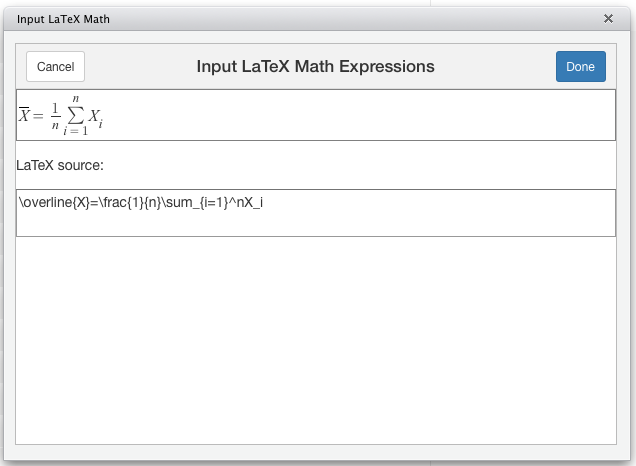
\includegraphics{images/mathquill} 

}

\caption{辅助输入 LaTeX 数学公式的 RStudio 插件}\label{fig:mathquill}
\end{figure}

还有其他 R 软件包提供了插件来帮助你编写书籍。\textbf{citr} 软件包 \citep{R-citr} 提供了一个名为``Insert citations''的加载项,可以很容易地将引用文献\index{citation}插入到 R Markdown 文档中。它会扫描你的文献数据库,并在下拉菜单中显示所有引用文献,因此你可以直接从列表中选择,而无需记住哪个引文键对应于哪个引文项(图 \ref{fig:citr})。

\begin{figure}

{\centering 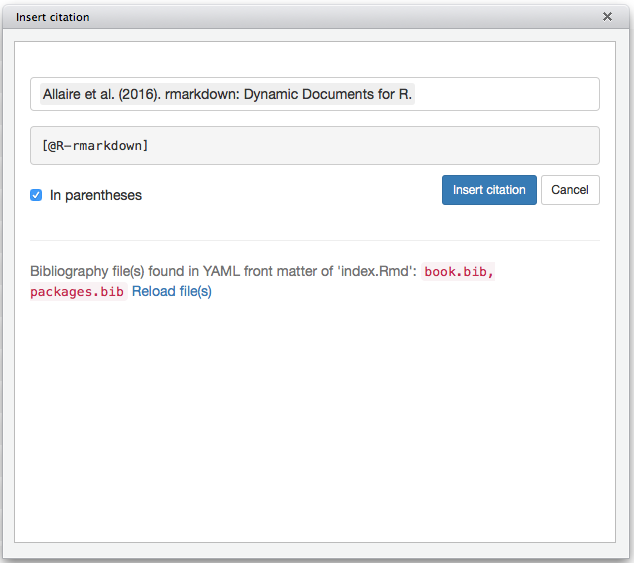
\includegraphics{images/citr} 

}

\caption{帮助插入引用文献的 RStudio 插件}\label{fig:citr}
\end{figure}

\section{协同工作}\label{collaboration}

今后创作书籍几乎肯定会涉及到多个人。你可能会和共同作者一起工作,以及不时提供反馈的读者。

由于所有书籍章节都是纯文本文件,因此它们非常适合用于应用版本控制工具。因此,如果你的所有合著者和合作者都具备 GIT 等版本控制工具的基本知识,你就可以使用这些工具与他们协作处理书籍内容。事实上,即使他们不知道如何使用 GIT,通过 GIT 进行协作也是可以的,因为 GitHub\index{GitHub}能够让使用者在 web 浏览器中在线创建和编辑文件。只需要有一个人必须熟悉 GIT,并且能够设置书籍存储库。其他合作者可以在线贡献内容,不过如果他们知道在本地使用 GIT 工作的基础用法,他们会有更多的自由。

读者可以通过两种方式做出贡献。一种方式是直接贡献内容,如果你的书源托管在 GitHub 上,最简单的方法是通过 \href{https://help.github.com/articles/about-pull-requests/}{GitHub pull requests}。基本上,任何 GitHub 用户都可以单击 Rmd 源文件页面上的编辑 (edit) 按钮,编辑内容,并将更改提交给你进行审批。如果你对提交的更改感到满意(你可以清楚地看到更改的内容),可以单击``合并 (Merge)''按钮来合并更改。如果你不满意,可以在 pull request 中提供反馈,以便读者根据要求进一步修改。我们在第 \ref{gitbook-style} 节中提到了 GitBook 样式中的编辑 (edit) 按钮。该按钮链接到每个页面的 Rmd 源文件,可以引导你创建 pull request。没有必要来回收发电子邮件来交流简单的更改内容,比如修改打字错误。

读者对你的书作出贡献的另一种方式是留下评论。评论可以以多种形式留下:电子邮件、GitHub issues 或 HTML 页面评论。这里我们使用 Disqus(参见第 \ref{yaml-options} 节)作为示例。Disqus 是一种在网页上嵌入讨论区的服务,可以通过 JavaScript 加载。当你注册并在 Disqus 上创建一个新的论坛后,你可以找到如下所示的 JavaScript 代码:

\begin{Shaded}
\begin{Highlighting}[]
\DataTypeTok{\textless{}}\KeywordTok{div}\OtherTok{ id}\OperatorTok{=}\StringTok{"disqus\_thread"}\DataTypeTok{\textgreater{}\textless{}/}\KeywordTok{div}\DataTypeTok{\textgreater{}}
\DataTypeTok{\textless{}}\KeywordTok{script}\DataTypeTok{\textgreater{}}
\NormalTok{(}\KeywordTok{function}\NormalTok{() \{ }\CommentTok{// DON\textquotesingle{}T EDIT BELOW THIS LINE}
\KeywordTok{var}\NormalTok{ d }\OperatorTok{=} \BuiltInTok{document}\OperatorTok{,}\NormalTok{ s }\OperatorTok{=}\NormalTok{ d}\OperatorTok{.}\FunctionTok{createElement}\NormalTok{(}\StringTok{\textquotesingle{}script\textquotesingle{}}\NormalTok{)}\OperatorTok{;}
\NormalTok{s}\OperatorTok{.}\AttributeTok{src} \OperatorTok{=} \StringTok{\textquotesingle{}//yihui.disqus.com/embed.js\textquotesingle{}}\OperatorTok{;}
\NormalTok{s}\OperatorTok{.}\FunctionTok{setAttribute}\NormalTok{(}\StringTok{\textquotesingle{}data{-}timestamp\textquotesingle{}}\OperatorTok{,} \OperatorTok{+}\KeywordTok{new} \BuiltInTok{Date}\NormalTok{())}\OperatorTok{;}
\NormalTok{(d}\OperatorTok{.}\AttributeTok{head} \OperatorTok{||}\NormalTok{ d}\OperatorTok{.}\AttributeTok{body}\NormalTok{)}\OperatorTok{.}\FunctionTok{appendChild}\NormalTok{(s)}\OperatorTok{;}
\NormalTok{\})()}\OperatorTok{;}
\DataTypeTok{\textless{}/}\KeywordTok{script}\DataTypeTok{\textgreater{}}
\DataTypeTok{\textless{}}\KeywordTok{noscript}\DataTypeTok{\textgreater{}}\NormalTok{Please enable JavaScript to view the}
\DataTypeTok{\textless{}}\KeywordTok{a}\OtherTok{ href}\OperatorTok{=}\StringTok{"https://disqus.com/?ref\_noscript"}\DataTypeTok{\textgreater{}}
\NormalTok{  comments powered by Disqus.}\DataTypeTok{\textless{}/}\KeywordTok{a}\DataTypeTok{\textgreater{}\textless{}/}\KeywordTok{noscript}\DataTypeTok{\textgreater{}}
\end{Highlighting}
\end{Shaded}

请注意,你需要用自己的论坛名称替换名称 \texttt{yihui}(创建新论坛时必须提供此名称)。你可以将代码保存到一个名为 \texttt{disqus.html} 的 HTML 文件中。然后可以通过 \texttt{after\_body} 选项将其嵌入到每页的末尾(图 \ref{fig:disqus} 显示了讨论区的外观):

\begin{Shaded}
\begin{Highlighting}[]
\PreprocessorTok{{-}{-}{-}}
\FunctionTok{output}\KeywordTok{:}
\AttributeTok{  bookdown:}\FunctionTok{:gitbook}\KeywordTok{:}
\AttributeTok{    }\FunctionTok{includes}\KeywordTok{:}
\AttributeTok{      }\FunctionTok{after\_body}\KeywordTok{:}\AttributeTok{ disqus.html}
\PreprocessorTok{{-}{-}{-}}
\end{Highlighting}
\end{Shaded}

\begin{figure}
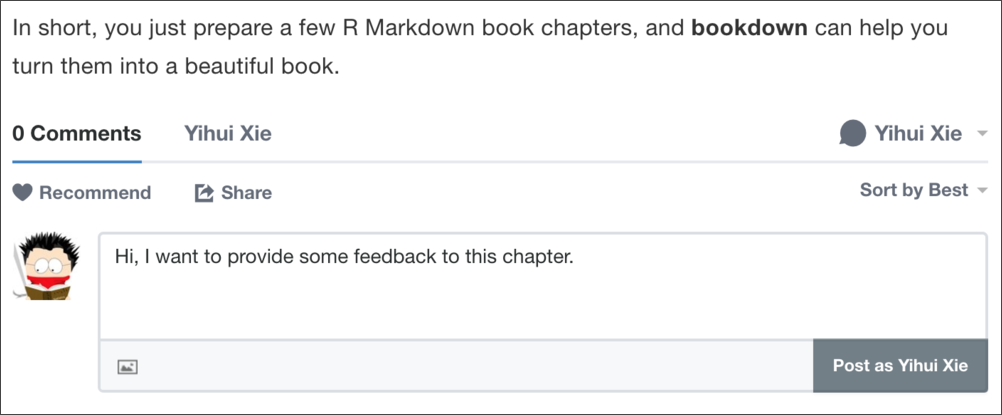
\includegraphics[width=1\linewidth]{images/disqus} \caption{有讨论区的书页。}\label{fig:disqus}
\end{figure}

\chapter{发布与出版}\label{publishing}

当你在创作书籍时,你可以将书稿提供给公众,例如,将书稿发布到网站上,以便从读者那里得到早期反馈。当你完成书籍的创作后,你需要考虑正式出版书籍的方式,可以通过印刷本也可以通过电子书进行出版。

\section{RStudio Connect}\label{rstudio-connect}

理论上,你可以自己编译书籍然后将其发布到你想要的任何地方。例如,你可以在自己的 Web 服务器上托管书籍的 HTML 版本。不过我们在 \textbf{bookdown} 中提供了一个函数 \texttt{publish\_book()} ,它能够让你很轻松地将书籍上传至 \url{https://bookdown.org}。这是一个由 RStudio 提供的网站,用于免费托管你的书籍。\index{bookdown.org}这个网站建立在 \href{https://posit.co/products/enterprise/connect/}{``RStudio Connect''}\index{RStudio Connect} 之上,它是 RStudio 提供的产品之一,能够让你将各种与 R 相关的应用部署到服务器上,包括 R Markdown 文档、Shiny 应用、R plots 等。

你不必了解太多 RStudio Connect 就能够将你的书籍发布到 bookdown.org。你需要在 \url{https://bookdown.org/connect/} 注册,之后当你第一次尝试运行 \texttt{bookdown::publish\_book()}\index{bookdown::publish\_book()} 时,系统将要求你授权 \textbf{bookdown} 发布到你的 bookdown.org 账户。以后使用时,只需要再次调用 \texttt{publish\_book()} 即可,\textbf{bookdown} 将不会要求你进行任何其他的操作。

\begin{Shaded}
\begin{Highlighting}[]
\FunctionTok{publish\_book}\NormalTok{(}\AttributeTok{name =} \ConstantTok{NULL}\NormalTok{, }\AttributeTok{account =} \ConstantTok{NULL}\NormalTok{,}
  \AttributeTok{server =} \ConstantTok{NULL}\NormalTok{, }\AttributeTok{render =} \FunctionTok{c}\NormalTok{(}\StringTok{"none"}\NormalTok{, }\StringTok{"local"}\NormalTok{, }\StringTok{"server"}\NormalTok{))}
\end{Highlighting}
\end{Shaded}

你需要接触的 \texttt{publish\_book()} 的唯一参数是 \texttt{render}。它决定了在发布之前是否编译书籍。如果你之前已经运行过 \texttt{render\_book()},就不需要改变这个参数,否则你可能需要将其设置为 \texttt{\textquotesingle{}local\textquotesingle{}}:

\begin{Shaded}
\begin{Highlighting}[]
\NormalTok{bookdown}\SpecialCharTok{::}\FunctionTok{publish\_book}\NormalTok{(}\AttributeTok{render =} \StringTok{\textquotesingle{}local\textquotesingle{}}\NormalTok{)}
\end{Highlighting}
\end{Shaded}

如果你已经配置好了自己的 RStudio Connect 服务器,那么当然可以将书籍发布到你自己的服务器,而不必上传至 bookdown.org。

\section{Netlify Drop}\label{netlify-drop}

Netlify (\url{https://netlify.com}) 是一个为静态网站提供云托管和无服务器后端服务的平台。Netlify 提供免费和付费两种服务,但他们也提供一种称为 Netlify Drop (\url{https://app.netlify.com/drop}) 的服务,这是一个免费的发布书籍的选项,并且不需要拥有 Netlify 帐户就能够使用。该服务不需要你的 \textbf{bookdown} 项目位于受版本控制的存储库中。你所需要的只是一个可以在本地构建的 \textbf{bookdown} 项目。

\subsection{构建和部署的工作流水线}\label{ux6784ux5efaux548cux90e8ux7f72ux7684ux5de5ux4f5cux6d41ux6c34ux7ebf}

这种发布方法设置了以下事件流:

\begin{enumerate}
\def\labelenumi{\arabic{enumi}.}
\tightlist
\item
  从本地 \textbf{bookdown} 项目开始。
\item
  在本地将书籍构建到所选的输出目录中(默认情况下为\texttt{\_book/})。
\item
  访问 Netlify Drop (\url{https://app.netlify.com/drop}),将输出目录拖放到 Netlify 基于浏览器的用户界面中。
\item
  对书籍进行修改,在本地重新构建,然后再次将输出目录拖放到 Netlify 中进行更新。
\end{enumerate}

以上内容仅为概述------请继续阅读以了解分步骤的说明。

\subsection{开始之前}\label{ux5f00ux59cbux4e4bux524d}

工作流水线从建立本地 \textbf{bookdown} 项目开始。项目并不需要放在 GitHub 或其它受版本控制的储存库内。

如果你没有线程的书籍,可以创建一个简单的 \textbf{bookdown} HTML 书籍来代替练习。有关如何在 RStudio 中创建新书的内容,请见图 \ref{fig:new-bs4-book};如果你不使用 RStudio,可以在 R console 中使用函数 \texttt{bookdown::create\_gitbook()} 或 \texttt{bookdown::create\_bs4\_book()}。

\subsection{构建书籍}\label{ux6784ux5efaux4e66ux7c4d}

在本地从你的 \textbf{bookdown} 项目中构建书籍,你可以使用第 \ref{build-the-book} 章中你喜欢的任何方法。

\subsection{部署网站}\label{ux90e8ux7f72ux7f51ux7ad9}

转到 Netlify Drop (\href{https://app.netlify.com/drop}{netlify.com/drop}),你应该能够在网页上看到一个方框,它高数你``将站点文件夹拖放到此处''。

接下来,将 \textbf{bookdown} 项目的输出目录(默认情况下为 \texttt{\_book/},除非你在 \texttt{\_bookdown.yml} 文件中更改了这项设置)拖放到 Web 浏览器中的这个方框中。你应该会看到你的书籍使用了 \texttt{https://random-word-12345.netlify.com} 形式的随机子域名进行快速部署。

你还会看到无人认领的网站会在 24 小时后被删除的通知。你可以注册一个 Netlify 账户来声明你的网站并使其永久在线。

\subsection{\texorpdfstring{\emph{可选:更新站点}}{可选:更新站点}}\label{ux53efux9009ux66f4ux65b0ux7ad9ux70b9}

注册 Netlify 后,你\emph{可以}更新这一类的网站,但它需要手动更新。访问 Netlify.com 并导航找到你的站点,然后单击``部署 (Deploys)''。你将看到一个方框,如图 \ref{fig:netlify-drag-drop} 所示,这表示你可以拖放站点文件夹以更新站点(你可能需要滚动到此页面底部)。

\begin{figure}

{\centering 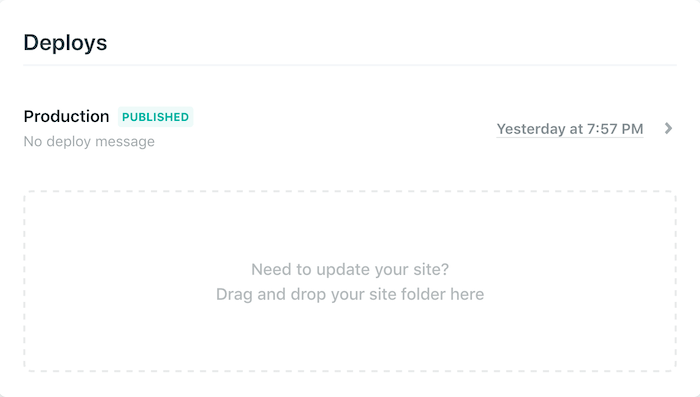
\includegraphics{images/netlify-drag-drop-update} 

}

\caption{在 Netlify 上拖放部署的站点更新方框的屏幕截图。}\label{fig:netlify-drag-drop}
\end{figure}

编辑你的书籍,再次在本地进行构建,然后将输出目录再次拖放到上传位置。

\subsection{\texorpdfstring{\emph{可选:更改默认子域名}}{可选:更改默认子域名}}\label{netlify-subdomain}

导航到 Netlify.com 上的站点登录页 (\url{https://app.netlify.com}),单击\emph{概述 (Overview) \textgreater{} 站点设置 (Site Settings)}。在\emph{站点信息 (Site information)}下单击\emph{更改站点名称 (Change site name)}并将其更新为你想要的名称。如果想使用自己的域名而不是 Netlify 的子域名,请阅读以下文档:\url{https://docs.netlify.com/domains-https/custom-domains/}。

\subsection{缺点和备选方案}\label{ux7f3aux70b9ux548cux5907ux9009ux65b9ux6848}

这个工作流非常适合快速共享书籍原型。但是,如果你选择不声明你的站点,该链接将在 24 小时后过期。即使你申请了网站并设置了 Netlify 帐户,这个工作流也不适合正在积极编辑或合作创作的书籍,因为每次更新书籍的本地版本时,你都需要手动将书籍上传到 Netlify。使用这种方法也无法获得版本控制的好处。

\section{GitHub}\label{github}

你可以使用 GitHub Pages (\url{https://pages.github.com}) 在 GitHub\index{GitHub} 上免费托管你的书籍。GitHub 支持 Jekyll (\url{http://jekyllrb.com}), 它是一个静态网站生成器,能够将一系列 Markdown 文件转换为网站。这可能是 GitHub Pages 最常见的用法,但是 GitHub 还支持任意静态 HTML 文件,因此你可以在 GitHub 上托管书籍的 HTML 输出文件。其关键是创建一个隐藏文件 \texttt{.nojekyll},它告诉 GitHub 你的网站不是通过 Jekyll 构建的,因为 \textbf{bookdown} 的 HTML 输出文件已经是一个独立的网站。

\begin{Shaded}
\begin{Highlighting}[]
\CommentTok{\# 假设你已经初始化了一个 git 储存库,并且已经在书籍储存库的目录下}

\CommentTok{\# 创建一个隐藏文件 .nojekyll}
\FunctionTok{touch}\NormalTok{ .nojekyll}
\CommentTok{\# 将其添加入 git 版本控制中,这样她就不会再 RStudio 中显示}
\FunctionTok{git}\NormalTok{ add .nojekyll}
\end{Highlighting}
\end{Shaded}

如果你使用 Windows,那么可能没有 \texttt{touch} 命令,这时你可以在 R 中使用 \texttt{file.create(\textquotesingle{}.nojekyll\textquotesingle{})} 来创建一个文件。

发布书籍的一种方法将书籍的 HTML 文件放入 \texttt{master} 分支中的 \texttt{/docs} 文件夹,然后从该文件夹将书籍作为 GitHub Pagse 站点发布,就像 \href{http://bit.ly/2cvloKV}{GitHub Help}中描述的那样。首先,在配置文件 \texttt{\_bookdown.yml} 中添加一行 \texttt{output\_dir:"docs"},将书籍的输出目录设置为 \texttt{/docs}。然后,将更改推送到 GitHub ,再转到存储库的设置,在``GitHub Pages''配置项下将``Source''选项更改为``master branch/docs folder''。使用该方法时,\texttt{.nojekyll} 文件必须位于 \texttt{/docs} 文件夹中。

另一种方法是先在存储库中创建一个 \texttt{gh-pages} 分支,再构建书籍,将 HTML 输出(包括图像、CSS 和 JavaScript 文件等所有外部资源)放入该分支,然后将该分支推送到远程存储库。如果你的书籍存储库没有 \texttt{gh-pages} 分支,可以使用以下命令创建一个分支:

\begin{Shaded}
\begin{Highlighting}[]
\CommentTok{\# 假设你已经初始化了一个 git 储存库,并且已经在书籍储存库的目录下}

\CommentTok{\# 创建一个名为 gh{-}pages 的分支,并清除全部文件}
\FunctionTok{git}\NormalTok{ checkout }\AttributeTok{{-}{-}orphan}\NormalTok{ gh{-}pages}
\FunctionTok{git}\NormalTok{ rm }\AttributeTok{{-}rf}\NormalTok{ .}

\CommentTok{\# 创建一个隐藏文件 .nojekyll}
\FunctionTok{touch}\NormalTok{ .nojekyll}
\FunctionTok{git}\NormalTok{ add .nojekyll}

\FunctionTok{git}\NormalTok{ commit }\AttributeTok{{-}m} \StringTok{"Initial commit"}
\FunctionTok{git}\NormalTok{ push origin gh{-}pages}
\end{Highlighting}
\end{Shaded}

设置好 GIT 之后,剩下的工作可以通过脚本(Shell、R 或 Makefile,取决于你的偏好)实现自动化。总的来说,首先将书籍编译为 HTML,然后运行 git 命令将文件推送到 GitHub,但你可能不希望在本地反复手动执行这些操作,这时可以通过云来完成。由于在云上实现发布过程的完全自动化将会非常方便,因此一旦设置正确,接下来所要做的就是编写书籍并将 Rmd 源文件推送到 GitHub,你创作的书将始终在服务器端自动构建和发布。

你可以选择使用的一个云服务是 Travis CI (\url{https://travis-ci.com})。\index{Travis CI} 它对于 GitHub 上的共有储存库提供的服务是免费的,并且是为软件包的持续集成 (CI) 而设计的。Travis CI 能够连接到 GitHub, 即每当你推送更改到 GitHub 时,Travis 能够被触发在最新版本的储存库上运行某些命令/脚本。\footnote{你需要先在 GitHub 上为你的储存库授权 Travis CI 服务。有关如何开始使用 Travis CI,请参阅 \url{https://docs.travis-ci.com/user/getting-started/}。}这些命令储存在你的储存库根目录下名为 \texttt{.travis.yml} 的 YAML 文件中。它们通常用于测试软件,但实际上它们的用途十分开放,这意味着你可以在 Travis(虚拟)机器上运行任意命令。也就是说,你当然可以在 Travis 上运行自己的脚本来构建书籍。注意,Travis 目前仅支持 Ubuntu 和 Mac OS X,因此你应该对于 Linux/Unix 命令有一些基本的了解。

下一个问题是,怎样将在 Travis 中构建的书籍发布到 GitHub?大体上说,你需要授予 Travis 对你的 GitHub 储存库的写访问权限。该授权能够通过集中方式完成,对于初学者来说最简单的方式是个人访问令牌 (personal access token)。以下是你可以遵循的几个操作步骤:

\begin{enumerate}
\def\labelenumi{\arabic{enumi}.}
\tightlist
\item
  对于你在 GitHub 上的账户创建一个 \href{http://bit.ly/2cEBYWB}{个人访问令牌 (personal access token)}(请确保启用``repo''作用域 (``repo'' scope),以便可以通过此令牌写入你的 GitHub 储存库)。
\item
  通过命令 \texttt{travis\ encrypt} 将其加密并放在环境变量 \texttt{GITHUB\_PAT} 里,然后储存在 \texttt{.travis.yml} 文件中。例如 \texttt{travis\ encrypt\ GITHUB\_PAT=TOKEN}。如果你不知道如何安装或使用 Travis 命令行工具,只需要将这个环境变量通过 \url{https://travis-ci.com/user/repo/settings} 储存起来,其中 \texttt{user} 是你的 GitHub ID,\texttt{repo} 是储存库的名称。
\item
  你可以使用你的 GitHub 令牌在 Travis 上克隆先前创建的这个 \texttt{gh-pages} 分支,向其添加从 R Markdown 转换而来的 HTML 输出文件(不要忘记添加图片和 CSS 样式文件),然后推送到远程储存库。
\end{enumerate}

假设你正在 \texttt{master} 分支中(你存放 Rmd 源文件的分支),并且已经编译好书籍,放在 \texttt{\_book} 目录中。接下来你可以在 Travis 中做的是:

\begin{Shaded}
\begin{Highlighting}[]
\CommentTok{\# 如果你还没有进行配置的话,设置好你的用户名和邮箱}
\FunctionTok{git}\NormalTok{ config }\AttributeTok{{-}{-}global}\NormalTok{ user.email }\StringTok{"you@example.com"}
\FunctionTok{git}\NormalTok{ config }\AttributeTok{{-}{-}global}\NormalTok{ user.name }\StringTok{"Your Name"}

\CommentTok{\# 将储存库克隆到书籍输出目录 book{-}output}
\FunctionTok{git}\NormalTok{ clone }\AttributeTok{{-}b}\NormalTok{ gh{-}pages }\DataTypeTok{\textbackslash{}}
\NormalTok{  https://}\VariableTok{$\{GITHUB\_PAT\}}\NormalTok{@github.com/}\VariableTok{$\{TRAVIS\_REPO\_SLUG\}}\NormalTok{.git }\DataTypeTok{\textbackslash{}}
\NormalTok{  book{-}output}
\BuiltInTok{cd}\NormalTok{ book{-}output}
\FunctionTok{git}\NormalTok{ rm }\AttributeTok{{-}rf} \PreprocessorTok{*}
\FunctionTok{cp} \AttributeTok{{-}r}\NormalTok{ ../\_book/}\PreprocessorTok{*}\NormalTok{ ./}
\FunctionTok{git}\NormalTok{ add }\AttributeTok{{-}{-}all} \PreprocessorTok{*}
\FunctionTok{git}\NormalTok{ commit }\AttributeTok{{-}m} \StringTok{"Update the book"}
\FunctionTok{git}\NormalTok{ push }\AttributeTok{{-}q}\NormalTok{ origin gh{-}pages}
\end{Highlighting}
\end{Shaded}

变量名 \texttt{GITHUB\_PAT} 和目录名 \texttt{book-output} 可以是任意名称。只要名称没有与已经存在的变量名或目录名冲突,你就可以使用喜欢的任何名字。上述脚本与我们在第 \ref{build-the-book} 节提到的书籍构建脚本可以放在 \texttt{master} 分支作为 as Shell 脚本。例如,你可以将它们命名为 \texttt{\_build.sh} 和 \texttt{\_deploy.sh}。那么,你的 \texttt{.travis.yml} 文件可能是这样的:

\begin{Shaded}
\begin{Highlighting}[]
\FunctionTok{language}\KeywordTok{:}\AttributeTok{ r}
\FunctionTok{pandoc\_version}\KeywordTok{:}\AttributeTok{ }\FloatTok{1.19.2.1}

\FunctionTok{env}\KeywordTok{:}
\AttributeTok{  }\FunctionTok{global}\KeywordTok{:}
\AttributeTok{    }\KeywordTok{{-}}\AttributeTok{ }\FunctionTok{secure}\KeywordTok{:}\AttributeTok{ A\_LONG\_ENCRYPTED\_STRING}

\FunctionTok{before\_script}\KeywordTok{:}
\AttributeTok{  }\KeywordTok{{-}}\AttributeTok{ chmod +x ./\_build.sh}
\AttributeTok{  }\KeywordTok{{-}}\AttributeTok{ chmod +x ./\_deploy.sh}

\FunctionTok{script}\KeywordTok{:}
\AttributeTok{  }\KeywordTok{{-}}\AttributeTok{ ./\_build.sh}
\AttributeTok{  }\KeywordTok{{-}}\AttributeTok{ ./\_deploy.sh}
\end{Highlighting}
\end{Shaded}

\texttt{language} 选项告诉 Travis 需要使用安装了 R 的虚拟机。\texttt{secure} 字段是加密的个人访问令牌 (personal access token )。如果你已经使用 Travis 上的 Web 界面而不是命令行工具 \texttt{travis\ encrypt} 保存了 \texttt{GITHUB\_PAT} 变量,则可以忽略这项设置。

由于 Travis 服务主要用于检查 R 软件包,因此还需要一个(假的)\texttt{DESCRIPTION} 文件,使得书籍存储库像是一个 R 软件包一样。这个文件中唯一一个真正重要的是软件包依赖项这一配置。所有依赖项都将通过 \textbf{devtools} 包安装。如果依赖项在 CRAN 或 BioConductor 上,只需在 \texttt{DESCRIPTION} 文件的 \texttt{Imports} 字段中列出即可。如果它在 GitHub 上,您可以使用 \texttt{Remotes} 字段列出它的存储库名称。下面展示了一个例子:

\begin{Shaded}
\begin{Highlighting}[]
\NormalTok{Package: placeholder}
\NormalTok{Type: Book}
\NormalTok{Title: Does not matter.}
\NormalTok{Version: 0.0.1}
\NormalTok{Imports: bookdown, ggplot2}
\NormalTok{Remotes: rstudio/bookdown}
\end{Highlighting}
\end{Shaded}

如果你使用 Travis 的 \href{https://docs.travis-ci.com/user/workers/container-based-infrastructure/}{container-based infrastructure},你可以在 \texttt{.travis.yml} 中使用 \texttt{sudo:\ false} 启用缓存。通常你至少需要缓存两类目录:图片目录(例如 \texttt{\_main\_files})以及缓存目录(例如 \texttt{\_main\_cache})。如果你指定了 \textbf{knitr} 代码块选项 \texttt{fig.path} 和 \texttt{cache.path},这些目录的名称可能不同,但是我强烈建议不要改变这些设置。图片和缓存目录都存放在书籍根目录中的 \texttt{\_bookdown\_files} 目录下。启用了 \textbf{knitr} 图片和缓存的 \texttt{.travis.yml} 文件可能具有如下的 \texttt{sudo} 和 \texttt{cache} 附加配置:

\begin{Shaded}
\begin{Highlighting}[]
\FunctionTok{sudo}\KeywordTok{:}\AttributeTok{ }\CharTok{false}

\FunctionTok{cache}\KeywordTok{:}
\AttributeTok{  }\FunctionTok{packages}\KeywordTok{:}\AttributeTok{ }\CharTok{yes}
\AttributeTok{  }\FunctionTok{directories}\KeywordTok{:}
\AttributeTok{    }\KeywordTok{{-}}\AttributeTok{ $TRAVIS\_BUILD\_DIR/\_bookdown\_files}
\end{Highlighting}
\end{Shaded}

如果构建书籍非常耗时,你可以在 Travis 上使用上面的配置来节省时间。注意,\texttt{packages:yes} 表示安装在 Travis 上的 R 包也被缓存。

以上所有脚本和配置都可以在 \texttt{bookdown-demo} 存储库中找到:\url{https://github.com/rstudio/bookdown-demo/}。如果你将它们复制到自己的存储库中,请记住使用自己的加密变量 \texttt{GITHUB\_PAT} 更改 \texttt{.travis.yml} 文件中的 \texttt{secure} 字段。

GitHub 和 Travis CI 当然不是构建和出版你的书籍的唯一选择。你可以在自己的服务器上自由地存储和发布这本书。

\section{HTML 发布功能}\label{html-ux53d1ux5e03ux529fux80fd}

\subsection{HTML 404 页面}\label{html-404}

如果读者试图访问书籍中无法找到的页面,浏览器将因为找不到请求的网页而显示 \href{https://en.wikipedia.org/wiki/HTTP_404}{404 错误}。这个 404 错误显示在一个 404 页面上。每个 web 服务器都有一个默认的 404 页面。但是大多数 web 服务平台,如 Netlify、Github Pages 和 Gitlab Pages 都会将网站根目录中名为 \texttt{404.html} 的文件用作自定义的错误提示网页(如果你能提供该文件)。

对于全部 HTML 书记格式,\textbf{bookdown} 会在你的输出目录中使用简单的内容(一个标题和 2 段正文)创建一个自定义的 \texttt{404.html};请见图 \ref{fig:404-page}。

\begin{figure}

{\centering 
\includegraphics{images/404} 

}

\caption{示例 404 页面的屏幕截图。}\label{fig:404-page}
\end{figure}

如您所见,这个 404 页面嵌入在书中,以便读者能够快速返回正在阅读的书籍内容。网页书籍站点的整体结构(包括导航栏、页脚、侧边栏等)和 CSS 样式仍然保留在 404 页面上。

要自定义 404 页面而不是使用 \textbf{bookdown} 提供的页面,你可以向项目根目录中添加 \texttt{\_404.Rmd} 或 \texttt{\_404.md} 文件。如果在编译书籍时找到前述任何一个文件,则该文件内容将被编译并作为嵌入书籍结构中的 404 页面的主体内容。

如果一个 404.html 文件已经存在于根目录级别的书籍源文档仓库中(与书籍的 \texttt{.Rmd} 文件放在一起),那么 \textbf{bookdown} 将保持该文件不变,并且不会将它覆盖。这是因为我们假设你的发布工作流中已经有了使用这个自定义的 \texttt{404.html} 的机制。

\subsection{用于共享的元数据}\label{metadata-for-sharing}

Bookdown HTML 书籍将使用你在 \texttt{index.Rmd} 的 YAML 中提供的信息,为 Twitter、Facebook 和 LinkedIn 等平台上的社交共享提供 HTML 元数据。要对其进行设置,请设置书籍的 \texttt{url} 和 \texttt{cover-image} 文件的路径。该路径可以是绝对 URL,也可以是项目中图像文件的相对路径。书籍的 \texttt{title} 和 \texttt{description} 也会被使用。设置这些选项能带来一个很好的效果,当读者在社交网络网站上共享你的书籍的链接时,该链接将自动扩展为带有书籍封面图像和描述的卡片。

\begin{figure}

\includegraphics[width=0.4755\linewidth]{images/social-og} 
\includegraphics[width=0.5145\linewidth]{images/social-twitter} \caption{当链接在 Facebook 和 LinkedIn(左侧)和 Twitter(右侧)上被共享时,显示 HTML 书籍封面图像、标题和描述的屏幕截图。}\label{fig:social}
\end{figure}

无论使用哪种方法发布 HTML 书籍,都可以使用 \url{https://www.opengraph.xyz} 来检查书籍元数据,它显示了跨平台共享链接时链接外观的预览。你还可以使用特定于平台的开发人员工具:

\begin{itemize}
\tightlist
\item
  Facebook: \url{https://developers.facebook.com/tools/debug/}
\item
  LinkedIn: \url{https://www.linkedin.com/post-inspector/}
\item
  Twitter: \url{https://cards-dev.twitter.com/validator}
\end{itemize}

\section{出版商}\label{ux51faux7248ux5546}

除了在网上发布你的书之外,你还可以考虑通过出版商\index{publisher}出版你的书籍。例如,本书是由 Chapman \& Hall/CRC 出版的,在 \url{https://bookdown.org/yihui/bookdown/} 也有免费的在线版本(与出版商达成了协议)。如果你不想与的发布者合作,你还可以考虑自主出版 (\url{https://en.wikipedia.org/wiki/Self-publishing})。Pablo Casas 写了两篇你可能会觉得有用的博客文章:\href{https://blog.datascienceheroes.com/how-to-self-publish-a-book/}{``How to self-publish a book''} 和 \href{https://blog.datascienceheroes.com/how-to-self-publish-a-book-customizing-bookdown/}{``How to self-publish a book: customizing bookdown''}。

如果你选择的出版商支持 LaTeX,那么出版用 \textbf{bookdown} 编写的书会容易得多。\index{LaTeX}例如,Chapman \& Hall 提供了一个名为 \texttt{krantz.cls} 的 LaTeX 类,Springer 提供的是 \texttt{svmono.cls}。如果要将这些 LaTeX 类应用于 PDF 书籍,请将 \texttt{index.Rmd} 的 YAML 元数据中的 \texttt{documentclass} 设置为 LaTeX 类文件名(不带扩展名 \texttt{.cls})。

LaTeX 类是 YAML 元数据中最重要的设置。它控制了 PDF 书籍的整体样式。还有一些其他设置是你经常需要调整的,下面我们将展示有关本书的一些详细信息。

本书的 YAML 元数据包含以下设置:

\begin{Shaded}
\begin{Highlighting}[]
\FunctionTok{documentclass}\KeywordTok{:}\AttributeTok{ krantz}
\FunctionTok{lot}\KeywordTok{:}\AttributeTok{ }\CharTok{yes}
\FunctionTok{lof}\KeywordTok{:}\AttributeTok{ }\CharTok{yes}
\FunctionTok{fontsize}\KeywordTok{:}\AttributeTok{ 12pt}
\FunctionTok{monofont}\KeywordTok{:}\AttributeTok{ }\StringTok{"Source Code Pro"}
\FunctionTok{monofontoptions}\KeywordTok{:}\AttributeTok{ }\StringTok{"Scale=0.7"}
\end{Highlighting}
\end{Shaded}

字段 \texttt{lot:yes} 表示我们需要表格列表;类似地,\texttt{lof} 表示图片列表。基础字体大小是 `12pt',我们使用了 \href{https://www.fontsquirrel.com/fonts/source-code-pro}{Source Code Pro} 作为等宽(固定宽度)字体,它适用于本书中的所有程序代码。

在 LaTeX 导言 (preamble)(第 \ref{yaml-options} 节)中,我们还有一些设置。首先,我们将主字体族\index{font}设置为 \href{https://www.fontsquirrel.com/fonts/alegreya}{Alegreya},并且由于此字体没有 {Small Capitals}(小型大写字母)特征,我们使用 Alegreya SC 字体。

\begin{Shaded}
\begin{Highlighting}[]
\FunctionTok{\textbackslash{}setmainfont}\NormalTok{[}
\NormalTok{  UprightFeatures=\{SmallCapsFont=AlegreyaSC{-}Regular\}}
\NormalTok{]\{Alegreya\}}
\end{Highlighting}
\end{Shaded}

下面的命令通过允许浮动环境\index{floating environment}占用更大部分的页面而不是浮动,从而使得它们更不太可能浮动。

\begin{Shaded}
\begin{Highlighting}[]
\FunctionTok{\textbackslash{}renewcommand}\NormalTok{\{}\ExtensionTok{\textbackslash{}textfraction}\NormalTok{\}\{0.05\}}
\FunctionTok{\textbackslash{}renewcommand}\NormalTok{\{}\ExtensionTok{\textbackslash{}topfraction}\NormalTok{\}\{0.8\}}
\FunctionTok{\textbackslash{}renewcommand}\NormalTok{\{}\ExtensionTok{\textbackslash{}bottomfraction}\NormalTok{\}\{0.8\}}
\FunctionTok{\textbackslash{}renewcommand}\NormalTok{\{}\ExtensionTok{\textbackslash{}floatpagefraction}\NormalTok{\}\{0.75\}}
\end{Highlighting}
\end{Shaded}

由于 \texttt{krantz.cls} 为引用文段提供了一个环境 \texttt{VF},因此我们将标准的 \texttt{quote} 环境重新定义为 \texttt{VF}。您可以在第 \ref{markdown-syntax} 节中看到它的样式。

\begin{Shaded}
\begin{Highlighting}[]
\FunctionTok{\textbackslash{}renewenvironment}\NormalTok{\{quote\}\{}\KeywordTok{\textbackslash{}begin}\NormalTok{\{}\ExtensionTok{VF}\NormalTok{\}\}\{}\KeywordTok{\textbackslash{}end}\NormalTok{\{}\ExtensionTok{VF}\NormalTok{\}\}}
\end{Highlighting}
\end{Shaded}

然后我们将超链接重新定义为脚注,因为当书印刷在纸上时,读者无法点击文本中的链接,而脚注会告诉他们实际的链接是什么。

\begin{Shaded}
\begin{Highlighting}[]
\FunctionTok{\textbackslash{}let\textbackslash{}oldhref\textbackslash{}href}
\FunctionTok{\textbackslash{}renewcommand}\NormalTok{\{}\ExtensionTok{\textbackslash{}href}\NormalTok{\}[2]\{\#2}\FunctionTok{\textbackslash{}footnote}\NormalTok{\{}\FunctionTok{\textbackslash{}url}\NormalTok{\{\#1\}\}\}}
\end{Highlighting}
\end{Shaded}

我们还为 \texttt{\_output.yml}\index{\_output.yml} 中的 \texttt{bookdown::pdf\_book} 格式进行了一些设置:

\begin{Shaded}
\begin{Highlighting}[]
\AttributeTok{bookdown:}\FunctionTok{:pdf\_book}\KeywordTok{:}
\AttributeTok{  }\FunctionTok{includes}\KeywordTok{:}
\AttributeTok{    }\FunctionTok{in\_header}\KeywordTok{:}\AttributeTok{ latex/preamble.tex}
\AttributeTok{    }\FunctionTok{before\_body}\KeywordTok{:}\AttributeTok{ latex/before\_body.tex}
\AttributeTok{    }\FunctionTok{after\_body}\KeywordTok{:}\AttributeTok{ latex/after\_body.tex}
\AttributeTok{  }\FunctionTok{keep\_tex}\KeywordTok{:}\AttributeTok{ }\CharTok{yes}
\AttributeTok{  }\FunctionTok{dev}\KeywordTok{:}\AttributeTok{ }\StringTok{"cairo\_pdf"}
\AttributeTok{  }\FunctionTok{latex\_engine}\KeywordTok{:}\AttributeTok{ xelatex}
\AttributeTok{  }\FunctionTok{citation\_package}\KeywordTok{:}\AttributeTok{ natbib}
\AttributeTok{  }\FunctionTok{template}\KeywordTok{:}\AttributeTok{ }\CharTok{null}
\AttributeTok{  }\FunctionTok{pandoc\_args}\KeywordTok{:}\AttributeTok{ {-}{-}top{-}level{-}division=chapter}
\AttributeTok{  }\FunctionTok{toc\_unnumbered}\KeywordTok{:}\AttributeTok{ }\CharTok{no}
\AttributeTok{  }\FunctionTok{toc\_appendix}\KeywordTok{:}\AttributeTok{ }\CharTok{yes}
\AttributeTok{  }\FunctionTok{quote\_footer}\KeywordTok{:}\AttributeTok{ }\KeywordTok{[}\StringTok{"}\SpecialCharTok{\textbackslash{}\textbackslash{}}\StringTok{VA\{"}\KeywordTok{,}\AttributeTok{ }\StringTok{"\}\{\}"}\KeywordTok{]}
\AttributeTok{  }\FunctionTok{highlight\_bw}\KeywordTok{:}\AttributeTok{ }\CharTok{yes}
\end{Highlighting}
\end{Shaded}

我们上面提到的所有导言 (preamble) 设置都在文件 \texttt{latex/preamble.tex} 中,其中我们还指定了前言 (front matter) 的开始:

\begin{quote}
译者注:\texttt{\textbackslash{}frontmatter} 通常跟在 \texttt{\textbackslash{}begin\{document\}} 后,会关闭章节序号,页码使用罗马数字。
\end{quote}

\begin{Shaded}
\begin{Highlighting}[]
\FunctionTok{\textbackslash{}frontmatter}
\end{Highlighting}
\end{Shaded}

在 \texttt{latex/before\_body.tex} 中,我们插入了出版商要求的一些空白页,并编写了奉献页。在书的第一章之前,我们插入

\begin{Shaded}
\begin{Highlighting}[]
\FunctionTok{\textbackslash{}mainmatter}
\end{Highlighting}
\end{Shaded}

因此,LaTeX 知道将页码样式从罗马数字(前言所用的样式)更改为阿拉伯数字(正文所用的样式)。

我们在 \texttt{latex/after\_body.tex}(第 \ref{latex-index} 节)中打印索引。

由于默认设备 \texttt{pdf} 不能嵌入字体,因此用于保存图片的图形设备 (\texttt{dev}) 被设置为 \texttt{cairo\_pdf},以便字体可以嵌入图片中。你的文案编辑可能会要求您嵌入 PDF 中使用的所有字体,以便该书可以完全按其电子版本的外观打印,否则某些字体可能会被替换,印刷时的字型可能无法预测。

\texttt{quote\_footer} 字段是为了确保引用页脚右对齐:\texttt{krantz.cls} 提供了 LaTeX 命令 \texttt{\textbackslash{}VA\{\}} 以包含引用页脚。

\texttt{highlight\_bw} 选项被设置为 true,这样语法高亮显示的代码块中的颜色将转换为灰度,因为这本书将采用黑白打印。

这本书是通过 \texttt{xelatex} 编译成 PDF 的,以便于我们使用自定义字体。

除 \texttt{VF} 环境和 \texttt{\textbackslash{}VA\{\}} 命令外,上述所有设置都可以应用于任何其他 LaTeX 文档类。

如果你也想与 Chapman \& Hall 合作,你可以从我们存储库 (\url{https://github.com/rstudio/bookdown/tree/master/inst/examples}) 中的 \texttt{krantz.cls} 文件开始,而不使用你从编辑那里得到的副本。我们已经与 LaTeX 帮助中心合作解决了这个 LaTeX 类的许多问题,所以如果你使用 \textbf{bookdown},希望它能很好地用于你的书。

\cleardoublepage

\appendix \addcontentsline{toc}{chapter}{\appendixname}


\chapter{软件工具}\label{software-tools}

对于不熟悉如何使用 R Markdown 的依赖软件包的人,我们将简要介绍这些软件包的安装和维护。

\section{R 和 R 软件包}\label{r-ux548c-r-ux8f6fux4ef6ux5305}

你能够从任何一个 CRAN (the Comprehensive R Archive Network) 镜像站中下载并安装 R,例如 \url{https://cran.rstudio.com}。请注意每年都会有一些 R 的新版本发布,你可能需要偶尔进行升级。

为了安装 \textbf{bookdown} 包,你可以在 R 中输入:

\begin{Shaded}
\begin{Highlighting}[]
\FunctionTok{install.packages}\NormalTok{(}\StringTok{"bookdown"}\NormalTok{)}
\end{Highlighting}
\end{Shaded}

这将安装所有必需的 R 包。如果你不太关心这些包是否真的会被用来编译你的书籍(例如 \textbf{htmlwidgets}),也可以选择安装所有可选的包:

\begin{Shaded}
\begin{Highlighting}[]
\FunctionTok{install.packages}\NormalTok{(}\StringTok{"bookdown"}\NormalTok{, }\AttributeTok{dependencies =} \ConstantTok{TRUE}\NormalTok{)}
\end{Highlighting}
\end{Shaded}

如果你想体验 GitHub 上 \textbf{bookdown} 的开发版本,需要首先安装 \textbf{devtools}:

\begin{Shaded}
\begin{Highlighting}[]
\ControlFlowTok{if}\NormalTok{ (}\SpecialCharTok{!}\FunctionTok{requireNamespace}\NormalTok{(}\StringTok{\textquotesingle{}devtools\textquotesingle{}}\NormalTok{)) }\FunctionTok{install.packages}\NormalTok{(}\StringTok{\textquotesingle{}devtools\textquotesingle{}}\NormalTok{)}
\NormalTok{devtools}\SpecialCharTok{::}\FunctionTok{install\_github}\NormalTok{(}\StringTok{\textquotesingle{}rstudio/bookdown\textquotesingle{}}\NormalTok{)}
\end{Highlighting}
\end{Shaded}

R 包也经常在 CRAN 或 GitHub 上不断更新,所以你可能需要偶尔更新它们:

\begin{Shaded}
\begin{Highlighting}[]
\FunctionTok{update.packages}\NormalTok{(}\AttributeTok{ask =} \ConstantTok{FALSE}\NormalTok{)}
\end{Highlighting}
\end{Shaded}

尽管不是必需的,但当你从事与 R 相关的项目时,使用 RStudio IDE 能够使很多事情变得更加简单。你可以从 \url{https://www.posit.co} 下载 RStudio IDE。

\section{Pandoc}\label{pandoc}

R Markdown 文档 (\texttt{*.Rmd}) 首先会通过 \textbf{knitr} 包编译成 Markdown (\texttt{*.md}),然后 Markdown 再通过 Pandoc 编译成其他输出格式(如 LaTeX 或 HTML)。\index{Pandoc}整个过程是由 \textbf{rmarkdown} 包自动完成的。你不需要额外安装 \textbf{knitr} 或 \textbf{rmarkdown},因为它们是 \textbf{bookdown} 的依赖包,在安装 \textbf{bookdown} 时会自动安装。然而,Pandoc 并不是 R 软件包,因此不会在安装 \textbf{bookdown} 时自动安装。你可以参考 Pandoc 主页 (\url{http://pandoc.org}) 上的安装说明来安装 Pandoc,但如果你使用 RStudio IDE,则不需要额外安装 Pandoc,因为 RStudio 已经包含了一个 Pandoc 的副本。你可以通过以下方式查看 Pandoc 版本号:

\begin{Shaded}
\begin{Highlighting}[]
\NormalTok{rmarkdown}\SpecialCharTok{::}\FunctionTok{pandoc\_version}\NormalTok{()}
\DocumentationTok{\#\# [1] \textquotesingle{}3.2\textquotesingle{}}
\end{Highlighting}
\end{Shaded}

如果你发现这个版本太低了,并且一些 Pandoc 功能特性只在更高版本中提供,你可以安装更高版本的 Pandoc,之后 \textbf{rmarkdown} 将会调用更高版本的 Pandoc,而不是内置的版本。

\section{LaTeX}\label{latex}

只有当你想要将书籍输出为 PDF 时,你才需要 LaTeX\index{LaTeX}。你可以通过访问 \url{https://www.latex-project.org/get/} 来获取更多关于 LaTeX 及其安装的信息,但是我们强烈推荐你安装名为 \href{https://yihui.org/tinytex/}{TinyTeX} 的轻量级跨平台 LaTeX 发行版,它是基于 TeX Live 构建的。TinyTeX 能够通过 R 包 \textbf{tinytex} 轻松安装(安装 \textbf{bookdown} 时将自动安装):

\begin{Shaded}
\begin{Highlighting}[]
\NormalTok{tinytex}\SpecialCharTok{::}\FunctionTok{install\_tinytex}\NormalTok{()}
\end{Highlighting}
\end{Shaded}

使用 TinyTeX,你应该永远不会看见这样的错误信息:

\begin{Shaded}
\begin{Highlighting}[]
\NormalTok{! LaTeX Error: File \textasciigrave{}titling.sty\textquotesingle{} not found.}

\NormalTok{Type X to quit or \textless{}RETURN\textgreater{} to proceed,}
\NormalTok{or enter new name. (Default extension: sty)}

\NormalTok{Enter file name: }
\NormalTok{! Emergency stop.}
\NormalTok{\textless{}read *\textgreater{} }
         
\NormalTok{l.107 \^{}\^{}M}

\NormalTok{pandoc: Error producing PDF}
\NormalTok{Error: pandoc document conversion failed with error 43}
\NormalTok{Execution halted}
\end{Highlighting}
\end{Shaded}

上面的错误信息表示你使用了一个包含 \texttt{titling.sty} 文件的 LaTeX 包,但并没有安装该软件包。LaTeX 包名通常是 \texttt{*.sty} 的格式,因此在本例中,你可以尝试安装 \texttt{titling} 包。如果你在 R Markdown 中使用 TinyTeX,缺少的 LaTeX 包将会自动安装,因此无需担心此类问题。

LaTeX 发行版和其软件包也会不时进行更新,你可以考虑更新它们,特别是当遇到 LaTeX 问题时。你可以通过以下方式查看 LaTeX 发行版的版本:

\begin{Shaded}
\begin{Highlighting}[]
\FunctionTok{system}\NormalTok{(}\StringTok{\textquotesingle{}pdflatex {-}{-}version\textquotesingle{}}\NormalTok{)}
\DocumentationTok{\#\#  pdfTeX 3.141592653{-}2.6{-}1.40.26 (TeX Live 2024)}
\DocumentationTok{\#\#  kpathsea version 6.4.0}
\DocumentationTok{\#\#  Copyright 2024 Han The Thanh (pdfTeX) et al.}
\DocumentationTok{\#\#  There is NO warranty.  Redistribution of this software is}
\DocumentationTok{\#\#  covered by the terms of both the pdfTeX copyright and}
\DocumentationTok{\#\#  the Lesser GNU General Public License.}
\DocumentationTok{\#\#  For more information about these matters, see the file}
\DocumentationTok{\#\#  named COPYING and the pdfTeX source.}
\DocumentationTok{\#\#  Primary author of pdfTeX: Han The Thanh (pdfTeX) et al.}
\DocumentationTok{\#\#  Compiled with libpng 1.6.43; using libpng 1.6.43}
\DocumentationTok{\#\#  Compiled with zlib 1.3.1; using zlib 1.3.1}
\DocumentationTok{\#\#  Compiled with xpdf version 4.04}
\end{Highlighting}
\end{Shaded}

你可以运行以下代码来更新 TinyTeX:

\begin{Shaded}
\begin{Highlighting}[]
\NormalTok{tinytex}\SpecialCharTok{::}\FunctionTok{tlmgr\_update}\NormalTok{()}
\end{Highlighting}
\end{Shaded}

随着时间的推移,你可能也需要升级 TinyTeX(否则你无法安装或更新任何 LaTeX 软件包),在这种情况下你需要重新安装 TinyTeX:

\begin{Shaded}
\begin{Highlighting}[]
\NormalTok{tinytex}\SpecialCharTok{::}\FunctionTok{reinstall\_tinytex}\NormalTok{()}
\end{Highlighting}
\end{Shaded}

\chapter{软件使用}\label{software-usage}

如第 \ref{introduction} 章所述,这本书并不是一本全面的 \textbf{knitr} 或 \textbf{rmarkdown} 指南。在本章中,我们简要地解释了 \textbf{knitr} 和 \textbf{rmarkdown} 中的一些基本概念和语法。如果你有更多的问题,可以在 StackOverflow (\url{https://stackoverflow.com}) 上提问,并用 \texttt{r}、\texttt{knitr}、\texttt{rmarkdown} 和/或 \texttt{bookdown} 等任何适合的标签标记你的问题。

\section{knitr}\label{knitr}

\textbf{knitr} 包\index{knitr}是基于``文学化编程 (Literate Programming)''\citep{knuth1984}的思想设计的,它允许你在源文档中将程序代码与文本混合在一起。当 \textbf{knitr} 编译文档时,程序代码(以代码块为单位)会被提取并执行,程序输出将与原始文本一起展示在输出文档中。我们在第 \ref{r-code} 节中介绍了基本的语法。

R Markdown 不是 \textbf{knitr} 支持的唯一源格式。\textbf{knitr} 的基本思想可应用于其他计算和创作语言。例如,\textbf{knitr}还支持 R 和 LaTeX 的组合(\texttt{*.rnw}文档),以及 R + HTML (\texttt{*.RtML}) 等。你也可以在 \textbf{knitr} 中 使用其他计算语言,如 C++、Python、SQL 等。下面是一个简单的例子,你可以在 \url{http://rmarkdown.rstudio.com/authoring_knitr_engines.html} 中了解更多信息。

\begin{Shaded}
\begin{Highlighting}[]
\InformationTok{\textasciigrave{}\textasciigrave{}\textasciigrave{}\{python\}}
\InformationTok{x = \textquotesingle{}Hello, Python World!\textquotesingle{}}
\InformationTok{print(x.split(\textquotesingle{} \textquotesingle{}))}
\InformationTok{\textasciigrave{}\textasciigrave{}\textasciigrave{}}
\end{Highlighting}
\end{Shaded}

Python 用户可能熟悉 IPython\index{IPython} 或 Jupyter\index{Jupyter Notebook} Notebooks (\url{https://jupyter.org})。事实上,R Markdown 也可以作为笔记本使用,并有一些额外的优势;有关这方面详细信息,请参阅这篇博客文章:\url{https://blog.rstudio.org/2016/10/05/r-notebooks/}。

如果要在文档中显示文本形式的代码块,可以在块头部之前添加一个内联表达式,该表达式生成一个空字符串 (\texttt{\textasciigrave{}r\ \textquotesingle{}\textquotesingle{}\textasciigrave{}}),并将代码块用在四个反引号包裹起来,\footnote{如果要在列表等其他环境中显示文字形式的代码块,请遵循缩进规则:\url{https://pandoc.org/MANUAL.html\#block-content-in-list-items}}例如:

\begin{Shaded}
\begin{Highlighting}[]
\InformationTok{\textasciigrave{}\textasciigrave{}\textasciigrave{}\textasciigrave{}}
\InformationTok{\textasciigrave{}r \textquotesingle{}\textquotesingle{}\textasciigrave{}\textasciigrave{}\textasciigrave{}\textasciigrave{}\{r\}}
\InformationTok{\# a literal code chunk}
\InformationTok{\textasciigrave{}\textasciigrave{}\textasciigrave{}}
\InformationTok{\textasciigrave{}\textasciigrave{}\textasciigrave{}\textasciigrave{}}
\end{Highlighting}
\end{Shaded}

当文档被编译后,内联表达式将会消失,你会看到:

\begin{Shaded}
\begin{Highlighting}[]
\InformationTok{\textasciigrave{}\textasciigrave{}\textasciigrave{}\{r\}}
\InformationTok{\# a literal code chunk}
\InformationTok{\textasciigrave{}\textasciigrave{}\textasciigrave{}}
\end{Highlighting}
\end{Shaded}

编译文档时通常不需要直接调用 \textbf{knitr} 函数,因为 \textbf{rmarkdown} 会调用 \textbf{knitr}。如果你希望编译源文档而不进一步将其转换为其他格式,可以使用 \texttt{knitr::knit()} 函数。

\section{R Markdown}\label{r-markdown}

得益于 R 和 Pandoc 的强大功能,你可以轻松地在 R Markdown 文档中进行计算,并将其转换为各种输出格式,包括 HTML/PDF/Word 文档、HTML5/Beamer 幻灯片、仪表板和网站等。一份 R Markdown 文档通常由 YAML\index{YAML} 元数据(可选)和文档主体组成。我们在第 \ref{components} 章中介绍了编写文档主体各个组件的语法,并将在本节详细解释 YAML 元数据。

R Markdown 的元数据可以写在文档的最开头,分别以三个短划线 \texttt{-\/-\/-} 开头和结尾。YAML 元数据通常由冒号分隔的标签和值组成,例如:

\begin{Shaded}
\begin{Highlighting}[]
\PreprocessorTok{{-}{-}{-}}
\FunctionTok{title}\KeywordTok{:}\AttributeTok{ }\StringTok{"An R Markdown Document"}
\FunctionTok{author}\KeywordTok{:}\AttributeTok{ }\StringTok{"Yihui Xie"}
\PreprocessorTok{{-}{-}{-}}
\end{Highlighting}
\end{Shaded}

对于字符类型的取值,当不包含特殊字符时,你可以省略引号,但如果希望它们被解析为字符类型,则使用引号更为安全。

除字符类型外,另一种常见类型是逻辑类型。\texttt{yes} 和 \texttt{true} 都表示 true,\texttt{no}/\texttt{false} 都表示 false,例如:

\begin{Shaded}
\begin{Highlighting}[]
\FunctionTok{link{-}citations}\KeywordTok{:}\AttributeTok{ }\CharTok{yes}
\end{Highlighting}
\end{Shaded}

元数据取值也可以是向量,并且有两种写入向量的方法。下面列出的两种方法是等价的

\begin{Shaded}
\begin{Highlighting}[]
\FunctionTok{output}\KeywordTok{:}\AttributeTok{ }\KeywordTok{[}\StringTok{"html\_document"}\KeywordTok{,}\AttributeTok{ }\StringTok{"word\_document"}\KeywordTok{]}
\end{Highlighting}
\end{Shaded}

\begin{Shaded}
\begin{Highlighting}[]
\FunctionTok{output}\KeywordTok{:}
\AttributeTok{  }\KeywordTok{{-}}\AttributeTok{ }\StringTok{"html\_document"}
\AttributeTok{  }\KeywordTok{{-}}\AttributeTok{ }\StringTok{"word\_document"}
\end{Highlighting}
\end{Shaded}

元数据取值也可以是键值对的列表,只需要将其额外缩进两个空格,例如:

\begin{Shaded}
\begin{Highlighting}[]
\FunctionTok{output}\KeywordTok{:}
\AttributeTok{  bookdown:}\FunctionTok{:gitbook}\KeywordTok{:}
\AttributeTok{    }\FunctionTok{split\_by}\KeywordTok{:}\AttributeTok{ }\StringTok{"section"}
\AttributeTok{    }\FunctionTok{split\_bib}\KeywordTok{:}\AttributeTok{ }\CharTok{no}
\end{Highlighting}
\end{Shaded}

忘记缩进是一个常见的错误。例如,下面的数据

\begin{Shaded}
\begin{Highlighting}[]
\FunctionTok{output}\KeywordTok{:}
\FunctionTok{html\_document}\KeywordTok{:}
\FunctionTok{toc}\KeywordTok{:}\AttributeTok{ }\CharTok{yes}
\end{Highlighting}
\end{Shaded}

实际上表示

\begin{Shaded}
\begin{Highlighting}[]
\FunctionTok{output}\KeywordTok{:}\AttributeTok{ }\CharTok{null}
\FunctionTok{html\_document}\KeywordTok{:}\AttributeTok{ }\CharTok{null}
\FunctionTok{toc}\KeywordTok{:}\AttributeTok{ }\CharTok{yes}
\end{Highlighting}
\end{Shaded}

而不是你期望的那样:

\begin{Shaded}
\begin{Highlighting}[]
\FunctionTok{output}\KeywordTok{:}
\AttributeTok{  }\FunctionTok{html\_document}\KeywordTok{:}
\AttributeTok{    }\FunctionTok{toc}\KeywordTok{:}\AttributeTok{ }\CharTok{yes}
\end{Highlighting}
\end{Shaded}

R Markdown 输出格式是在 YAML 元数据的 \texttt{output} 字段中指定的,你需要查阅 R 帮助页面以获得可以填写的选项,例如 \texttt{?rmarkdown::html\_document} 或 \texttt{?bookdown::gitbook}。YAML 中其它大多数字段的含义可以在 Pandoc 文档中找到。

\textbf{rmarkdown} 软件包提供了这些 R Markdown 输出格式:

\begin{itemize}
\tightlist
\item
  \texttt{beamer\_presentation}
\item
  \texttt{context\_document}
\item
  \texttt{github\_document}
\item
  \texttt{html\_document}
\item
  \texttt{ioslides\_presentation}
\item
  \texttt{latex\_document}
\item
  \texttt{md\_document}
\item
  \texttt{odt\_document}
\item
  \texttt{pdf\_document}
\item
  \texttt{powerpoint\_presentation}
\item
  \texttt{rtf\_document}
\item
  \texttt{slidy\_presentation}
\item
  \texttt{word\_document}
\end{itemize}

在其他 R 包中还支持了更多的输出格式,包括 \textbf{bookdown}、\textbf{tufte}、\textbf{rticles}、\textbf{flexdashboard}、\textbf{revealjs} 和 \textbf{rmdformats}等。

\chapter{常见问题}\label{ux5e38ux89c1ux95eeux9898}

下面是\emph{完整的}常见问题 (FAQ) 列表。是的,这里只有一个问题。我个人不喜欢 FAQs。它们通常意味着意料之外的事物,而这对软件用户来说并不友好。

\begin{enumerate}
\def\labelenumi{\arabic{enumi}.}
\item
  问:\textbf{bookdown} 会不会有 X、Y 和 Z功能?

  答:简而言之,答案是否定的。但是如果你已经多次询问自己``我真的需要这些功能吗'',而答案仍然是``是''时,请随时向我们提出功能要求 \url{https://github.com/rstudio/bookdown/issues}。

  需要更多功能的用户往往来自 LaTeX 世界。如果你是这种情况,这个问题的答案是肯定的,因为 Pandoc 的 Markdown 支持原始 LaTeX 代码。每当你觉得 Markdown 不能帮你完成工作时,你可以选择在 Markdown 文档中应用一些原始的 LaTeX 代码。例如,你可以使用 \textbf{glossaries} 包创建术语表,或者嵌入一个复杂的 LaTeX 表,只要你知道 LaTeX 语法的话。但是请记住,LaTeX 内容是不可移植的。它只适用于 LaTeX/PDF 输出,在其他类型的输出中将被忽略。根据需求,我们将来可能会在 \textbf{bookdown} 中引入更多的 LaTeX 功能,但我们的基本理念是保持 Markdown 尽可能简单。
\end{enumerate}

世界上最具挑战性事情的不是学习花哨的技术,而是控制自己的狂野之心。

\backmatter

  \bibliography{book.bib,packages.bib}

\printindex

\end{document}
